\PassOptionsToPackage{svgnames}{xcolor}
\documentclass[acmsmall,screen]{acmart}

% The page limit for final papers is 27 pages, not including references (but 
% including appendices). Additional materials may be uploaded to ACM's 
% Digital Library, in a manner that the publisher will clarify in 
% instructions sent to you separately. In extraordinary circumstances, I'm 
% able to grant further pages still, and please write to me if you think your 
% paper might qualify. There's no fee associated with the number of pages 
% you use, but we do want to be fair to all authors in allocating space.  

% Encoding and lang
\usepackage[T1]{fontenc}
\usepackage[utf8]{inputenc}
\usepackage[english]{babel}

% Graphical packages
\usepackage{graphicx}

\usepackage{xspace}

% Math
\usepackage{amsmath}
\usepackage{amsfonts}
% \usepackage{amssymb}
\usepackage{amsthm}
\usepackage{thm-restate}
% \usepackage{mathrsfs}
\usepackage{mathtools}
\usepackage{textcomp}
\usepackage{gensymb}
% \usepackage{textgreek}
\usepackage{multicol}

\usepackage{listings}
\usepackage[scaled=0.85]{DejaVuSansMono}

\usepackage{tikz}
\usetikzlibrary{arrows}

\usepackage{caption}
\usepackage{subcaption}
\usepackage[inline,shortlabels]{enumitem}
\setlist{leftmargin=*,noitemsep}
\usepackage{array}
\usepackage{adjustbox}
\usepackage{bm}%Decent bolding for math symbols
\usepackage{pifont}%% check mark

\usepackage{natbib}% Good citations and bibliography
\usepackage{mathpartir} % Syntax trees

\mprset{sep=1.5em}

\usepackage{tikz}
\usetikzlibrary{decorations.text,backgrounds,positioning,shapes,
  shadings,shadows,arrows,decorations.markings,calc,fit,fadings,
  tikzmark
}

\usepackage[nameinlink,capitalize]{cleveref}
\addto\extrasenglish{%
  \def\sectionautorefname{Section}
  \def\subsectionautorefname{Section}
  \def\subsubsectionautorefname{Section}
  \def\lstnumberautorefname{Line}
}
\newtheorem{property}{Property}
%\newtheorem{corollary}{Corollary}

\bibliographystyle{ACM-Reference-Format}
\citestyle{acmauthoryear}

%%% The following is specific to ICFP '20 and the paper
%%% 'Kindly Bent to Free Us'
%%% by Gabriel Radanne, Hannes Saffrich, and Peter Thiemann.
%%%
\copyrightyear{2020}
\acmSubmissionID{icfp20main-p74-p}
\setcopyright{rightsretained}
\acmJournal{PACMPL}
\acmYear{2020} \acmVolume{4} \acmNumber{ICFP} \acmArticle{103} \acmMonth{8} \acmPrice{}\acmDOI{10.1145/3408985}

\begin{CCSXML}
<ccs2012>
   <concept>
       <concept_id>10011007.10011006.10011039.10011311</concept_id>
       <concept_desc>Software and its engineering~Semantics</concept_desc>
       <concept_significance>500</concept_significance>
       </concept>
   <concept>
       <concept_id>10011007.10011006.10011008.10011009.10011012</concept_id>
       <concept_desc>Software and its engineering~Functional languages</concept_desc>
       <concept_significance>500</concept_significance>
       </concept>
   <concept>
       <concept_id>10011007.10011006.10011008.10011009.10011010</concept_id>
       <concept_desc>Software and its engineering~Imperative languages</concept_desc>
       <concept_significance>300</concept_significance>
       </concept>
 </ccs2012>
\end{CCSXML}

\ccsdesc[500]{Software and its engineering~Semantics}
\ccsdesc[500]{Software and its engineering~Functional languages}
\ccsdesc[300]{Software and its engineering~Imperative languages}

\author{Gabriel Radanne}
\affiliation{
  \institution{Inria}
  \country{Paris}
}
\email{gabriel.radanne@inria.fr}

\author{Hannes Saffrich}
\affiliation{
  \institution{University of Freiburg}
  \country{Germany}
}
\email{saffrich@informatik.uni-freiburg.de}

\author{Peter Thiemann}
\affiliation{
  \institution{University of Freiburg}
  \country{Germany}
}
\email{thiemann@informatik.uni-freiburg.de}

\newcommand\htag[1]{\shortintertext{\textbf{#1}}}

\newcommand\TODO[1]{{\ \\\color{red}\large\textbf{TODO} #1}\\}

\newcommand\ocaml{OCaml\xspace}
\newcommand\affe{Affe\xspace}

%%% Local Variables:
%%% mode: latex
%%% TeX-master: "main"
%%% End:

\usepackage{xcolor}
%\definecolor{butter}{HTML}{FCE94F}
%\definecolor{butter}{HTML}{EDD400}
\definecolor{butter}{HTML}{C4A000}
%\definecolor{orange}{HTML}{FCAF3E}
%\definecolor{orange}{HTML}{F57900}
\definecolor{orange}{HTML}{CE5C00}
%\definecolor{chocolate}{HTML}{E9B96E}
%\definecolor{chocolate}{HTML}{C17D11}
\definecolor{chocolate}{HTML}{8F5902}
%\definecolor{chameleon}{HTML}{8AE234}
%\definecolor{chameleon}{HTML}{73D216}
\definecolor{chameleon}{HTML}{4E9A06}
%\definecolor{skyblue}{HTML}{729FCF}
%\definecolor{skyblue}{HTML}{3465A4}
\definecolor{skyblue}{HTML}{204A87}
%\definecolor{plum}{HTML}{AD7FA8}
%\definecolor{plum}{HTML}{75507B}
\definecolor{plum}{HTML}{5C3566}
%\definecolor{scarletred}{HTML}{EF2929}
%\definecolor{scarletred}{HTML}{CC0000}
\definecolor{scarletred}{HTML}{A40000}
%\definecolor{lightalu}{HTML}{EEEEEC}
%\definecolor{lightalu}{HTML}{D3D7CF}
\definecolor{lightalu}{HTML}{BABDB6}
%\definecolor{darkalu}{HTML}{888A85}
%\definecolor{darkalu}{HTML}{555753}
\definecolor{darkalu}{HTML}{2E3436}

\newcommand{\kwstyle}{}

\lstset{
% backgroundcolor=\color{},
        basicstyle=\scriptsize\ttfamily,
% breakatwhitespace=false,
  breaklines=true,
% captionpos=b,
        aboveskip=5pt,
        belowskip=5pt,
        xleftmargin=0pt,
  commentstyle=\color{orange},
  % columns=[c]spaceflexible,
  % flexiblecolumns=false,
% deletekeywords={...},
% extendedchars=true,
% frame=l,
% keepspaces=true,
  keywordstyle=\kwstyle,
  language=Caml,
% morekeywords={*,...},
% numbers=left,
% numbersep=5pt,
% numberstyle=\color{},
% rulecolor=\color{},
% showspaces=false,
% showstringspaces=false,
% showtabs=false,
% stepnumber=2,
  stringstyle=\color{plum},
  tabsize=2,
  numberstyle=\tiny\color{gray},
  escapeinside={(*@}{*)},
  numbers=left,
  numbersep=2pt,
% title=\lstname,
  keywordstyle=[1]\kwstyle\color{chameleon},
  keywordstyle=[2]\kwstyle\color{scarletred},
  keywordstyle=[3]\kwstyle\color{skyblue},
  keywordstyle=[4]\kwstyle\color{butter},
  keywordstyle=[5]\kwstyle\color{skyblue},
  keywordstyle=[6]\kwstyle\color{skyblue},
  keywordstyle=[7]\kwstyle\color{chameleon},
  keywordstyle=[8]\kwstyle\color{butter},
  keywordstyle=[9]\kwstyle\color{butter},
  keywords=[1]{let,val,method,in,and,rec,private,virtual,constraint},
  keywords=[2]{type,open,class,module,exception,external},
  keywords=[3]{fun,function,functor,match,try,with},
  keywords=[4]{as,when,of},
  keywords=[5]{if,then,else},
  keywords=[6]{begin,end,object,struct,sig,for,while,do,done,to,downto},
  keywords=[7]{true,false},
  keywords=[8]{include,inherit,initializer},
  keywords=[9]{new,ref,mutable,lazy,assert,raise},
  keywords=[10]{lin,aff,un},
}

\lstset{literate=
  % {0}{{{\kwstyle\color{plum}0}}}1 {0.}{{{\kwstyle\color{plum}0.}}}2
  % {1}{{{\kwstyle\color{plum}1}}}1 {1.}{{{\kwstyle\color{plum}1.}}}2
  % {2}{{{\kwstyle\color{plum}2}}}1 {2.}{{{\kwstyle\color{plum}2.}}}2
  % {3}{{{\kwstyle\color{plum}3}}}1 {3.}{{{\kwstyle\color{plum}3.}}}2
  % {4}{{{\kwstyle\color{plum}4}}}1 {4.}{{{\kwstyle\color{plum}4.}}}2
  % {5}{{{\kwstyle\color{plum}5}}}1 {5.}{{{\kwstyle\color{plum}5.}}}2
  % {6}{{{\kwstyle\color{plum}6}}}1 {6.}{{{\kwstyle\color{plum}6.}}}2
  % {7}{{{\kwstyle\color{plum}7}}}1 {7.}{{{\kwstyle\color{plum}7.}}}2
  % {8}{{{\kwstyle\color{plum}8}}}1 {8.}{{{\kwstyle\color{plum}8.}}}2
  % {9}{{{\kwstyle\color{plum}9}}}1 {9.}{{{\kwstyle\color{plum}9.}}}2
  % {->}{{{\kwstyle\color{chameleon}->}}}2
  {->}{{{$\tarr{}$}}}2
  {->.}{{{$\multimap$}}}2
  {=>}{{{$\Rightarrow{}$}}}1
  {<=}{{$\le$}}1
  % {un}{{{$\kun$}}}1
  % {lin}{{{$\klin$}}}1
  % {aff}{{{$\kaff$}}}1
  {un}{{{$\texttt{un}$}}}2
  {lin}{{{$\texttt{lin}$}}}3
  {aff}{{{$\texttt{aff}$}}}3
  {_r}{{${}_r$}}1
  {_r1}{{${}_{r+1}$}}2
  {-\{'k\}>}{{{$\tarr{\kvar}$}}}2
  {-\{'k_1\}>}{{{$\tarr{\kvar_1}$}}}2
  % {-\{un\}>}{{{$\tarr{\kun}$}}}3
  % {-\{lin\}>}{{{$\tarr{\klin}$}}}3
  % {-\{aff\}>}{{{$\tarr{\kaff}$}}}3
  {-\{un\}>}{{{$\tarr{\texttt{un}}$}}}3
  {-\{lin\}>}{{{$\tarr{\texttt{lin}}$}}}3
  {-\{aff\}>}{{{$\tarr{\texttt{aff}}$}}}3
  {-\{k\}>}{{{$\tarr{k}$}}}3
  {'a}{{{$\alpha$}}}1
  {tt}{{{$\tau$}}}1
  {kk}{{{$k$}}}1
  {'b}{{{$\beta$}}}1
  {'c}{{{$\gamma$}}}1
  {'k}{{{$\kvar$}}}1
  {'S}{{{$\mathcal S$}}}1
  {'T}{{{$\mathcal T$}}}1
  {`}{{{\lq}}}1
  {_1}{{{${}_1$}}}1
  {_2}{{{${}_2$}}}1
  {\{|}{{{\bfseries\kwstyle\color{gray}\{|}}}2
  {|\}}{{{\bfseries\kwstyle\color{gray}|\}}}}2
  {\\E}{$\exists$}1
}

%%% Local Variables:
%%% mode: latex
%%% TeX-master: "main"
%%% End:

% Don't ask me
% https://tex.stackexchange.com/questions/445691/spacing-issue-with-literate-in-listings
\makeatletter
\def\lst@Literate#1#2#3{%
    \ifx\relax#2\@empty\else
        \lst@CArgX #1\relax\lst@CDef
            {}
            {\let\lst@next\@empty
             \lst@ifxliterate
                \lst@ifmode \let\lst@next\lst@CArgEmpty \fi
             \fi
             \ifx\lst@next\@empty
                 \ifx\lst@OutputBox\@gobble\else
                   \lst@XPrintToken \let\lst@scanmode\lst@scan@m
                   \lst@token{#2}\lst@length#3\relax
                   \lst@XPrintToken
                   \lst@whitespacefalse %!!!!!!!!!!!!!!!!!!!!!!!!!!!!!!!!!
                 \fi
                 \let\lst@next\lst@CArgEmptyGobble
             \fi
             \lst@next}%
            \@empty
        \expandafter\lst@Literate
    \fi}
\makeatother

\lstdefinestyle{rule}{
  language=Caml,
  showstringspaces=false,
  basicstyle=\small\normalfont,
  keywordstyle=\textbf,
  columns=[c]fullflexible,
  flexiblecolumns,
  % If you want to keep a monospace code-like style:
  % basicstyle=\ttfamily,
  % columns=[c]spaceflexible,
  % flexiblecolumns=false,
  aboveskip=0pt,
  belowskip=0pt,
  lineskip=-1pt,
  showlines=false,
  numbers=none,
  alsoletter={*?},
  morekeywords=[1]{let*,let*?},
  includerangemarker=false,
  literate=
  {->}{{{$\tarr{}$}}}2
  {-->}{{{$\rightarrow$}}}2
  {./\{}{$\{$}1
  {\}}{$\}$}1
  {ell}{{{$\ell$}}}1
  {pi}{{$\pi$}}1
  {delta}{{{$\delta$}}}1
  {gamma}{{{$\gamma$}}}1
  {kappa}{{{$\kvar$}}}1
  {deltas}{{{$\overline{\delta}$}}}1
  {gammas}{{{$\overline{\gamma}$}}}1
  {kappas}{{{$\overline\kvar$}}}1
  {<=>}{$\equivC$}1
  {KUNR\ None}{$\kun$}1
  ,
}
%%% Local Variables:
%%% mode: latex
%%% TeX-master: "main"
%%% End:


%% Syntax

% Kinds
\newcommand\lk{\leq}
\newcommand\klin{\circ}
\newcommand\kun{\ast}
\newcommand\karr{\operatorname{\rightarrow}}
\newcommand\kvar{\kappa}
\newcommand\K[1]{\mathrm{#1}}

% Types
\newcommand\tvar{\alpha}
\newcommand\tarr[1]{\operatorname{\xrightarrow{#1}}}
\newcommand\T[1]{\mathrm{#1}}
\newcommand\qual[2]{#1 \operatorname{\Rightarrow} #2}

\newcommand\instanciate[2]{#1 \operatorname{\succ} #2}
\newcommand\generalize[3]{\operatorname{\text{Gen}}(#1,#2,#3)}

% Expressions
\newcommand\lam[2]{\lambda #1 . #2}
\newcommand\elet{\mathtt{let}}
\newcommand\ein{\mathtt{in}}
\newcommand\letin[3]{\elet\ #1 = #2\ \ein\ #3}
\newcommand\fix[1]{\mathtt{fix}\ #1}
\newcommand\app[2]{(#1\ #2)}


%% Typing environments
\newcommand\E{\Gamma}
\newcommand\bvar[2]{(#1 : #2)}
\newcommand\bty[3]{(\T{#1} : #2 = #3)}
\newcommand\bineq[2]{(#1 \lk #2)}

\newcommand\esplit[2]{#1 \operatorname{\Join} #2}

%% Judgements
\newcommand\BAR{\operatorname{|}}
\newcommand\dash{\operatorname{\vdash}}
\newcommand\hastype[4]{#1 \BAR #2 \dash #3 : #4}
\newcommand\haskind[4]{#1 \BAR #2 \dash #3 \lk #4}
\newcommand\subkind[4]{#1 \dash\ \bineq{#3}{#4}}
\newcommand\envkind[3]{#1 \dash #2 \lk #3}

%% Reductions

\newcommand\subst[3]{#3[#1\rightarrow#2]}
\newcommand\fresh{\operatorname{\text{fresh}}}
\newcommand\closure[3]{\lambda^{#1} #2 . #3}
\newcommand\ered[4]{#3\ \operatorname{\Downarrow^{#1}_{#2}}\ #4}

%%% Local Variables:
%%% mode: latex
%%% TeX-master: "main"
%%% End:


\begin{document}

\title{Kindly Bent to Free Us}
\begin{abstract}
  Systems programming often requires the manipulation of resources like
  file handles, network connections, or dynamically allocated
  memory. Programmers need to follow certain protocols to handle
  these resources correctly. Violating these protocols causes bugs
  ranging from type mismatches over data races to use-after-free
  errors and memory leaks. These bugs often lead to security  vulnerabilities.

  While statically typed programming languages guarantee type soundness and memory
  safety by design, most of them do not address issues arising
  from improper handling of resources.
  An important step towards handling resources is the adoption of 
  linear and affine types that enforce single-threaded resource usage.
  However, the few languages supporting such types require heavy type
  annotations. 

  We present \lang, an extension of ML that
  manages linearity and affinity properties using kinds and
  constrained types. In addition
  \lang{} supports the exclusive and shared borrowing of affine
  resources, inspired by features of Rust.
  Moreover, \lang{} retains the defining features of the ML family:
  it is an impure, strict, functional expression language with complete principal type
  inference and type abstraction.
  \lang{} does not require any linearity annotations in
  expressions and supports common functional programming idioms.
\end{abstract}


\maketitle

\newcommand\ruleTimeOut{%
  \inferrule[TimeOut]{}{\Store, \Perm, \VEnv \vdash e \Downarrow^0 \TimeOut}
}

\newcommand\ruleSConst[1][i]{%
  \inferrule[SConst]{}{ \Store, \Perm, \VEnv \vdash c \Downarrow^{#1+1} \Ok{\Store, \Perm, c}}
}

\newcommand\ruleSVar[1][i]{%
  \inferrule[SVar]{}{\Store, \Perm, \VEnv \vdash x \Downarrow^{#1+1} \Ok{\Store, \Perm, \VEnv(x)}}
}

\newcommand\ruleSTApp[1][i]{%
  \inferrule[STApp]{
    \Matches \Loc { \VEnv (x)} \\
    \Loc \in \Perm \\
    \Matches {(\VEnv, \ilam {\Multi[i]{\kvar}}{\Multi[j]{\tvar}}Ckx{e})}{ \Store (\Loc)}\\
    \Perm' =  \IF{\entail C {k \le \kun_\infty}}{ \Perm}{\Perm\Sdel\Loc} \\
    \Loc'\notin\Dom{\Store}  \\
    \Store' = \Store[\Loc' \mapsto (\VEnv, \subst{\Multi[j]{\tvar}}{\Multi[j]{t}}{\subst {\Multi[i]{\kvar}}{\Multi[i]{k}}{(\lam[k]xe)}}) ]
  }{\Store, \Perm, \VEnv \vdash  \ivar x{\Multi[i]{k}}{\Multi[j]{\tau}}
    \Downarrow^{#1+1} \Ok{\Store', \Perm'\Sadd{\Loc'}, \Loc'}
  }
}

\newcommand\ruleSPLam[1][i]{%
  \inferrule[SPLam]{
    \Loc'\notin\Dom\Store \\
    \Store' = \Store[\Loc' \mapsto (\VEnv, \ilam
    {\Multi[i]{\kvar}}{\Multi[j]{\tvar}}Ck xe)] \\
    \Perm' = \Perm\Sadd{\Loc'}
  }{
    \Store, \Perm, \VEnv \vdash
    \ilam {\Multi[i]{\kvar}}{\Multi[j]{\tvar}}Ck xe
    \Downarrow^{#1+1} \Ok{ \Store', \Perm', \Loc'}
  }
}

\newcommand\ruleSApp[1][i]{%
  \inferrule[SApp]{
    \Store, \Perm, \VEnv \vdash e_1
    \Downarrow^{#1} \Ok{\Store_1, \Perm_1, r_1} \\
    \Matches\Loc{ r_1} \\
    \Matches{ (\VEnv'',\lam[k]{x}{e})}{ \Store_1 (\Loc)}  \\\\
    \Perm_1' = \IF{\entail {} {k \le \kun}}{\Perm_1}{ \Perm_1\Sdel\Loc}\\
    \Store_1, \Perm_1', \VEnv \vdash e_2
    \Downarrow^{#1} \Ok{ \Store_2, \Perm_2, r_2} \\
    \Store_2, \Perm_2, \VEnv''[x\mapsto r_2] \vdash e \Downarrow^{#1}
    \Ok{\Store_3, \Perm_3, r_3}
  }{\Store, \Perm, \VEnv \vdash \app{e_1}{e_2}
    \Downarrow^{#1+1} \Ok{\Store_3,\Perm_3, r_3}
  }
}

\newcommand\ruleSLet[1][i]{%
  \inferrule[SLet]{
    \Store, \Perm, \VEnv \vdash e_1
    \Downarrow^{#1} \Ok{ \Store_1, \Perm_1, r_1} \\
    \Store_1, \Perm_1, \VEnv[x \mapsto r_1] \vdash e_2
    \Downarrow^{#1} \Ok{ \Store_2, \Perm_2, r_2}
  }{
    \Store, \Perm, \VEnv \vdash \letin{x}{e_1}{e_2}
    \Downarrow^{#1+1} \Ok{\Store_2, \Perm_2, r_2}
  }
}

\newcommand\ruleSPair[1][i]{%
  \inferrule[SPair]{
    \Store, \Perm, \VEnv \vdash e_1
    \Downarrow^{#1} \Ok{ \Store_1, \Perm_1, r_1} \\
    \Store_1, \Perm_1, \VEnv \vdash e_2
    \Downarrow^{#1} \Ok{\Store_2, \Perm_2, r_2} \\\\
    \Loc'\notin\Dom{\Store_2} \\
    \Store_2' = \Store_2[\Loc' \mapsto \introPair[k]{r_1}{ r_2}] \\
    \Perm_2' = \Perm_2 \Sadd{\Loc'}
  }{
    \Store, \Perm, \VEnv \vdash \introPair[k]{e_1}{e_2}
    \Downarrow^{#1+1}
    \Ok{\Store_2', \Perm_2', \Loc'}
  }
}

\newcommand\ruleSMatchLocation[1][i]{%
  \inferrule[SMatchLocation]{
    \Store, \Perm, \VEnv \vdash e
    \Downarrow^{#1} \Ok{ \Store_1, \Perm_1, r_1} \\
    \Matches{\Loc}{r_1}  \\
    \Matches{\introPair[k]{ \Addr_1}{\Addr_2}}{\Store' (\Loc)} \\
    \Perm_1' = \IF{\entail {} {k \le \kun}}{\Perm_1}{\Perm_1\Sdel\Loc} \\
    \Store_1, \Perm_1', \VEnv[x,y \mapsto \Addr_1, \Addr_2] \vdash e_2
    \Downarrow^{#1} \Ok{\Store_2, \Perm_2, r_2}
  }{
    \Store, \Perm, \VEnv \vdash \matchin[\text{id}]{x,y}{e_1}{e_2} \Downarrow^{#1+1}
    \Ok{\Store_2, \Perm_2,  r_2}
  }
}

\newcommand\ruleSMatchBorrow[1][i]{%
  \inferrule[SMatchBorrow]{
    \Store, \Perm, \VEnv \vdash e_1
    \Downarrow^{#1} \Ok{ \Store_1, \Perm_1, r_1} \\
    \Matches{\BORROW\Multi\BORROW\Loc}{r_1} \\
    \Matches{\introPair[k]{ \Addr_1}{\Addr_2}} {    \Store' (\Loc)} \\
    \Addr_1' = \Addr_1\BORROW \\
    \Addr_2' = \Addr_2\BORROW \\\\
    \Perm_1' = (\Perm'\Sdel{\Addr_1,\Addr_1}) \Sadd{\Addr'_2, \Addr'_2} \\
    \Store1, \Perm_1', \VEnv[x,y \mapsto \Addr'_1, \Addr'_2] \vdash e_2
    \Downarrow^{#1} \Ok{ \Store_2, \Perm_2, r_2} \\
    \Perm_2' = (\Perm_2 \Sdel{\Addr'_1, \Addr'_2}) \Sadd{\Addr_1,\Addr_2}
  }{
    \Store, \Perm, \VEnv \vdash \matchin[\&^\BORROW]{x,y}{e_1}{e_2} \Downarrow^{#1+1}
    \Ok{\Store_2, \Perm_2',  r_2}
  }
}

\newcommand\ruleSRegion[1][i]{%
  \inferrule[SRegion]{
    \Matches\Addr{\VEnv (x)} \\
    \Addr \in \Perm \\
    \Store, (\Perm \Sdel\Addr) \Sadd{\sborrow{\Addr}}, \VEnv \vdash e
    \Downarrow^{#1} \Ok{\Store', \Perm', r}
  }{
    \Store, \Perm, \VEnv \vdash \region{\Sone x \BORROW}{e}
    \Downarrow^{#1+1} \Ok{ \Store', (\Perm' \Sdel{\sborrow\Addr})\Sadd\Addr, r}
  }
}

\newcommand\ruleSBorrow[1][i]{%
  \inferrule[SBorrow]{
    \Matches\Addr{\VEnv (x)} \\ \sborrow\Addr \in \Perm
  }{
    \Store, \Perm, \VEnv \vdash \borrow{x}
    \Downarrow^{#1+1} \Ok{ \Store, \Perm, \sborrow\Addr}
  }
}

\newcommand\ruleSCreate[1][i]{%
  \inferrule[SCreate]{
    \Store, \Perm, \VEnv \vdash e
    \Downarrow^{#1} \Ok{ \Store', \Perm', r}\\
    \Loc\notin \Dom{\Store'} }{
    \Store, \Perm,\VEnv \vdash \app\create e
    \Downarrow^{#1+1} \Ok{\Store'[\Loc \mapsto \rss{r}], \Perm'\Sadd\Loc, \Loc}
  }
}

\newcommand\ruleSDestroy[1][i]{%
  \inferrule[SDestroy]{
    \Store, \Perm, \VEnv \vdash e
    \Downarrow^{#1} \Ok{ \Store', \Perm', \Loc} \\
    \Matches{\rss{r}}{\Store' (\Loc)}
  }{
    \Store, \Perm, \VEnv \vdash \app\destroy e \Downarrow^{#1+1}
    \Ok{\Store'[\Loc\mapsto \StFreed], \Perm'\Sdel\Loc, ()}
  }
}

\newcommand\ruleSObserve[1][i]{%
  \inferrule[SObserve]{
    \Store, \Perm, \VEnv \vdash e_1
    \Downarrow^{#1} \Ok{ \Store_1, \Perm_1, r_1} \\
    \Matches\Addr{r_1} \\
    \Matches{\IBORROW\Multi\IBORROW\Multi\MBORROW\Loc}\Addr \\
    \Addr \in \Perm_1 \\
    \Matches{\rss{r}}{\Store_1 (\Loc)}
  }{
    \Store, \Perm, \VEnv \vdash \app\observe e
    \Downarrow^{#1+1} \Ok{ \Store_1, \Perm_1, r}
  }
}

\newcommand\ruleSUpdate[1][i]{%
  \inferrule[SUpdate]{
    \Store, \Perm, \VEnv \vdash e_1
    \Downarrow^{#1} \Ok{ \Store_1, \Perm_1, r_1} \\
    \Matches\Addr{r_1} \\
    \Matches{ \MBORROW\Multi\MBORROW\Loc}\Addr \\
    \Store_1, \Perm_1, \VEnv \vdash e_2
    \Downarrow^{#1} \Ok{ \Store_2, \Perm_2, r_2} \\
    \Addr \in \Perm_2 \\
    \Matches{\rss{r}}{\Store_2 (\Loc)} \\
    \Store_2' = \Store_2[\Loc \mapsto \rss{r_2}]
  }{
    \Store, \Perm, \VEnv \vdash \app{\app\update{e_1}}{e_2}
    \Downarrow^{#1+1} \Ok{\Store_2', \Perm_2 \Sdel{\Addr},  ()}
  }
}

%%%%%%%%%%%%%%%%%%%%%%%%%%%%%%%%%%%%%%%%%%%%%%%%%%%%%%%%%%%%%%%%%%%%%%%%%%%%%%%%
%% syntax-directed typing

\newcommand\ruleSDConst{
  \inferrule[Const]
  {
    \entail C {\addlin{\Cleq{\E}{\kaff_\infty}}}
  }
  { \inferS{C}{\E}{c}{\CType c} }
}

\newcommand\ruleSDVar{%
  \inferrule[Var]
  { \bvar{x}{
      \forall \Multi[i]{\kvar} \forall (\Multi[j]{\tvar_j:k}).\ \qual{C_x}{\tau}
    }
    \in \E \\\\
    \unif = [\Multi[i]{\kvar_i\mapsto k},\Multi[j]{\tvar_j \mapsto \tau}] \\\\
    \entail C {\unif(C_x) \Cand \addlin{\Cleq{\E\Sdel{x}}{\kaff_\infty}}}
    % \addlin{
    %   \inferSK{C}{\E}{\unif \tau}{k_\tau}
    % }
  }
  { \inferS{C}{\E}{x}{\unif\tau}
  }
}

\newcommand\ruleSDLam{%
  \inferrule[Abs]
  {
    \inferS{C}
    {\E;\bvar{x}{\tau_2}}{e}{\tau_1} \\
    \addlin{\entail{C}{\Cleq{\E}{k}}}
  }
  { \inferS{C}{\E}
    {\lam{x}{e}}{\tau_2\tarr{k}\tau_1} }
}

\newcommand\ruleSDPair{
  \inferrule[Pair]
  { \addlin{\lsplit{C}{\E}{\E_1}{\E_2}} \\\\
    \inferS{C}{\E_1}{e_1}{\tau_1} \\\\
    \inferS{C}{\E_2}{e_2}{\tau_2}
  }
  { \inferS{C}{\E}{\introPair{e_1}{e_2}}{\tyPair{\tau_1}{\tau_2}} }
}

\newcommand\ruleSDApp{%
  \inferrule[App]
  {
    \inferS{C}{\E_1}{e_1}{\tau_2 \tarr{k} \tau_1} \\
    \inferS{C}{\E_2}{e_2}{\tau'_2} \\\\
    \addlin{\lsplit{C}{\E}{\E_1}{\E_2}}\\
    \entail C {\Cleq{\tau_2'}{\tau_2}}
  }
  { \inferS{C}
    {\E}{\app{e_1}{e_2}}{\tau_1} }
}

\newcommand\ruleSDVApp{%
  \inferrule[VApp]
  {
    {\E_1} (x_1) = {\tau_2 \tarr{k} \tau'_1} \\
    {\E_2} (x_2) = {\tau'_2}\\
    \entail C {\Cleq{\tau_2'}{\tau_2}}
  }
  { \inferS{C}
    {\E}{\app{x_1}{x_2}}{\tau'_1} }
}

\newcommand\ruleSDRegion{%
  \inferrule[Region]
  { \svar x {\tau_x}^n \in \E \\
    \addlin{ \lregion{C}{x}{\E}{\E'} }\\\\
    \inferS{C}{\E'}{e}{\tau} \\
    \entail C {\Cleq{\tau}{\klin_{n-1}}} \\
  }  { \inferS{C}{\E}{\region{\Sone x \BORROW}{e}}{\tau} }
}

\newcommand\ruleSDBorrow{
  \inferrule[Borrow]
  { \bvar{\borrow x}{\borrowty k\tau} \in \E \\
    \entail C {\addlin{\Cleq{\E\Sdel{x}}{\kaff_\infty}}} \\
  }
  { \inferS{C}{\E}{\borrow{x}}{\borrowty{k}{\tau}} }
}
\newcommand\ruleSDReBorrow{
  \inferrule[Reborrow]
  { \inferS{C}{\E}{x}{\borrowty{k}{\tau}} }
  { \inferS{C}{\E}{\reborrow{x}}{\borrowty{k}{\tau}} }
}
\newcommand\ruleSDCreate{
  \inferrule[Create]
  { \inferSK{C}{\E}{\tau}{k} \\
    \entail C {\Cleq k {\kun_0} \Cand \addlin{\Cleq{\E}{\kaff_\infty}}} }
  { \inferS{C}{\E}{\create}{\tau \tarr{} \tapp\tres\tau } }
}
\newcommand\ruleSDObserve{
  \inferrule[Observe]
  { \inferSK{C}{\E}{\tau}{k} \\
    \entail C {\Cleq k {\kun_0}  \Cand \addlin{\Cleq{\E}{\kaff_\infty}}} \\
  }
  { \inferS{C}{\E}{\observe}{\borrowty[\IBORROW]{k'}{\tapp\tres\tau} \tarr{} \tau} }
}
\newcommand\ruleSDUpdate{
  \inferrule[Update]
  { \inferSK{C}{\E}{\tau}{k} \\
    \entail C {\Cleq k {\kun_0}  \Cand \addlin{\Cleq{\E}{\kaff_\infty}}} \\
  }
  { \inferS{C}{\E}{\update}{\borrowty[\MBORROW]{k'}{\tapp\tres\tau} \tarr{} \tau \tarr{\kaff} \tunit } }
}
\newcommand\ruleSDDestroy{
  \inferrule[Destroy]
  { \inferSK{C}{\E}{\tau}{k} \\
    \entail C {\Cleq k {\kun_0}  \Cand \addlin{\Cleq{\E}{\kaff_\infty}}} \\
  }
  { \inferS{C}{\E}{\destroy}{\tapp\tres\tau \tarr{} \tunit} }
}

\newcommand\ruleSDLet{
  \inferrule[Let]
  { \inferS{C \Cand D}{\E_1}{e_1}{\tau_1} \\
    (C_\schm,\schm) = \generalize{D}{\E}{\tau_1}\\
    \entail{C}{C_\schm} \\\\
    \inferS{C}{\E;\bvar{x}{\schm}}{e_2}{\tau_2} \\
    \addlin{\lsplit{C}{\E}{\E_1}{\E_2}}\\
  }
  { \inferS{C}
    {\E}{\letin{x}{e_1}{e_2}}{\tau_2} }
}

\newcommand\ruleSDMatchPair{
  \inferrule[MatchPair]
  {
    \inferS{C}{\E_1}{e_1}{\transfm{\tyPair{\tau_1}{\tau'_1}}} \\\\
    \inferS{C}
    {\E_2;
      \bvar{x}{\transfm{\tau_1}};
      \bvar{x'}{\transfm{\tau'_1}}}
    {e_2}{\tau_2} \\\\
    \addlin{\lsplit{C}{\E}{\E_1}{\E_2}}
  }
  { \inferS{C}
    {\E}{\matchin{x,x'}{e_1}{e_2}}{\tau_2} }
}

%%%%%%%%%%%%%%%%%%%%%%%%%%%%%%%%%%%%%%%%%%%%%%%%%%%%%%%%%%%%%%%%%%%%%%%%%%%%%%%%
%% syntax-directed internal typing

\newcommand\ruleSDIVar{%
  \inferrule[Var] {
    \bvar{x}{\tau} \in \E \\\\
    \entail C {\addlin{\Cleq{\E\Sdel{x}}{\kaff_\infty}}}
  } {
    \inferS{C}{\E}{x}{\tau}
  }
}

\newcommand\ruleSDIVarInst{%
  \inferrule[VarInst]
  { \bvar{x}{
      \forall \Multi[i]{\kvar} \forall (\Multi[j]{\tvar_j:k}).\ \qual{C_x}{\tau}
    }
    \in \E \\\\
    \unif = [\Multi[i]{\kvar_i\mapsto k},\Multi[j]{\tvar_j \mapsto \tau}] \\\\
    \entail C {\unif(C_x) \Cand \addlin{\Cleq{\E\Sdel{x}}{\kaff_\infty}}}
    % \addlin{
    %   \inferSK{C}{\E}{\unif \tau}{k_\tau}
    % }
  }
  { \inferS{C}{\E}{\ivar{x}{\Multi[i]k}{\Multi[j]\tau}}{\unif\tau}
  }
}

\newcommand\ruleSDILam{%
  \inferrule[Abs] {
    \inferS{C} {\E;\bvar{x}{\tau_2}}{e}{\tau_1} \\
    \addlin{\entail{C}{\Cleq{\E}{k}}}
  } {
    \inferS
      {C}
      {\E}
      {\lam[k]xe}
      {\tau_2\tarr{k}\tau_1}
  }
}

\newcommand\ruleSDIPair{
  \inferrule[Pair]
  { \Sp : \addlin{\lsplit{C}{\E}{\E_1}{\E_2}} \\\\
    \inferS{C}{\E_1}{e_1}{\tau_1} \\\\
    \inferS{C}{\E_2}{e_2}{\tau_2}
  }
  { \inferS{C}{\E}{\ipair\Sp{k}{e_1}{e_2}}{\tyPair{\tau_1}{\tau_2}} }
}

\newcommand\ruleSDIApp{%
  \inferrule[App]
  {
    \Sp : \addlin{\lsplit{C}{\E}{\E_1}{\E_2}}\\\\
    \inferS{C}{\E_1}{e_1}{\tau_2 \tarr{k} \tau_1} \\\\
    \inferS{C}{\E_2}{e_2}{\tau'_2} \\\\
    \entail C {\Cleq{\tau_2'}{\tau_2}}
  }
  { \inferS{C}
    {\E}{\iapp\Sp{e_1}{e_2}}{\tau_1} }
}

\newcommand\ruleSDICreate{
  \inferrule[Create]
  { \inferSK{C}{\E}{\tau}{k} \\
    \entail C {\Cleq k {\kun_0}} }
  { \inferS{C}{\E}{\create}{\tau \tarr{} \tapp\tres\tau } }
}
\newcommand\ruleSDIObserve{
  \inferrule[Observe]
  { \inferSK{C}{\E}{\tau}{k} \\
    \entail C {\Cleq k {\kun_0}} \\
    \kvar \text{ fresh}
  }
  { \inferS{C}{\E}{\observe}{\borrowty[\IBORROW]{\kvar}{\tapp\tres\tau} \tarr{} \tau} }
}
\newcommand\ruleSDIUpdate{
  \inferrule[Update]
  { \inferSK{C}{\E}{\tau}{k} \\
    \entail C {\Cleq k {\kun_0}} \\
    \kvar \text{ fresh}
  }
  { \inferS{C}{\E}{\update}{\borrowty[\MBORROW]{\kvar}{\tapp\tres\tau} \tarr{} \tau \tarr{\kaff} \tunit } }
}
\newcommand\ruleSDIDestroy{
  \inferrule[Destroy]
  { \inferSK{C}{\E}{\tau}{k} \\
    \entail C {\Cleq k {\kun_0}} }
  { \inferS{C}{\E}{\destroy}{\tapp\tres\tau \tarr{} \tunit} }
}

\newcommand\ruleSDILet{
  \inferrule[Let] {
    \Sp : \addlin{\lsplit{C}{\E}{\E_1}{\E_2}}\\
    \inferS{C}{\E_1}{e_1}{\tau_1} \\
    \inferS{C}{\E;\bvar{x}{\tau_1}}{e_2}{\tau_2} \\
  } {
    \inferS{C}{\E}{\ilet\Sp{x}{e_1}{e_2}}{\tau_2}
  }
}

\newcommand\ruleSDIPLet{
  \inferrule[PLet] {
    \Sp : \addlin{\lsplit{C}{\E}{\E_1}{\E_2}} \\
    \schm_1 =
      \forall \Multi[i]\kvar
              \bvar{\Multi[j]\tvar}{\Multi[j]k}.\
      \qual{D}{\tau_2\tarr{k}\tau_1} \\
    \inferS
      {C \Cand D}
      {\E_1; \bvar{\Multi[j]\tvar}{\Multi[j]k}; \bvar{x}{\tau_2}}
      {e_1}
      {\tau_1} \\
    \addlin{\entail{C \Cand D}{\Cleq{\E_1}{k}}} \\
    \entail{C}{\Cproj{(\Multi[i]{\kvar},\Multi[j]{\tvar})}{D}}\\
    \inferS{C}{\E;\bvar{f}{\schm_1}}{e_2}{\tau_2} \\
  } {
    \inferS
      {C}
      {\E}
      {\iletfun\Sp{f}{\schm_1}{k}{x}{e_1}{e_2}}
      {\tau_2}
  }
}

\newcommand\ruleSDIMatchPair{
  \inferrule[MatchPair] {
    \Sp : \addlin{\lsplit{C}{\E}{\E_1}{\E_2}} \\
    \inferS
      {C}
      {\E_1}
      {e_1}
      {\transfm{\tyPair{\tau_1}{\tau'_1}}} \\
    \inferS
      {C}
      {\E_2; \bvar{x}{\transfm{\tau_1}}; \bvar{x'}{\transfm{\tau'_1}}}
      {e_2}
      {\tau_2} \\
  } {
    \inferS
      {C}
      {\E}
      {\imatchin\Sp\etransfm{x,x'}{e_1}{e_2}}
      {\tau_2}
  }
}

%%%%%%%%%%%%%%%%%%%%%%%%%%%%%%%%%%%%%%%%%%%%%%%%%%%%%%%%%%%%%%%%%%%%%%%%%%%%%%%%
%% syntax-directed internal typing in A-normal form

\newcommand\ruleSDAIPair{
  \inferrule[Pair] {
    \bvar{x_1}{\tau_1} \in \Gamma \\\\
    \bvar{x_2}{\tau_2} \in \Gamma \\\\
    \entail C {\addlin{\Cleq{\E\Sdel{x_1,x_2}}{\kaff_\infty}}}
  }
  { \inferS{C}{\E}{\aipair{k}{x_1}{x_2}}{\tyPair{\tau_1}{\tau_2}} }
}

\newcommand\ruleSDAIApp{%
  \inferrule[App] {
    \bvar{x_1}{\tau_2 \tarr{k} \tau_1} \in \Gamma \\\\
    \bvar{x_2}{\tau_2'} \in \Gamma \\\\
    \entail C {\Cleq{\tau_2'}{\tau_2}} \\\\
    \entail C {\addlin{\Cleq{\E\Sdel{x_1,x_2}}{\kaff_\infty}}}
  } {
    \inferS{C}{\E}{\aiapp{x_1}{x_2}}{\tau_1}
  }
}

\newcommand\ruleSDAIMatchPair{
  \inferrule[MatchPair] {
    \bvar x {\transfm{\tyPair{\tau_1}{\tau_2}}} \in \Gamma \\\\
    \inferS
      {C}
      {\E\Sdel{x}; \bvar{x_1}{\transfm{\tau_1}}; \bvar{x_2}{\transfm{\tau_2}}}
      {e}
      {\tau} \\
  } {
    \inferS
      {C}
      {\E}
      {\aimatchin\etransfm{x_1,x_2}{x}{e}}
      {\tau}
  }
}

%%%%%%%%%%%%%%%%%%%%%%%%%%%%%%%%%%%%%%%%%%%%%%%%%%%%%%%%%%%%%%%%%%%%%%%%%%%%%%%%
%% Inference


\newcommand\ruleIVar{%
  \inferrule[Var$_I$]
  { \bvar{x}{\sigma}\in \E \\
    \sigma = \forall \kvar_i \forall (\tvar_j:k_j). \qual{C_x}{\tau} \\
    \Multi[i]{\kvar'},\Multi[j]{\tvar'} \text{ fresh} \\\\
    % \addlin{
    % \inferK{(C_\tau,\unif_\tau)}{\E;\bvar{\tvar_j}{k_j}}{\tau}{k_\tau}
    % }\\
    % D = C_x\Cand C_\tau \\
    \unif' = [\kvar_i\mapsto \kvar'_i,\tvar_j \mapsto \tvar'_j]\\
    (C,\unif) =
    \normalize{C_x}{\unif'}
  }
  { \inferW
    {\addlin{\bvar{x}{\sigma}}}
    {(C,\unif|_{\fv{\E}})}{\E}{x}{\unif\tau} }
}
\newcommand\ruleIAbs{%
  \inferrule[Abs$_I$]
  { \tvar,
    %\kvar_\tvar,
    \kvar\text{ fresh}\\
    \inferW{\Sv_x}{(C',\unif')}
    {\E;\bvar{x}{\tvar}
      % ;\bvar{\tvar}{\kvar_\tvar}
    }{e}{\tau} \\
    \addlin{ \Sv = \Sv_x \Sdel{x} }\\\\
    D = C'\Cand
    \addlin{\Cleq{\Sv}{\kvar} \Cand \Weaken_{\bvar{x}{\tvar}}(\Sv_x)} \\
    (C,\unif) = \normalize{D}{\unif'}
  }
  { \inferW{\addlin{\Sv}}{(C,\unif\Sdel{\tvar,\kvar})}{\E}
    {\lam{x}{e}}{\unif(\tvar)\tarr{\unif(\kvar)}\tau} }
}
\newcommand\ruleIApp{%
  \inferrule[App$_I$]
  { \tvar,\kvar\text{ fresh}\\
    \inferW{\Sv_1}{(C_1,\unif_1)}{\E}{e_1}{\tau_1} \\
    \inferW{\Sv_2}{(C_2,\unif_2)}{\E}{e_2}{\tau_2} \\\\
    \addlin{\bsplit{C_s}{\Sv}{\Sv_1}{\Sv_2}}\\
    D =
    C_1 \Cand C_2 \Cand \Cleq{\tau_1}{\tau_2\tarr{\kvar}\tvar}
    \Cand \addlin{C_s} \\\\
    \unif' = \unif_1 \mostgeneral \unif_2 \\
    (C,\unif) = \normalize{D}{\unif'}\\
  }
  { \inferW{\addlin{\Sv}}{(C,\unif)}
    {\E}{\app{e_1}{e_2}}{\unif(\tvar)} }
}
\newcommand\ruleILet{%
  \inferrule[Let$_I$]
  { \inferW{\Sv_1}{(C_1,\unif_1)}{\E}{e_1}{\tau_1} \\
    (C_\schm,\sigma) = \generalize{C_1}{\unif_1\E}{\tau_1} \\\\
    \inferW{\Sv_2}{(C_2,\unif_2)}{\E;\bvar{x}{\sigma}}{e_2}{\tau_2} \\
    \addlin{\bsplit{C_s}{\Sv}{\Sv_1}{\Sv_2 \Sdel{x}}}\\
    \unif' = \unif_1 \mostgeneral \unif_2 \\\\
    D =
    C_\schm \Cand C_2 \Cand
    \addlin{C_s \Cand \Weaken_{\bvar{x}{\sigma}}(\Sv_2)}  \\
    (C,\unif) = \normalize{D}{\unif'}\\
  }
  { \inferW{\addlin{\Sv}}{(C,\unif|_{\fv{\E}})}
    {\E}{\letin{x}{e_1}{e_2}}{\unif\tau_2} }
}
\newcommand\ruleIPair{%
  \inferrule[Pair$_I$]
  { \inferW{\Sv_1}{(C_1,\unif_1)}{\E}{e_1}{\tau_1} \\
    \inferW{\Sv_2}{(C_2,\unif_2)}{\E}{e_2}{\tau_2} \\
    \unif' = \unif_1 \mostgeneral \unif_2 \\\\
    \addlin{\bsplit{C_s}{\Sv}{\Sv_1}{\Sv_2}}\\
    D =
    C_1 \Cand C_2 \Cand \addlin{C_s} \\
    (C,\unif) = \normalize{D}{\unif'}\\
  }
  { \inferW{\Sv}{(C,\unif)}{\E}{\introPair{e_1}{e_2}}{\tyPair{\tau_1}{\tau_2}} }
}
\newcommand\ruleIMatch{%
  \inferrule[MatchPair$_I$]
  { \tvar,\kvar,\tvar',\kvar'\text{ fresh}\\
    \inferW{\Sv_1}{(C_1,\unif_1)}{\E}{e_1}{\tau_1} \\
    \E' = \E;
    \bvar{x}{\transfm{\tvar}};\bvar{\tvar}{\kvar};
    \bvar{x'}{\transfm{\tvar'}};\bvar{\tvar'}{\kvar'}\\
    \inferW{\Sv_2}{(C_2,\unif_2)}
    {\E'}{e_2}{\tau_2} \\
    \unif' = \unif_1 \mostgeneral \unif_2 \\
    \addlin{\bsplit{C_s}{\Sv}{\Sv_1}{(\Sv_2 \Sdel{x,x'})}}\\
    D =
    C'_1 \Cand C_2 \Cand \Cleq{\tau_1}{\transfm{\tyPair{\tvar}{\tvar'}}}
    \Cand
    \addlin{C_s
      \Cand \Weaken_{\bvar{x}{\transfm\tvar},\bvar{x'}{\transfm\tvar'}}(\Sv_2)} \\
    (C,\unif) = \normalize{D}{\unif'}\\
  }
  { \inferW{\addlin{\Sv}}{(C,\unif|_{\fv{\E}})}
    {\E}{\matchin{x,x'}{e_1}{e_2}}{\unif\tau_2} }
}
\newcommand\ruleIBorrow{%
  \inferrule[Borrow$_I$]
  { \kvar \text{ fresh}\\
    \inferW{\Sv}{(C,\unif)}{\E}{x}{\tau} \\
    % k = \operatorname{kind}(\iota)\\
  }
  { \inferW
    {\addlin{\bvar{\borrow{x}}{\borrowty{\kvar}{\tau}}}}
    {(C,\unif)}{\E}{\borrow{x}}{\borrowty{\kvar}{\tau}} }
}
\newcommand\ruleIReBorrow{%
  \inferrule[ReBorrow$_I$]
  { \inferW{\Sv}{(C',\unif')}{\E}{x}{\tau'} \\\\
    % k = \operatorname{kind}(\iota)\\
    (C,\unif) = \normalize{C' \Cand \Cleq{\tau'}{\borrowty{\kvar}{\tau}}}{\unif'}\\
  }
  { \inferW
    {\addlin{\bvar{\borrow{x}}{\borrowty{\kvar}{\tau}}}}
    {(C,\unif)}{\E}{\borrow{x}}{\borrowty{\kvar}{\tau}} }
}
\newcommand\ruleIRegion{%
  \inferrule[Region$_I$]
  { \inferW{\addlin{\Sv'}}{(C',\unif')}{\E}{e}{\tau} \\
    \inferK{(C_\tau,\unif_\tau)}{\E}{\tau}{k_\tau}\\\\
    \addlin{ \bregion{C_r}{x}{\Sv}{\Sv'} }\\
    D = C' \Cand C_\tau \Cand \Cleq{k_\tau}{\klin_{n-1}} \Cand C_r\\\\
    (C,\unif) = \normalize{D}{\unif' \mostgeneral \unif_\tau}\\
  }  { \inferW{\addlin{\Sv}}{(C,\unif)}{\E}{\region{\Sone x \BORROW}{e}}{\tau} }
}

\newcommand\ruleResultConstant{%
  \inferrule{}{ \SE \vdash c : \CType{c} }
}

\newcommand\ruleResultLocation{%
  \inferrule{}{ \SE \vdash \ell : \SE (\ell) }
}

\newcommand\ruleResultBorrow{%
  \inferrule{
    \Multi\BQ \Bcompatible \BORROW_n \\
    \SE \vdash \Loc  : \tau
  }{  \SE \vdash
    \Multi\BQ\Loc : \borrowty[\BORROW]{\BORROW_n}{\tau}}
}

\newcommand\ruleStorableFreed{%
  \inferrule{}{
    \SE \vdash \StFreed : \tau
  }
}

\newcommand\ruleStorableResource{%
  \inferrule{
    \SE \vdash r : \IType{\tcon}{\Multi\tau}
  }{
    \SE \vdash {[r]} : \tapp{\tcon}{\Multi\tau}
  }
}

\newcommand\ruleStorablePair{%
  \inferrule{
    \SE \vdash r_1 : \tau_1 \\
    \SE \vdash r_2 : \tau_2 \\
    \entail\Cempty\Cleq{\tau_1}{k} \Cand \Cleq{\tau_1}{k}
  }{
    \SE \vdash \introPair[k]{r_1}{r_2} : \tyPair[k]{\tau_1}{\tau_2}
  }
}

\newcommand\ruleStorableClosure{%
  \inferrule{
    (\exists \E, C)~ \SE \vdash \VEnv : \E
    \\
    \Disjoint\E
    \\
    \inferS{C}{\E;\bvar x{\tau_2}}{e}{\tau_1}
    \\
    \addlin{\entail{C}{\Cleq{\E}{k}}}
  }{
    \SE \vdash (\VEnv, \lam[k]xe) : \tau_2\tarr{k}\tau_1
  }
}

%%% Local Variables:
%%% mode: latex
%%% TeX-master: "main"
%%% End:


\section{Introduction}

A large proportion of systems programming is focused on the proper
handling of resources, like file handles, network connections, or
dynamically allocated memory. Each of these resources comes with a
protocol that prescribes the correct use of its API.
For examples, a file handle appears as the result of opening a
file. If it was opened for reading, then read operations will succeed,
but write operations will fail. Once the handle is closed, it cannot
be used for reading or writing, anymore.
%
Dynamic allocation of memory is analogous. An API call returns a
pointer to a memory area, which can then be read and written to until
the memory is released by another API call.

In both cases, a resource is created in a certain state and a resource
handle is returned to the program. Depending on this state, certain API calls
can safely be applied to it. Finally, there is another API call to
release the resource, which yields the handle invalid.
Taken to the extreme, each API call changes the state so that a
different set of API calls is enabled afterwards.
Ignoring such life cycle protocols is a common source of errors.
%% this is about typestate \cite{DBLP:conf/ecoop/BeckmanKA11}.


Most type systems provide just type soundness, but neglect the
protocol aspect. The systems that do build on linear types \cite{DBLP:journals/tcs/Girard87} and/or
uniqueness types~\cite{DBLP:conf/plilp/BarendsenS95}. A value of linear
type is guaranteed to be consumed
exactly once. That is, a file that has been opened must be closed and
memory that has been allocated must be released. A value of unique
type is guaranteed to have a single reference to it.

These systems work well if one is prepared to write programs
functionally in resource-passing style. In this style, all operations
in the resource's API take the resource as a parameter and return it
in possibly modified state~\cite{DBLP:journals/jfp/AchtenP95}. In
typestate-oriented programming, they would also modify its
type~\cite{DBLP:conf/oopsla/AldrichSSS09}. Functional session types
represent a popular example~\cite{DBLP:journals/jfp/GayV10}.

Explicit resource passing places a heavy burden on the programmer and
complicates the program structure. For imperative APIs,
resource-passing style is not an option at all. To this end,
\citet{DBLP:conf/popl/BoylandR05}  proposed the notion of
\emph{borrowing} a resource. The idea is that a linear resource can be
borrowed to a function call, which can work with the resource, but
cannot release it. Only the original owner of the resource has all
rights to it and can release it.

The concepts of ownership and borrowing have grown popular over time
and they form the foundation of the type system of the Rust language
\cite{rust}. Rust supports two kinds of borrows of data structures, shared and
exclusive ones.
Exclusive borrows generally enable modification of the data structure
whereas shared borrows only grant read-only access.
Several shared borrows can be active at the same time, but
can not be active while an exclusive borrow is.
Moreover, Rust makes sure that the lifetime of a
borrow is properly contained in the lifetime of its lender.

The design of Rust is geared towards programmers with a low-level
imperative programming background, like C or C++. Its management of
lifetimes supports the manual way of memory management customary in
these languages very well and makes it safe. However, programmers with
a background in managed languages feel alienated from the lack of garbage
collected data. They would prefer a setting where automatic memory
management with garbage collection was the default, but where they
could seemlessly switch to safe, manual resource management if that
was required.
%
As a concrete example, consider a functional programmer who wants to
safely interact with a C library. Invoking the C functions is easy via
the existing foreign function interface, but managing the underlying
resources like malloc'd storage is not: It cannot be left to the
garbage collector, but the proper calls to \texttt{free()} must be
ensured by programming conventions.

Our work provides a solution to programmers in this situation. We
propose an extended type system for ML-like languages that comes with
linear and affine types, exclusive and shared borrows, but all that
integrated with full principal type inference, garbage collected data, and
automatic placement of borrowing regions.

The most closely related contenders in this design space are Linear Haskell
\cite{DBLP:journals/pacmpl/BernardyBNJS18}, henceforth LH,
Quill \cite{DBLP:conf/icfp/Morris16}, and ALMS \cite{DBLP:conf/popl/TovP11}.
Compared to LH, the goals and means are
similar as both systems permit abstraction over the number of uses of
values and retain type inference, but the details are different.
\begin{enumerate}
\item LH's multiplicities are either linear or unrestricted whereas
  we also distinguish affine values.
\item \lang{} supports two flavors of borrowing: affine (exclusive,
  mutable) and unrestricted (shared, immutable) borrows.
\item Multiplicities are directly attached to the type of the
  value. For example, in \lang{} the function type \lstinline/'a-{lin}>'b/
  denotes the type of a \emph{single-use function} that can be called
  just once, whereas the multiplicities in LH choose
  between $\alpha\to\beta$ and $\alpha \multimap\beta$ where the
  latter is a function that promises to \emph{use its argument exactly
    once}.
\item Similar to Quill, we make use of multiplicity contraints. Kind
  subsumption in \lang{} helps simplify inferred types.
\end{enumerate}
See \cref{sec:related-work} for further in-depth discussion of these
and other related works.

\subsection{First examples}
\label{sec:first-example}


\lstMakeShortInline[keepspaces,basicstyle=\small\ttfamily]@

\begin{figure}[tp]
  \begin{subfigure}[t]{0.53\linewidth}
    \lstinputlisting{code/writefiles.affe}
    \vspace{-15pt}
    \caption{File API}
    \label{fig:writing-files-api}
  \end{subfigure}~
  \begin{subfigure}[t]{0.43\linewidth}
\begin{lstlisting}
let main () =
  let h = File.fopen "foo" in
  File.write &!h "Hello ";
  File.write &!h "world!";
  File.close h
\end{lstlisting}
    \vspace{-10pt}
    \caption{File example}
    \label{fig:writing-files-example}
  \end{subfigure}
  \vspace{-10pt}
  \caption{Writing files}
  \label{fig:writing-fiules}
\end{figure}



As a first, well-known example we consider a simplified API for
writing files shown in \cref{fig:writing-files-api}.  It introduces a
linear abstract type @File.t@. A call like
@fopen "foo"@ returns a linear handle to a newly created
file, which \emph{must} be released later on with @close@
as shown in \cref{fig:writing-files-example}. Failing to do so is a
static type error.  To write to the file, we must take an exclusive
borrow @&!h@ of the handle and pass it to the
@write@ function. Exclusive borrows are affine:
they must not be duplicated, but there is no requirement to use
them. This affinity shows up in the annotation @-{aff}>@ of the second arrow in
the type of @write@: a partial application like
@write &!h@ captures the affine borrow and hence the
resulting function is also affine. It
would be an error to use the affine closure twice as in
\begin{lstlisting}
let w = File.write &!h in w "Hello "; w "world!" (*error*)
\end{lstlisting}
The remaining arrows in
the API are unrestricted and we write @->@ instead of the
explicitly annotated @-{un}>@.


This example demonstrates three features of our system:
\begin{enumerate}
\item full type inference without annotations in user code,
\item types carry multiplicity annotations in the form of kinds,
\item resource APIs can be written in direct style as linearity is a
  property of the type @File.t@.
\end{enumerate}

In general, kinds can be polymorphic and constrained. Function
application and composition are the archetypical
examples for functions exploiting that feature.
\begin{lstlisting}
let app f x = f x
# app : ('a -{'k}> 'b) -> ('a -{'k}> 'b)
\end{lstlisting}
The reading of the type inferred by our system is straightforward. If
@f@ is a @'k@-restricted function, then so is
@app f@. The multiplicities of @'a@ and
@'b@ play no role. As usual in ML-like languages, we
implicitly assume prenex quantification by
$\forall\kappa\forall\alpha\forall\beta$. In reality, the
type checker also quantifies over the kinds of $\alpha$ and $\beta$,
hence the full prefix is
$\forall\kappa\kappa_1\kappa_2\forall(\alpha:\kappa_1)\forall(\beta:\kappa_2)$,
which is only revealed as much as necessary for understanding the type.
\begin{lstlisting}
let compose f g x = f (g x)
# compose : ('k <= 'k_1) => ('b -{'k}> 'c) -> ('a -{'k_1}> 'b) -{'k}> ('a -{'k_1}> 'c)
\end{lstlisting}
Like in @app@, the multiplicities of the type variables
@'a,'b,'c@ do not matter. However, the multiplicity
@'k@ of @f@ reappears on the second to last arrow
because @compose f@ is a closure that inherits
@f@'s multiplicity. The multiplicities of @g@  and
@f@ both influence the multiplicity of the last arrow, so
that we would expect its annotation to be the least upper bound
$\kappa \sqcup \kappa_1$. Thanks to subsumption of multiplicities, it
is sufficient to assume $\kappa \le \kappa_1$ and @g@'s
actual multiplicity gets subsumed to $\kappa_1$. This constraint
simplification is part of our type inference algorithm. Again, the printout
of the type scheme only mentions the required constraint
$\kappa\le\kappa_1$ and omits the prenex quantification over $\kappa,
\kappa_1$ as well as the kinds of @'a,'b,'c@.

\lstDeleteShortInline@

\subsection{Contributions}
\label{sec:contributions}

\begin{itemize}
\item A type system encoding linearity with
  borrowing. The type system is polymorphic for types and
  for kinds that express constraints on the number of uses of a value.
\item An extension of the \hmx framework
  \cite{DBLP:journals/tapos/OderskySW99} with kinds, regions, and
  multiplicity constraints that supports full, principal type inference.
\item Proof of soundness for the semantics and the inference.
\item Constraint simplification techniques.
\item Automatic inference of regions for borrows.
\item A prototype implementation of the type inference algorithm, including all
  constraint simplification and extended with pattern matching,
  available at \url{https://affe.netlify.com/}.
\end{itemize}

%%% Local Variables:
%%% mode: latex
%%% TeX-master: "main"
%%% End:

\section{Linearity, Affinity, and Borrows at Work}
\label{motivation}

\lstMakeShortInline[keepspaces,basicstyle=\small\ttfamily]@

\lang{} is amenable to a functional resource-passing style
common in functional encodings of session types (e.g.,
\cite{DBLP:journals/jfp/Padovani17}; see also
\cref{sec:session-linearity} in the supplement). But it really shines
when manipulating mutable resources like buffers or connection pools
using a mixed functional and imperative programming style.
%
To support this usage pattern of linearity, we rely on
the notion of borrowing \cite{DBLP:conf/popl/BoylandR05} which
we demonstrate through a series of examples.

As running theme of our examples, we use an API for persistent arrays.
Recently introduced persistent data structures
permit transient mutations where
non-linear uses lead to degraded performance
\cite{DBLP:conf/ml/ConchonF07} or to
dynamic and static checks \cite{DBLP:journals/pacmpl/Puente17}.
In particular, persistent Hash-Array-Mapped-Tries (HAMT) have been used with similar
APIs in several non-pure functional languages (OCaml, Clojure, \dots).
Affine types help formalize the performance contract between the programmer
and the library, while borrows avoid the need to thread state explicitly,
as usually required by an API for immutable data types.

\cref{sig:hybarray} contains an API @PersistArray@
that enables using mutable and immutable modifications to
the board through affine types and borrows.
%
We first present how to use it imperatively, as if it was a simple
mutable linear array. We then see how to exploit its persistent
properties to write a backtracking sudoku solver. Finally, we consider
iterators on such linear structures.

% \begin{itemize}
% \item An API for linear arrays to demonstrate simple borrowing and imperative programming.
% \item
%   A backtracking Sudoku solver to demonstrate
%   \lang's ability to build safe hybrid functional/imperative data-structures.
% \item A pool of linear objects to demonstrate advanced use of regions.
% \end{itemize}

\begin{figure}[tp]
  \centering
  % \begin{subfigure}{1\linewidth}
\begin{lstlisting}
module PersistArray : sig
  type ('a : 'k) t : lin
  val create : ('a : un) => int -> 'a -> 'a t
  val free : ('a : aff) => 'a t -> unit
  val length : &('a t) -> int
  val get : ('a : un) => &('a t) * int -> 'a
  val set_mut : ('a : aff) => &!('a t) * int * 'a -> unit
  val set : ('a : un) => &('a t) * int * 'a -> 'a t
  val map : (&'a -> 'b) -> &('a t) -> 'b t
end
\end{lstlisting}
% \begin{lstlisting}
% (* A copy-on-write implementation *)
% module Cow : PersistArray = struct
%   type 'a t = 'a array
%   ...
%   let set (a, i0, x0) =
%     mapi (fun i x -> if i = i0 then x0 else x) a
% end
% \end{lstlisting}
  \vspace{-15pt}
  % \caption{Implementation using copy-on-write}
  % \end{subfigure}
  \caption{Hybrid arrays}
  \label{sig:array}
  \label{sig:hybarray}
  \label{ex:cow}
\end{figure}

\subsection{Imperative programming}

Our API for linear arrays
aims to safely handle manual allocation and
deallocation of arrays that may contain affine elements.
One would first use @create n v@ to create
an (unrestricted) array of size @n@ initialized with value
@v@. This value must be unrestricted as it is duplicated to
initialize all array elements. Using the @map@ function we
can transform the unrestricted elements into linear (affine)
ones. This array can be processed further using @map@ (or @set_mut@ if
affine). The @get@ and @set@ function are only applicable if the element type
is unrestricted as one element is duplicated. The @length@
function is always applicable. To @free@ an array the elements must be
affine.

To manage the different kinds of accessing the array we distinguish between constructors, destructors,
observers, and mutators.
Constructors and destructors like @create@ and @free@ manipulate the whole
array. %As with channels in \cref{sec:session-linearity},
The constructor
@create@ yields a linear resource which is consumed by @free@.
During the lifetime of the array resource @a@, we can split
off \emph{shared borrows} @&a@ that provide a read-only
view or \emph{exclusive borrows} @&!a@ for read-write views.
Observer functions such as @length@, @get@ and @set@ expect a shared borrow
argument, mutator functions such a @set_mut@ expect
a exclusive borrow.

Each borrow is tied to a region whose lifetime is properly
contained in the lifetime of the resource.
In a region, we can split off as many shared borrows of a resource as
we like, but we can take only one exclusive borrow. In a
subsidiary region, we can take shared borrows of any
borrow or we can take an exclusive borrow of an exclusive borrow from an
enclosing region. Borrows are confined to their regions. Inside the region,
shared borrows are unrestricted (@un@) whereas exclusive
borrows are affine (@aff@).

We can use these arrays in a purely mutable fashion
to create an
array of Fibonacci numbers using code very similar to an usual imperative style:
\begin{lstlisting}
let mk_fib_array n =
  let a = create n 1 in
  for i = 2 to n - 1 do
    let x = get (&a, i-1) + get (&a, i-2) in(*@\label{ex:array:get}*)
    set_mut (&!a, i, x)(*@\label{ex:array:set}*)
  done;
  a(*@\label{ex:array:return}*)
# mk_fib_array : int -> int Array.t
\end{lstlisting}

After
creation of the array, the presence of a borrow in the for loop
prevents access to the ``raw'' resource inside the loop's
body. \cref{ex:array:get} of the example contains two shared borrows
in the same expression, which forms a region by itself. These borrows
are split off the exclusive borrow used in \cref{ex:array:set}, which
belongs to the next enclosing region corresponding to the loop body.
The whole array can be returned in \cref{ex:array:return} because  the
borrows are no longer in scope. 

More precisely, the code below is an annotated excerpt with explicit regions
marked in braces @{| ... |}@:

\begin{lstlisting}[firstnumber=3]
  for i = 2 to n - 1 do {|
    let x = {| get &a (i-1) + get &a (i-2) |} in(*@\label{ex:array:region:get}*)
    set &!a i x
  |} done;
\end{lstlisting}

One
region consists of the header expression of the @let@ in
\cref{ex:array:region:get}. It is contained in another region that
comprises the body of the @for@ loop. \lang guarantees that borrows
never escape the smallest enclosing region. It employs a system of
\emph{indexed kinds} like @aff_r@ and @un_r@ where
$r$ is a positive integer that corresponds to the lexical nesting
depth of regions. For instance, the type of @&!a@ in
\cref{ex:array:set} has kind @aff_1@ whereas the type of
@&a@ in \cref{ex:array:region:get} has kind
@un_2@ and the typing of the inner region is such that types with
kind indexes greater than or equal to $2$ cannot escape.
In the example, borrows cannot escape  because they are consumed
immediately by @get@ and @set_mut@.

\subsection{Solving sudokus with hybrid data-structures}

\begin{figure}[tp]
  \lstinputlisting[linerange=1-31]{code/sukodu.affe}
  \vspace{-15pt}
  \caption{Excerpt of the Sudoku solver}
  \label{ex:sudoku}
\end{figure}

On top of the mutation function @set_mut@, our array implementation
also provides @set@ of type @&('a t) * int * 'a -> 'a t@. It
takes a shared borrow because it only reads from the
argument array, but returns a fresh, modified structure.
%
This API could be implemented in a wide variety of ways, such as
copy-on-write (which copies the whole array on each @set_mut@)
or something more sophisticated\cite{DBLP:conf/ml/ConchonF07}.

We can use our persistent arrays
to implement a backtracking Sudoku solver.
% show how \lang allows us to define
The Sudoku solver maintains an array to represent the state of
the game and uses backtracking when there are several choices to proceed.
The use of backtracking suggests a persistent data structure for the array.
However, only changes that correspond to a choice point need to use
the persistence mechanism, others may be implemented as
cheap in-place mutations.

Our implementation of a Sudoku solver (\cref{ex:sudoku}) performs
modifications that correspond to choice points using @set@,
which makes it trivial to come back to the previous version
of the array, while other modifications use @set_mut@, which
forbids uses of the previous version.

The board is represented as a 2D-matrix (\cref{line:boardtype}), where
the @Matrix@ type uses the same API as @HybArray@
but with two indices.
Each cell contains an integer set that represent admissible solutions so far.
The Sudoku solver iterates over the cells and tries each possible solution (\cref{line:try_solution}).
When a value is picked for the current cell, we create a choice point,
change the cell with an immutable modification (\cref{line:immutset}), and propagate
the changes with the @propagate@ function.
The @propagate@ function uses direct mutation through a
exclusive borrow of the matrix as it need not preserve the previous
version of the board.
The implementation of @propagate@ is split into three parts
for lines, columns, and square, which are all very similar to function
@propagate_lines@ (\cref{line:propline}).

The typing ensures that the mutations do not compromise the state at
the choice point, because they operate on a new state @new_g@ created for one
particular branch of the choice.
As the @set@ function only requires an unrestricted shared borrow,
the closure @try_solution@ remains unrestricted even though
it captures the borrow @&g@.
The price is that @try_solution@ cannot escape from
@&g@'s region. In this example, inference places the region
around the @begin@/@end@ scope.
Hence, @try_solution@ can be used in
the iteration in \cref{line:iter}.
% As @&g@ is unrestricted, we could even use a parallel iteration
% instead of a sequential one.
As @g@ is linear we must free it outside of the region
before returning (\cref{line:free:g}).

While presented for persistent arrays, this API
can easily be adapted to other persistent data structures with
transient mutability such as Relaxed-Radix Balance Vectors (RRB) \cite{DBLP:journals/pacmpl/Puente17}
or persistent HAMTs \cite{bagwell2001ideal,clojurehamt} to provide  a
convenient programming style without compromising performance.

% \subsection{Type abstraction and linearity violations}

% While linearity allows to verify many properties, it also prevents
% the implementation of functions that are nevertheless safe. Rust addresses this
% issue through the @unsafe@ construct, which allows to locally
% ignore linearity constraints. This is essential to build basic
% functions such as splitting strings.
% %
% \lang allows to partially emulate this behavior using type abstraction
% as provided by ML modules.
% In particular, data types can be internally defined as unrestricted but exposed
% as affine.

% \TODO{Show example with arrays}

\subsection{Iterators and regions}
\label{tuto:vector}

% We have seen that borrows are limited to a region.
In the examples so far, regions do not appear in type signatures.
But for certain programming idioms, we want to extend the scope of a
region across a function boundary.
For instance, how should we fold on an array of linear objects?
A naive fold function would only work on unrestricted content:
\begin{lstlisting}
val fold : ('a : un) => ('a -> 'b -> 'b) -> 'a array -> 'b -> 'b
\end{lstlisting}

However, if we want to work on linear and affine resources,
we must make sure those resources are not leaked in the result.
We obtain the following signature:
\begin{lstlisting}
val fold :
  ('b:'k),('k <= aff_r) =>
  (&(aff_r1,'a) -> 'b -{aff_r1}> 'b) -> &('k_1,'a array) -> 'b -{'k_1}> 'b
\end{lstlisting}

The folded function receives a shared borrow of the element in the array.
The typing of the callback ensures
that this borrow is neither captured nor returned by the function.
%
This encapsulation is implemented with a universally quantified \emph{kind index variable} $r$.
The signature prescribes the type @&(aff_r1,'a)@ for the
shared borrow of the resource with an affine kind at region nesting $r+1$. The return
type of the callback is constrained to kind @'k <= aff_r@
so that the callback certainly cannot return the borrowed argument.
%
The input of the fold is a shared borrow of the array,
which ensures that we have the right to share borrows of the inner content and
make multiple concurrent folds.

We can then easily use this function to fold over an array of files. Here
we compute the sum of their sizes:
\begin{lstlisting}
let total_size = fold (fun f s -> File.size f + s) &all_files 0
\end{lstlisting}

Naturally, this is not sufficient if we want to mutate the array during iteration,
as is often the case with @iter@ functions.
For this purpose, we need to take an exclusive borrow of the structure to iterate
on:
\begin{lstlisting}
val iter : &!('a array) -> (&!(aff_r1,'a) -{un}> unit) -{aff}> unit
\end{lstlisting}

While the distinction between mutable and immutable iteration functions
might seem unfortunate, it is typical of
programming with borrows and is also present in the Rust standard library.
It allows the programmer to explicitly state how various iterations
are allowed to compose and be optimized.
\lang's region variables ensures that the content iterated on can never
be leaked outside of the iteration function.
This pattern is essential in many use-cases of linearity such
as pools of linear objects (see example in \cref{tuto:pool}).

\lstDeleteShortInline@

%%% Local Variables:
%%% mode: latex
%%% TeX-master: "main"
%%% End:

\section{The \lang language}

\subsection{Syntax}

The syntax of \lang is presented in \cref{grammar} and follows
traditional ML languages with let bindings.
Data constructors are introduced by $\introK{K}{e}$ and eliminated
with by $\elimK{K}{e}$.
Types are composed of type variable $\tvar$, parameterized type constructors
$\T{t}$ and arrow types annotated with a kind, noted $\tau \tarr{k} \tau$.
Kinds can be either a kind variable $\kvar$, affine $\kaff$ or unrestricted $\kun$.
Type schemes and kind schemes are guarded by a set of constraints.

Environments are composed of value and type bindings, along with type
declarations. Type declarations, of the form
$\tydecl{t}{\kschm}{K}{\tau}$, introduce both a new type constructor $\T{t}$ and
a data constructor $K$.

\begin{figure*}[t]
  \centering
  % \begin{subfigure}[t]{0.45\linewidth}
\begin{align*}
  \htag{Expressions}
  e ::=&\ c \mid x \mid \app{e}{e'} \mid \lam{x}{e} \mid \letin{x}{e}{e'}\\
  % |&\ \fix{e}\tag{Fixpoint}\\
  |&\ \introPair{e}{e'} \mid \matchin{x,y}{e}{e'}\tag{Pairs}\\
  |&\ \region{\Sone x\BORROW}{e} \mid \borrow{x} \mid \reborrow{x} \tag{Region \& Borrows}\\
  |&\ \create \mid \observe \mid \update \mid \destroy \tag{Resources}\\
  % |&\ \introK{K}{e}\tag{Data Constructor introduction}\\
  % |&\ \elimK{K}{e}\tag{Data Constructor elimination}\\
  % \htag{Borrows}
  \BORROW ::=& \ \IBORROW % \tag{Shared borrow} \\
  \mid \MBORROW % \tag{Exclusive borrow}\\
  \tag{Borrow specification}\\
  %\htag{Match Specification}
  \etransfm ::=&\ \text{id} % \tag{Normal match} \\
  \mid \&^{\BORROW} % \tag{Borrow match}\\
  \tag{Match Specification}
% \end{align*}
% \end{subfigure}\hfill
% \begin{subfigure}[t]{0.5\linewidth}
% \begin{align*}
  \htag{Types}
  \tau ::=&\ \tvar% \tag{Type variables}\\
  \mid \tyPair{\tau}{\tau'}% \tag{Pair types}\\
  \mid \tapp{\tcon}{\Multi\tau}% \tag{Type constructors}\\
  \tag{ML types}\\
  |&\ \tau\tarr{k}\tau'\tag{Function types}\\
  |&\ \borrowty{k}{\tau}\tag{Borrowed Type}\\
  \htag{Kinds}
  k ::=&\ \kvar \mid \mul_n \hspace{12mm} \forall n \in \Nat \cup \{\infty\} \tag{Kinds}\\
  \mul ::=&\ \klin \mid \kaff \mid \kun\tag{Quality}\\
  \htag{Constrained type and kind schemes}
  C ::=&\ \Multi{\Cleq{k}{k'}}
  \tag{Constraints}\\
  \schm ::=&\ \forall\Multi\kvar\forall\Multi{\bvar{\alpha}{k}}.(\qual{C}{\tau}) \tag{Type scheme}\\
  \kschm ::=&\ \forall\Multi\kvar.(\qual{C}{\Multi{k} \karr k}) \tag{Kind scheme}
\end{align*}
% \end{subfigure}

%%% Local Variables:
%%% mode: latex
%%% TeX-master: "main"
%%% End:

  \caption{Syntax}
  \label{grammar}
\end{figure*}

\subsection{Semantics}
\begin{figure*}[ht]
  % \begin{mathpar}
  \inferrule[Lam]
  { j \fresh }
  { \ered{\closure{j}{x}{e}}{\emptyset}{\lam{x}{e}}{\closure{j}{x}{e}} }
  \and
  \inferrule[App]
  { \ered{I}{E}{f}{\closure{j}{x}{e_f}} \\
    \ered{I'}{E'}{e}{v} \\
    \ered{I''}{E''}{\subst{x}{v}{e_f}}{v_f}
  }
  { \ered{I,I',I''}{E,E',E'',\closure{j}{x}{e_f}}{\app{f}{e}}{v_f} }
  \and
  \inferrule[Let]
  { \ered{I}{E}{e}{v} \\
    \ered{I'}{E'}{\subst{x}{v}{e'}}{v'}
  }
  { \ered{I,I'}{E,E'}{\letin{x}{e}{e'}}{v'} }
\end{mathpar}
%%% Local Variables:
%%% mode: latex
%%% TeX-master: "main"
%%% End:

  \begin{minipage}[t]{0.48\linewidth}
  \begin{align*}
    \htag{Addresses}
    \alpha &::= \ell \tag{Locations}\\
           &\mid \borrow{\alpha} \tag{Borrowed Locations}
    \\
    \htag{Results}
    r &::= \alpha \mid c
  \end{align*}
  \end{minipage}
  \hfill
  \begin{minipage}[t]{0.48\linewidth}
\begin{align*}
    \htag{Storables}
    W &::= (\rho, \closure{k}{x}{e}) \tag{Closures} \\
           &\mid (r, r) \tag{Pairs} \\
    & \mid [r] \tag{Resources}
  \end{align*}
  \end{minipage}
    \begin{mathpar}
    \inferrule{}{ \Sigma, \rho \vdash c \Downarrow \Sigma, c}

    \inferrule{}{\Sigma, \rho \vdash x \Downarrow \Sigma, \rho(x)}

    \inferrule{
      \ell\notin\Dom\Sigma \\
      \Sigma' = \Sigma[\ell \mapsto (\rho, \closure{}{x}{e})]
    }{
      \Sigma, \rho \vdash \lam xe \Downarrow \Sigma', \ell
    }
    
    \inferrule{
      \Sigma, \rho \vdash e \Downarrow \Sigma', \ell \\
      \Sigma' (\ell) = (\rho'',\closure{}{x}{e''}) \\
      \Sigma', \rho \vdash e' \Downarrow \Sigma'', r' \\
      \Sigma'', \rho''[x\mapsto r'] \vdash e'' \Downarrow \Sigma''', r
    }{\Sigma, \rho \vdash \app{e}{e'} \Downarrow \Sigma''', r}

    \inferrule{
      \Sigma, \rho \vdash e \Downarrow \Sigma', r \\
      \Sigma', \rho[x \mapsto r] \vdash e' \Downarrow \Sigma'', r'
    }{
      \Sigma, \rho \vdash \letin{x}{e}{e'} \Downarrow \Sigma'', r'
    }

    \inferrule{
      \Sigma, \rho \vdash e \Downarrow \Sigma', r \\
      \Sigma', \rho \vdash e' \Downarrow \Sigma'', r' \\
      \ell\notin\Dom{\Sigma''} \\
      \Sigma''' = \Sigma''[\ell \mapsto (r, r')]
    }{
      \Sigma, \rho \vdash \introPair{e}{e'} \Downarrow \Sigma''', \ell
    }

    \inferrule{
      \Sigma, \rho \vdash e \Downarrow \Sigma', \ell \\
      \Sigma' (\ell) = (r, r') \\
      \Sigma', \rho[x,y \mapsto r, r'] \vdash e' \Downarrow \Sigma'', r''
    }{
      \Sigma, \rho \vdash \matchin{x,y}{e}{e'} \Downarrow  \Sigma'', r''
    }

    \inferrule{
      \rho (x) = \alpha \\
      \Sigma (\alpha) = W \\
      (\Sigma\setminus\alpha)[\borrow{\alpha} \mapsto W], \rho \vdash e
      \Downarrow \Sigma', r \\
      \Sigma'' = (\Sigma' \setminus\borrow{\alpha})[\alpha \mapsto W]
    }{
      \Sigma, \rho \vdash \region{x}{e} \Downarrow \Sigma', r
    }

    \inferrule{\rho (x) = \alpha}{
      \Sigma, \rho \vdash \borrow{x} \Downarrow \Sigma, \borrow\alpha
    }
    \\
    \inferrule{
      \Sigma, \rho \vdash e \Downarrow \Sigma', r\\
      \ell\notin \Dom\Sigma' }{
      \Sigma,\rho \vdash \create e \Downarrow \Sigma'[\ell \mapsto \rss{r}], \ell
    }

    \inferrule{
      \Sigma, \rho \vdash e \Downarrow \Sigma', \ell \\
      \Sigma' (\ell) = \rss{r}
    }{
      \Sigma, \rho \vdash \destroy e \Downarrow \Sigma'\setminus\ell, ()
    }

    \inferrule{
      \Sigma, \rho \vdash e \Downarrow \Sigma', \borrow[i]\alpha \\
      \Sigma' (\borrow[i]\alpha) = \rss{r}
    }{
      \Sigma, \rho \vdash \observe e \Downarrow \Sigma', r
    }

    \inferrule{
      \Sigma, \rho \vdash e \Downarrow \Sigma', \borrow[m]\alpha \\
      \Sigma', \rho \vdash e' \Downarrow \Sigma'', r' \\
      \Sigma'' (\borrow[m]\alpha) = \rss{r} \\
      \Sigma''' = \Sigma''[\borrow[m]\alpha \mapsto r']
    }{
      \Sigma, \rho \vdash \update e {e'} \Downarrow \Sigma''', ()
    }

  \end{mathpar}
  \caption{Reduction rules -- $\Sigma, \rho, \vdash e \Downarrow
    \Sigma', r$ }
  \label{fig:reduction}
\end{figure*}


%%% Local Variables:
%%% mode: latex
%%% TeX-master: "main"
%%% End:



\subsection{Typing}

\TODO{Add system-F like type rules}

\begin{figure*}[!h]
  \centering
  \begin{align*}
    \tsplit{&}{\bvar{x}{\kvar}}{\bvar{x}{\kvar}}{\Cempty}\\
    \tsplit{&}{\bvar{x}{\kvar}}{\Cempty}{\bvar{x}{\kvar}}\\
    \tsplit{&}{\bvar{\borrow[i]{x}}{k}}
              {\bvar{\borrow[i]{x}}{k}}{\bvar{\borrow[i]{x}}{k}}\\
    \tsplit{\Cleq{k}{\kun_\infty}&}{\bvar{x}{k}}{\bvar{x}{k}}{\bvar{x}{k}}
  \end{align*}
  \caption{Type splitting}
  \label{typesplit}
  \begin{align*}
    \tregion{&}{\bvar{x}{\kvar}}{\bvar{x}{\kvar}}\\
    \tregion{&}{\bvar{x}{\kvar}}{\bvar{\borrow{x}}{\kvar}}\\
    \tregion{&}{\bvar{\borrow{x}}{\kvar}}{\bvar{\borrow[i]{x}}{\kvar}}
  \end{align*}
  \caption{Borrowing}
  \label{typesplit}
\end{figure*}

%%% Local Variables:
%%% mode: latex
%%% TeX-master: "main"
%%% End:

\section{Type inference}

We now formulate type inference for the \lang language. Our inference technique is based on the HM(X) framework~\citep{DBLP:journals/tapos/OderskySW99} which
presents how to implement Hindley-Milner type inference in a language
with qualified types. We first present various preliminaries definitions,
we then show our extension of HM(X) that support a kind system and affine
types.

\subsection{Preliminaries}

\subsubsection{Constraint language}

We consider $\mathcal C$ the set of constrains.
The grammar of constrains, presented
in \cref{grammar:constraint}, follows the traditional HM(X) formulation
with conjunctions,projections and type inequalities. The only new
element specific to our approach are kind equalities.
Entailment is noted $\entail{C}{D}$, where $D$ is a consequence of the
constraints $C$.
The base entailment rules are shown in \cref{rules:entail}, we consider
the completion of that system to form a cylindric constraint system.
\TODO{Give the properties}

We say that $C$ and $D$ are equivalent, noted $C \equivC D$,
when $\entail{C}{D}$ and $\entail{D}{C}$.

\begin{figure}[h]
  \centering
  \begin{align*}
    C ::=&\ \Cleq{\tau_1}{\tau_2}\ |\ \Cleq{k_1}{k_2}\ |\ C_1 \Cand C_2\ |\ \Cproj{\alpha}{C}
  \end{align*}
  \caption{The constraint language}
  \label{grammar:constraint}
\end{figure}

\begin{figure*}[h]
  \begin{mathpar}
  \inferrule{l \leq_{\mathcal L} l'}{\entail{}{\Cleq{l}{l'}}}
  \and
  \inferrule{}{\entail{}{\Cleq{k}{\klin_\infty}}}
  \and
  \inferrule{}{\entail{}{\Cleq{\kun_0}{k}}}
  \and
  \inferrule
  {}{ \entail{}{\Cleq{\kvar}{\kvar}} }
  % \and
  % \inferrule
  % {\Cleq{k}{k'} \in C}{ \entail{C}{\Cleq{k}{k'}} }
  % \and
  % \inferrule
  % { \entail{C}{\Cleq{x_1}{x}}\\
  %   \entail{C}{\Cleq{x}{x_2}}
  % }
  % { \entail{C}{\Cleq{x_1}{x_2}} }
  % \and
  % \inferrule
  % { \entail{C}{D} }
  % { \entail{C}{\Cproj{x}{D}} }
  \\
  \inferrule
  { \entail{C}{\Cleq{\tau'_1}{\tau_1}}\\
    \entail{C}{\Cleq{\tau_2}{\tau'_2}}\\
    \entail{C}{\Cleq{k}{k'}}
  }
  { \entail{C}{\Cleq{\tau_1\tarr{k}\tau_2}{\tau'_1\tarr{k'}\tau'_2}} }
  \and
  \inferrule
  { \forall i,\ \entail{C}{\Ceq{\tau_i}{\tau_i}}\\
  }
  { \entail{C}{\Cleq{\tapp{t}{(\tau_i)}}{\tapp{t}{(\tau'_i)}}} }
  % \and
  % \inferrule
  % { \entail{C}{\Cleq{k}{k'}} \\
  %   \entail{C}{\Cleq{k'}{k}} }
  % { \entail{C}{\Ceq{k}{k'}} }
  % \and
  % \inferrule
  % { \entail{C}{\Cleq{k}{k'}} }
  % { \entail{C}{\Ckind{\tau_0\tarr{k}\tau_1}}{k'}}
  % \and
  % \text{Completion to form a cylindric constraint system.}
\end{mathpar}

%%% Local Variables:
%%% mode: latex
%%% TeX-master: "../main"
%%% End:

  \caption{Base entailment rules -- $\entail{C}{D}$ }
  \label{rules:entail}
\end{figure*}


We note $\mathcal S$ the set of solved forms
which can be used inside type and kind schemes.
We define $\mathcal S$ as $\mathcal C$ quotiented by the relation $\equivC$.
%
We consider the existence of a function $\normalize$ which takes
a constraint in $\mathcal C$ and a unifier $\psi$ and returns a constraint
in solved form $C' \in \mathcal S$,
and an updated unifier. We detail the implementation
of the normalization function in \cref{sec:normalize}

% $\mathcal S$ is composed only of kind
% inequalities \emph{over variables}. For convenience, if $C\in\mathcal S$, we
% note $C$ as a list of kind inequalities: $\Cleq{\kvar_i}{\kvar_{i'}}^n$.
% \TODO{Extend the properties of solved forms}



\subsubsection{Usage maps}

In order to determine if a variable is used in an affine manner, we must track
it's uses and the associated kinds. For instance, in the expression
$(x,x)$, $x$ is used twice. If $x$ is of type $\tau$, which is of kind $k$,
we must add the constraint $\Cleq{k}{\kun}$. In order to record uses and kinds,
our type inference relation will return a ``usage map'', noted $\Sv$,
which associates each variable to a list of kinds corresponding to each use site
of the variable.
We note $\Sone{x}{k_1,\dots,k_n}$ the singleton usage map.
Common operations on usages maps are defined in \cref{op:usgmap}. We define
regular set operations such as union
($\Sv\cup\Sv'$) and intersection ($\Sv\cap\Sv'$), along
with constraint creation $\Cleq{\Sv}{k_0}$ which indicates that all the kinds
presents in the usage map $\Sv$ are constrained by the kind $k_0$.
These operations corresponds roughly to the various parts of the join
operator on sets $\esplit{}{}$.

\begin{figure}[h]\centering
\begin{align*}
  \Sv\cap\Sv'
  &= \left\{ x \to l,l'
    \mid \Sone{x}{l}\in\Sv \text{ and } \Sone{x}{l'}\in\Sv' \right\} \\
  \Sv\cup\Sv'
  &= \Sv\cap\Sv' \sqcup
    (\Sv\Sdel{x' \mid x'\in\Sv'}) \sqcup
    (\Sv'\Sdel{x \mid x\in\Sv})
  &\text{where $\sqcup$ is the disjoint union}\\
  \Cleq{\Sv}{k_0}
  &= \bigwedge_{\Sone{x}{l_x}\in\Sv} \bigwedge_{k\in l_x} \Cleq{k}{k_0}
\end{align*}
\caption{Operation on usage maps $\Sv$}
\label{op:usgmap}
\end{figure}

\subsection{Kind inference}

We note $\inferK{(C,\unif)}{\bf{\E}}{\bf{\tau}}{k}$ when type $\tau$ has kind $k$
in environment $\E$ under constraints $C$ and unifier $\unif$. From an
algorithmic point of view, $\E$ and $\tau$ are the input parameters of
our inference procedure.
We present the kind inference algorithm as a set of syntax-directed rules in
\cref{rules:kinding}.
Since higher-kinded types are not supported, the type application
rule and the type constructor rule are merged in {\sc KApp}.
Additionally, type variables must be of a simple kind in rule {\sc KVar}.
Note that in the case of a type constructor with no argument, the {\sc KApp}
rule degenerates to a simpler form which is similar to the {\sc KVar} rule.
Kind schemes are instantiated in the {\sc KApp} and {\sc KVar} rules by creating
fresh kind variables and the associated substitution.

\begin{figure}[h]
  \centering
  \begin{mathpar}
  \inferrule[KVar|KCons]
  { \bvar{\tvar|\T t}{
      \forall \kvar_i.\ \qual{D}{(k_j)^* \karr k}}
    \in \E \\
    (\kvar'_i) \text{ new} \\
    (C,\unif) =
    \normalize{D}{\subst{\kvar_i}{\kvar'_i}{}_i}
  }
  { \inferK{(C,\unif|_{\fv{\E}})}{\E}{\tvar}{\unif ((k_j)^* k)} }
  \and
  \inferrule[KArr]
  { }
  { \inferK{(\Ctrue,\emptyset)}{\E}{\tau_1 \tarr{k} \tau_2}{() k} }
  \and
  \inferrule[KApp]
  { \forall j,\
    \inferK{(C_j,\unif_j)}{\E}{\tau_j}{() k'_j} \\
    \inferK{(C_0,\unif_0)}{\E}{\T t}{(k_j) k}
    \\
    (C,\unif) =
    \normalize
    {C_0\Cand (\bigwedge_j C_j) \Cand \Cleq{k'_j}{k_j}_j}
    {\unif_0\meet (\meeti_j \unif_j)}
  }
  { \inferK{(C,\unif|_{\fv{\E}})}{\E}{\tapp{t}{(\tau_j)}}{()\unif k} }
\end{mathpar}


%%% Local Variables:
%%% mode: latex
%%% TeX-master: "../main"
%%% End:

  \caption{Kind inference rules -- $\inferK{(C,\unif)}{\E}{\tau}{k}$}
  \label{rules:kinding}
\end{figure}


\subsection{Type inference}

We reformulate the HM(X) type inference in the context of our affine type
system. The main difference compared to HM(X) are noted in \addlin{blue}.
We note $\inferW{\addlin{\Sigma}}{(C,\unif)}{\bf{\E}}{\bf{e}}{\tau}$ when
$e$\ as type $\tau$ in $\E$ under the constraints $C$ and unifier $\unif$.
$\Sigma$ is a map which associates free variables in $e$ to
their kinds.
As before, $\E$ and $e$ are the input parameters of the inference
algorithm. The syntax-directed rules are shown in \cref{rules:typing}.

\begin{figure*}[h]
  \begin{mathpar}
  \inferrule[Scheme]{
    \inferK{C \Cand C_x} \E \tau {k'} \\
    \entail C {\Cleq{k'}k}
  }{
    \entail C {(\forall \kvar_i \forall (\tvar_j:k_j).\
      \qual{C_x}{\tau}) \le  k}
  }
\end{mathpar}
\hrulefill
\begin{mathpar}
  \ruleIVar
  
  \ruleIAbs

  \ruleIApp

  \ruleILet

  \ruleIPair

  \ruleIMatch

  \ruleIBorrow

  \ruleIRegion
\end{mathpar}

% \begin{align*}
%   \Weaken(x,\Sv)
%   &\equiv \begin{cases}
%     \operatorname{kind}(x)\lk\kun &\text{if } \operatorname{kind}(x)\in\Sv\\
%     \Cempty &\text{otherwise}
%   \end{cases}\\
%   \Cleq{\Sv}{k}
%   &\equiv \bigwedge_{\kvar\in\Sv} \Cleq{\kvar}{k}
% \end{align*}

%%% Local Variables:
%%% mode: latex
%%% TeX-master: "../main"
%%% End:

  \caption{Type Inference rules -- $\inferW{\Sigma}{(C,\psi)}{\bf{\E}}{\bf{e}}{\tau}$ }
  \label{rules:typing}
\end{figure*}

\subsection{Normal forms and generalization}
\label{sec:normalize}

\newcommand\lub\bigvee
\newcommand\glb\bigwedge

We now place ourselves in a more general context where kinds are either variables
or constants belonging to a total bounded lattice $(\mathcal L, \leq)$ ie.,
a lattice which admits a total order and upper and lower bounds.
We note lattice elements $l$ and $\glb_i l_i$ (resp. $\lub_i l_i$)
the greatest lower bound (resp. least upper bound) in $\mathcal L$.

The normalization procedure is noted $\normalize{C_0}{\unif_0}$ where
$C_0\in \mathcal C$ is a set of constraints and $\unif_0$ is a substitution.
It returns a constraint $C \in \mathcal S$ in
solved form and a unifier $\unif$.
Our unification algorithm proceed as follows:
\begin{enumerate}
\item Solve all type equality constraints through Herband unification and
  gather all existential quantifications at the front of the constraint.
  We obtain a constraint $C^k = \exists \kvar_i,\ \Cleq{k_j}{k'_j}_j$ and
  a substitution $\unif_\tau$.
  
  We note $\mathcal R$ the relation $\Cleq{k_j}{k'_j}_j$,
  $\mathcal G$ the underlying directed graph and $V$ its vertices.

\item Saturate the lattice equalities in $\mathcal R$.
  
  More precisely, for each kind variable $\kvar \in V$,
  for each constant $l_i$ (resp. $l_j$) such that
  there is a path from $l_i$ to $\kvar$ (resp. from $\kvar$ to $l_j$) in $\mathcal G$,
  add an edge from $\lub l_i$ to $\kvar$
  (resp. from $\kvar$ to $\glb l_j$).
  This step is well defined since $\mathcal L$ is a bounded lattice
  and $\lub\emptyset$ and $\glb\emptyset$ are well defined.

  We also complement $\mathcal R$ with $(\leq)$ by adding an edge
  between related constants.
\item For each strongly connected component in $\mathcal G$, unify all its vertices and replace it by a representative.
  We note $\unif_k$ the substitution that replaces a kind variable by
  its representative.
  The representative of a strongly connected component $g$ can be determined as follows:
  \begin{itemize}
  \item If $g$ does not contain any constant, then the representative
    is a fresh kind variable.
  \item If $g$ contains exactly one constant, it is the representative.
  \item Otherwise, the initial constraint $C_0$ is not satisfiable.
  \end{itemize}
  Note that this step will also detect all unsatisfiable constraints.
\item Take the transitive closure of $\mathcal R$.
\item Remove all the vertices corresponding to the kind variables $\kvar_i$
  that are existentially quantified in $C^k$.
\item Take the transitive reduction of $\mathcal R$.
\item Remove the extremums of $\mathcal L$ and the edges of $(\leq)$
  from $\mathcal R$.
\item Return $C = \left\{ k \leq k' \mid k \operatorname{\mathcal R}k' \right\}$
  and $\unif =  \unif_\tau \meet \unif_k$.
\end{enumerate}

\TODO{Add an example}

\begin{lemma}
  Given a constraint $C\in\mathcal C$, a substitution $\unif$ and
  $(C',\unif') = \normalize{C}{\unif}$, we have the following properties:
  \begin{enumerate}
  \item $C'$ is of the form $\{ k_i \leq k'_i\}_i$.
  \item For any disjoint subformulas $C_1$ and $C_2$ of $C'$,
    then $C_1 \operatorname{\nvdash_e} C_2$ and $C_2 \operatorname{\nvdash_e} C_1$
  \item For each $\kvar \in \operatorname{fv}(C)$,
    there exists two constants $l_\bot,l_\top \in \mathcal L$  such that
    $\entail{C}{\Cleq{l_\bot}{\kvar}}$ and $\entail{C}{\Cleq{\kvar}{l_\top}}$.
  \end{enumerate}
\end{lemma}
% \begin{proof}
  
%   \begin{enumerate}
%   \item Directly follows from step (1) and (5).
%   \end{enumerate}
%   (1) is a direct consequence of step 
% \end{proof}


\begin{lemma}[Normal form]
  \label{lemma:normalform}
  Given a constraint $D\in\mathcal C$, a substitution $\phi$ and
  $(C,\unif) = \normalize{D}{\phi}$,
  then $\phi\leq\unif$,
  $C \equivC \unif D$ and
  $\unif C = C$.
\end{lemma}
\begin{proof}
  % For simplicity, we assume that any substitution has been already applied
  % to $D$ and that $\phi = id$.
  Let us partition $\phi$ into a part which affects type variables,
  $\phi_\tau$, and a part which affects kind variables, $\phi_k$.
  
  We note $(C^k,\unif_\tau)$ the result of
  the modified Herbrand unification on $(D,\phi)$ in step (1).
  Herbrand unification computes the most general
  unifier. Our modified Herbrand unification only output additional
  kind constraints for kind on the arrows and does not change
  the result of the unification. Thus, we have
  $\phi_\tau\leq\unif_\tau$,
  $C^k \equivC \unif_\tau D$ and
  $\unif_\tau C^k = C^k$.
  
  Let $C^{k+}$ be the result after step (2), we trivially have that
  $\fv{C^{k+}} = \fv{C^k}$ and that $C^{k+} \equivC C^k$.

  Let $C^{A}$ and $\unif_k$ be the results after step (3).
  By definition, we have $\unif_k C^{k+} \equivC C^{A}$ and
  $\unif_k C^{A} = C^{A}$. Since $\phi_k$ has already be applied to $C$ before
  unifying the strongly connected components,
  we have that $\phi_k\leq\unif_k$.

  Let $\unif = \unif_\tau \meet \unif_k$. Since $\unif_\tau$ and $\unif_k$
  ave disjoint supports,
  we have $C^{A} = \unif_\tau C^{A} \equivC \unif C^{k+} \equivC \unif C^{k} \equivC \unif D$
  and $\unif C^{A} = C^{A}$.
  Furthermore, $\phi_\tau \meet \phi_k \leq \unif_\tau \meet \unif_k$.
  
  Steps (4) to (8) all preserve the free variables and the equivalence
  of constraints, which concludes.
\end{proof}

\begin{lemma}[Uniqueness]
  Given $(C_1,\unif_1)$ and $(C_2,\unif_2)$ such that
  $\unif_1 C_1 \equivC \unif_2 C_2$, then
  $\normalize{C_1}{\unif_1}$ and $\normalize{C_2}{\unif_2}$
  are identical up to $\alpha$-renaming.
\end{lemma}
\begin{proof}
  In \cref{lemma:normalform}, we have showed that all the steps of the
  normalization procedure preserve equivalence.
  Since $\unif_1 C_1 \equivC \unif_2 C_2$, equivalence between
  the two results of the normalization procedures is preserved for all steps.

  We note $P(C_a)$ if for all $C = (k, k)'$
  such that $\entail{C_a}{C}$ and $\nvdash_eC$,
  we have $C \in {\mathcal R}_a$. 

  Let us note $C_1'$ and $C_2'$ the constraints after step (4). $P(C_1')$ and
  $P(C_2')$ hold. Indeed, since $C_1'$ and $C_2'$ are only composed
  of existential quantifications and kind inequalities, the only rules
  that applies are transitivity and lattice inequalities.
  After step (2) and (4), the associated relations are fully saturated for these
  two rules, hence all inequalities that can be deduced from $C_a'$ are already
  present in the relation.

  The property $P$ is preserved by step (5) since we only remove
  inequalities that involve existentially quantified variables. Such
  inequalities could not be picked in $P$.
  % In (6) we only remove
  % trivial lattice inequalities.

  Let us note $C''_a$ for $a\in\{1,2\}$ the constraints after step (5).
  Since there are no more existential variables,
  we have $C''_a=(k_i,k'_i)_i=\mathcal R''_a$.
  For any $C=(k,k')$ such that $\entail{}{C}$ and $\entail{C''_a}{C}$,
  then $C \in (\leq) \subset {\mathcal R}''_a$.
  Indeed, the only trivial inequalities in our system are equalities of the form
  $(\kvar, \kvar)$, which were removed in step (3) and the lattice inequalities.

  Let us consider $C = (k,k') \in \mathcal R''_1$.
  Since $C''_1\equivC C''_2$, we have $\entail{C''_2}{C}$.
  If $\nvdash_e{C}$, by $P(C''_2)$ we have that
  $C\in R''_2$.
  If $\entail{}{C}$, then $C\in (\leq) \subset R''_2$.
  We conclude that $R''_1 \subset R''_2$.
  By symmetry, $R''_1 = R''_2$ and $C''_1 = C''_2$.

  This equality is preserved by step (6) and (7)
  since the transitive reduction of a directed acyclic graph is unique,
  which concludes.
\end{proof}


\begin{theorem}
  The $\operatorname{normalize}$ procedure is complete and computes
  unique principal normal forms for our constraint system.
\end{theorem}


\subsection{Principality}

\TODO{}

\begin{itemize}
\item Properly ensure that it respects HM(X) (cylindric, \dots)
\item Show principal type inference:
  \begin{itemize}
  \item Principal constraint system
  \item Regular constraint system: $\Ceq{\tau}{\tau'} \implies \fv{\tau} = \fv{\tau'}$.
  \item Solved forms are in simplified form.
    $C\in S, \entail{C}{\Ceq{\tau}{\tau'}} \implies \entail{}{\Ceq{\tau}{\tau'}}$.
  \end{itemize}
\item Show equivalence with the logic-based system.

\end{itemize}


\begin{lemma}
  Without loss of generality, we can consider that
  kind inequalities in satisfiable constraints
  are only done on kind variables. 

  \begin{proof}
    Consider the constraint $\Cleq{k}{k'}\Cand C$.
    \begin{itemize}
    \item If $k$ and $k'$ are both constants, it can be removed.
    \item If the constraint is $\Cleq{\kvar}{\kaff}$ or $\Cleq{\kun}{\kvar}$, it can be removed.
    \item If the constraint is $\Cleq{\kvar}{\kun}$ or $\Cleq{\kaff}{\kvar}$, we
      can substitute $\kvar$ by its value in $C$.
    \end{itemize}
  \end{proof}
\end{lemma}

%%% Local Variables:
%%% mode: latex
%%% TeX-master: "../main"
%%% End:

\clearpage{}
\section{Metatheory}
\label{sec:metatheory}

\lstMakeShortInline[style=rule]@

We are interested in several connections between the type system and
the operational semantics. The type soundness result states
that the semantics returns values of the form predicted by the type
system. It makes use of several standard notions like store typing
$\vdash \Store : \SE$ and agreement of the results in the value environment
with the type environment $\SE \vdash \VEnv:\E$ that we define
formally in the appendix~\cref{sec:metatheory:proofs}. The
non-standard part is the handling of permissions. With
$\Addresses\Perm$ we extract the underlying raw locations from the
permissions and with $\Reach\Store\VEnv$ we transitively trace the
addresses reachable from $\VEnv$ in store $\Store$. We write
$\SE\le\SE'$ and $\Store \le \Store'$ for extending the domain of the
store type and of the store, respectively.

\begin{theorem}
  Suppose that
  \begin{itemize}
  \item $\inferS{C}{\E}{e}{\tau}$
  \item $\SE \vdash \VEnv : \E$
  \item $\vdash \Store : \SE$
  \item $\Addresses\Perm \subseteq \Dom\Store$
  \item $\Reach\Store{\VEnv} \subseteq \Perm$
  \item  $i\in\Nat$ and
    $R = $@eval delta pi gamma i e@
    with $R\ne \TimeOut$.
  \end{itemize}
  Then,
  $\exists$ $\Store'$, $\Perm'$, $r'$, $\SE'$ such that
  \begin{itemize}
  \item
    $R = \Ok{\Store', \Perm', r'}$  
  \item $\SE \le \SE'$, $\Store \le \Store'$,
    $\vdash \Store' : \SE'$ 
  \item $\SE' \vdash r' : \tau$
  \item $\Addresses{\Perm'} \subseteq \Dom{\Store'}$
  \item $\Reach{\Store'}{r'} \subseteq \Perm'$
  \end{itemize}
\end{theorem}


We write $\Writeable\SE\Loc$ to express that the type of location
$\Loc$ permits changing its content. For example,
\begin{itemize}
\item if $\SE (\Loc) =
  \forall\Multi\kvar\forall\Multi{\bvar{\alpha}{k}}.(\qual{C}{\tau_2\tarr{k}\tau_1})$,
  then $\Loc$ is not writeable.
\item if $\SE (\Loc) = \tau_2\tarr{\kun}{\tau_1}$, then $\Loc$ is not
  writeable.
\item if $\SE (\Loc) = \tyPair[\kun]{\tau_1}{\tau_2}$, then $\Loc$ is not writeable.
\item if $\SE (\Loc) = \tapp{t}{\Multi\tau}$, then $\Loc$ is
  writeable. (IT RATHER SEEMS LIKE $\Loc$'s DECENDANT IS WRITEABLE)
\item if $\SE (\Loc) = \borrow\tau$, then \dots (THAT SHOULDN'T REALLY
  BE A STORE TYPE)
\end{itemize}
We write $\Linear\SE\Loc$ to express that $\Loc$ points to a linear
resource.
\begin{itemize}
\item if $\SE (\Loc) =
  \forall\Multi\kvar\forall\Multi{\bvar{\alpha}{k}}.(\qual{C}{\tau_2\tarr{k}\tau_1})$,
  then $\Loc$ is $\dots$
\item if $\SE (\Loc) = \tau_2\tarr{k}{\tau_1}$ and $\Cleq{\klin}{k}$, then $\Loc$ is linear.
\item if $\SE (\Loc) = \tyPair[k]{\tau_1}{\tau_2}$ and $\Cleq \klin
  k$, then $\Loc$ is linear.
\item if $\SE (\Loc) = \tapp{t}{\Multi\tau}$, then $\Loc$ is linear.
\item if $\SE (\Loc) = \borrow\tau$, then \dots (THAT SHOULDN'T REALLY
  BE A STORE TYPE)
\end{itemize}
We write $\Affine\SE\Loc$ to express that $\Loc$ points to an affine
resource.
\begin{itemize}
\item if $\SE (\Loc) =
  \forall\Multi\kvar\forall\Multi{\bvar{\alpha}{k}}.(\qual{C}{\tau_2\tarr{k}\tau_1})$,
  then $\Loc$ is $\dots$
\item if $\SE (\Loc) = \tau_2\tarr{k}{\tau_1}$ and $\Cleq{\kaff}{k}$, then $\Loc$ is affine.
\item if $\SE (\Loc) = \tyPair[k]{\tau_1}{\tau_2}$ and $\Cleq \kaff
  k$, then $\Loc$ is affine.
\item if $\SE (\Loc) = \tapp{t}{\Multi\tau}$, then $\Loc$ is affine.
\item if $\SE (\Loc) = \borrow[\MBORROW]\tau$, then $\Loc$ is affine
  \dots (THAT SHOULDN'T REALLY  BE A STORE TYPE)
\item if $\SE (\Loc) = \borrow[\IBORROW]\tau$, then $\Loc$ is not affine
  \dots (THAT SHOULDN'T REALLY  BE A STORE TYPE)
\end{itemize}
TODO consider using a multiset for $\Reach\Store{}$. For a multiset
$M$, let $\MultiNumber x M$ be the number of times $x$ occurs in $M$.
\clearpage{}
\begin{theorem}
  Suppose that
  \begin{itemize}
  \item $\inferS{C}{\E}{e}{\tau}$
  \item $\SE \vdash \VEnv : \E$
  \item $\vdash \Store : \SE$
  \item $\Addresses\Perm \subseteq \Dom\Store$
  \item $\Reach\Store{\Active\VEnv, \MutableBorrows\VEnv, \ImmutableBorrows\VEnv} \subseteq \Perm$
  % \item  $\VEnv'$ with $\Addresses{\VEnv'}
  %   \subseteq \Dom\Store$ and $\Dom\VEnv \cap \Dom{\VEnv'}=\emptyset$
  \item Incoming Resources: Let $\REACH = \Reach\Store\VEnv$.
    \begin{itemize}
    \item 
      For all $\Loc$ such that $\MultiNumber\Loc{\Reach{\Store}{\Active\VEnv}} >0$,
      if $\Affine{\SE}\Loc$ then $\MultiNumber\Loc\REACH= 1$
    \item For all $\Loc$ such that $
      \MultiNumber\Loc{\Reach{\Store}{\MutableBorrows\VEnv}} >0$, it
      must be that $\MultiNumber\Loc\REACH=1$.
    \item For all $\Loc$ such that $
      \MultiNumber\Loc{\Reach{\Store}{\Suspended\VEnv}} >0$, it
      must be that $\MultiNumber\Loc\REACH=1$.
    \end{itemize}
  \item  $i\in\Nat$ and $\Store, \Perm, \VEnv \vdash {e}
    \Downarrow^i R$ and $R\ne \TimeOut$.
  \end{itemize}
  Then,
  $\exists$ $\Store'$, $\Perm'$, $r'$, $\SE'$ such that
  \begin{itemize}
  \item
    $R = \Ok{\Store', \Perm', r'}$  
  \item $\SE \le \SE'$, $\Store \le \Store'$,
    $\vdash \Store' : \SE'$ 
  \item $\Addresses{\Perm'} \subseteq \Dom{\Store'}$
  \item $\SE' \vdash r' : \tau$
  \item $\Reach{\Store'}{r'} \subseteq \Perm'$
  \item Outside: For all $\Loc \in \Dom{\Store} \setminus
    \Reach{\Store'}{\VEnv}$ it must be that 
    $\Store' (\Loc) = \Store (\Loc)$
    and $\Loc\in\Perm \Leftrightarrow \Loc\in\Perm'$.
    %% must be \Store because \Perm has no idea of \Perm'
  \item Immutables: For all $\Loc \in
    \Reach{\Store'}{\ImmutableBorrows\VEnv}$ it must be that
    $\Loc\in\Dom\Store$, 
    $\Store' (\Loc) = \Store (\Loc)$
    and $\Loc\in\Perm \Leftrightarrow \Loc\in\Perm'$.
  \item Resources:
    Let $\REACH' =\Reach{\Store'}{\Active\VEnv}$.
    For all $\Loc$ such that $n= \MultiNumber\Loc\REACH >0$ and $n' =
    \MultiNumber\Loc{\REACH'}$, 
    \begin{itemize}
    \item if $\Affine{\SE}\Loc$ then $n=1$ and $n'\le 1$,
    \item if $\Linear{\SE}\Loc$ then $n=1$ and $n' = 0$,
    \item if $n'=0$, then $\Loc\notin\Perm'$.
    \end{itemize}
  \item Immutables: For all $\Loc \in \Reach
    {\Store'}{\Active\VEnv}$, if $\neg\Writeable{\SE}\Loc$ then
    $\Store' (\ell) = \Store (\ell)$ and $\Loc\in \Perm'$.
  \item No thin air permission: For all $\Loc\in \Perm'$, $\Loc
    \in \Perm \cup  \Dom{\Store'} \setminus \Dom{\Store}$.
  \end{itemize}
\end{theorem}

\lstDeleteShortInline@


%%% Local Variables:
%%% mode: latex
%%% TeX-master: "main"
%%% End:

\lstMakeShortInline[keepspaces,basicstyle=\small\ttfamily]@
\section{Extensions}

\subsection{Algebraic Data Types}

Algebraic Data Types are a staple of functional programming and fit nicely
in our paradigm. Indeed, it is sufficient to check that the kinds of constructors
are strictly less than the kind of the datatype.
For instance, it is allowed to define a linear datatype containing unrestricted
parts.
On the contrary, it is forbidden to include affine elements in an unrestricted
datatype.
Here is the definition of a linear lists. The objects inside the list do not have to be linear.

\begin{lstlisting}
type ('a : 'k) llist : lin = Nil | Cons of ('a * 'a llist)
\end{lstlisting}

This extension is implemented in our prototype.

\subsection{Ad-hoc polymorphism and borrows}

In our formalization, we use two operators, $\borrow{x}$ and $\reborrow{x}$ to
distinguish between borrows and borrows of borrows.
Such a distinction is inconvenient for programming.
Using typeclass-like mechanisms, we can replace these operators
by a single one, $\borrow{x}$, which expects $x$ to be @Borrowable@ and
would then desugar to the more precise operators.
A similar solution is used in Rust through the @Borrow@ and @Defer@
traits.
It also allows method calls on objects without
explicit borrows, such as @foo.len()@ where len expects a shared borrow.

Ad-hoc polymorphism fits nicely in the framework of constrained
types and would preserve all the good properties of our language such
as principal type inference. Its soundness is orthogonal to linear types
and has been explored in the literature~\citep{DBLP:journals/scp/Jones94}.

\subsection{Non lexical lifetimes}

A recent important addition to Rust in the notion of ``non-lexical lifetimes''.
It allows code where borrowing doesn't follow
lexical scoping:

\begin{lstlisting}
let a = &x in
f a;
g (&!x)
\end{lstlisting}

Such patterns are dynamically safe, since $a$ is not used after
the second line.
Non-lexical lifetimes handles such patterns by ``removing'' the instructions
that do not mention $a$ from its region, here the last one.
%
In \lang, regions are purely lexical and marked by the
expressions $\region{b}{e}$.
During inference, region typing is only done when *existing* the region:
we modify the usage environment and introduce a kind constraint to prevent
escaping.

We can thus replace the lexical region by
an annotation on each subexpression indicating which borrowing it is associated
to. When exploring a subexpression, we compare the annotations, and automatically
apply the $\textsc{Region}$ rule when they differ.
%
This is equivalent to inlining the $\textsc{Region}$ rule in all the other
rules.

On the program above, the first two line will be annotated
to be ``in the region associated with @&x@'', but the last line will not.
When typing the sequence, since the annotations are different, we will apply
the region rule to the right hand side.

\lstDeleteShortInline@

%%% Local Variables:
%%% mode: latex
%%% TeX-master: "main"
%%% End:

\section{Related work}
\label{sec:related-work}
Haller, P., Odersky, M.: Capabilities for Uniqueness and Borrowing
\cite{DBLP:conf/ecoop/HallerO10}

Sing\#

John Tang Boyland and William Retert. Connecting effects and
uniqueness with adoption. In POPL, pages 283–295. ACM, 2005.
\cite{DBLP:conf/popl/BoylandR05}


\subsection{Substructural type-systems in functional languages}

Many systems have attempted to combine
functional programming and linear types in a practical setting.
One contribution of \lang is to combine several ingredients
from these different languages while still preserving
complete type inference.
Many of the following languages supports linear or affine types, but rarely
both. In many cases, it is easy to adapt a system to support both, as
\lang does.
None of the following languages support borrows.

System F\degree~\citep{DBLP:conf/tldi/MazurakZZ10}
extends System F with kinds to distinguish
between linear and unrestricted types.
\citet{DBLP:conf/tldi/MazurakZZ10} also provide
(and proves soundness) of a linearity-aware semantics.
Unlike \lang, System F\degree{} does not allow
quantification over kinds which limits its expressivity. For instance, it
does not admit a most general type for function composition.
Furthermore, since it is based on System F, it does not admit
principal type inference.

Quill~\citep{DBLP:conf/icfp/Morris16} is an Haskell-like language with affine
types through the use of qualified types.
Quill does not exposes a kind language, but
uses typeclass-like mechanism and annotation on arrows.
It supports both a most general type for function composition and
principal type inference.
We were able to express the type signatures of all Quill examples
in \lang by leveraging kind inequalities.
Unlike Quill,
we provide a linearity-aware semantics and prove its soundness.
Quill does not support borrows.

% For instance, the type of the constructor
% in Quill is $\qual{t \geq f}{t \to u \to t * u}$.
% In Affe, it is simply
% $\qual{(\alpha:\kvar)\implies \alpha \to \beta \tarr{\kvar} \alpha * \beta$
% with the kind of $*$ being $\kvar\to\kvar\to\kvar$.

Alms~\citep{DBLP:conf/popl/TovP11} is an ML-like language with rich, kind-based
affine types and ML modules, similar to \lang.
Their system often relies on existential types to track the identity
of objects. For instance
\lstinline/Array.create : int -> 'a -> \E 'b. ('a, 'b) array/ where
\lstinline/'b/ uniquely identify of the array.
Due to the reliance on existentials, Alms does not support complete type inference.
Furthermore, Alms does not support borrow and often rely
on manual passing of capabilities.
In our experience, \affe's limited support for existential types through
regions is sufficient to express Alms' examples and leads to
a more convenient programming style for imperative code.
%
Kind-wise, Alms relies
on unions, intersections and dependent kinds while
\lang uses qualified types.
We believe most of Alms' kind signatures can be expressed equivalently in
our system: for instance the pair type constructor
has kind $\Pi\alpha\Pi\beta. \langle\alpha\rangle \sqcup \langle\beta\rangle$
(where $\alpha$ and $\beta$ are types and $\Pi$ is the dependent function)
in Alms and $\kvar\to\kvar\to\kvar$ in \lang thanks
to subkinding.
%
Finally, Alms provides excellent support for abstraction through
modules by allowing to keep some type unrestricted inside a module, but
exposing it as affine. We support a similar programming style, which
we showcase in \cref{motivation}.

Linear Haskell~\citep{DBLP:journals/pacmpl/BernardyBNJS18} aims
to retrofit Haskell with linear types.
Linear Haskell introduces a new notion
of ``linear arrows'', noted $\multimap$ similar to linear logic,
which are functions who use their argument exactly once.
% By contrast, in \lang linearity is only decided
% by the kinds, and $\tarr{\klin}$ simply denotes \emph{single-use functions}.
This design is easy to retrofit on top of an existing compiler
such as GHC, but has several disadvantages\footnote{
  See the in-depth discussion attached to the GHC proposal starting here: \url{https://github.com/ghc-proposals/ghc-proposals/pull/111\#issuecomment-403349707}}.
Most relevant to \lang:
\begin{itemize}[leftmargin=*]
\item Their system does not admit subtyping for arrows and leverages
  $\eta$-expansion to pass unrestricted functions in linear
  contexts. This works in a non-strict language such as
  Haskell but can not be used in a strict setting.
\item
  While the GHC proposal implements some type inference,
  it is neither formalized nor complete.
\item
  Linear Haskell promotes a continuation-passing style with functions such as 
  \lstinline/withFile : path -> (file ->. file) ->. unit/
  to ensure that files are only used linearly.
  \lang follows System F\degree, Quill and Alms and
  adopts a direct style, where types themselves are
  described as affine or linear.
  We believe this leads to a more natural programming style
  and ease modular reasoning about linearity.
  In particular, using abstraction through modules,
  programmers only need to consider the module
  implementation to ensure that linear
  resources are properly handled.
% \item
%   Linear Haskell introduces a notion of linear monad to express
%   imperative code conveniently. Again, this solution is suitable in Haskell,
%   but less appropriate in other contexts. Our borrow system allow
%   to provide a more free-form programming style for imperative code.
% \item
%   Due to the previous remark, ensuring that a given object is never
%   aliased is fairly difficult in Linear Haskell, as one would need to ensure
%   that no non-linear function can manipulate it. On the other
\end{itemize}

Mezzo~\citep{DBLP:phd/hal/Protzenko14} is an ML-like language
with an extremely rich capability system which allows it to encode numerous
properties akin to separation logic~\citep{DBLP:conf/lics/Reynolds02}.
The main contribution of Mezzo is to push the boundary of what is possible
to do with a type system. This makes it far more expressive than \lang, but
also quite harder to use, and precludes any form of complete type
inference.

\subsection{Other substructural type-systems}

Linear and affine discipline have also been used in non-functional
settings, notably in the context of low-level imperative programming
and object systems. In particular, \lang uses borrows and regions
which were initially developed in objects or
imperatives settings~\citep{DBLP:conf/popl/BoylandR05,DBLP:conf/pldi/GrossmanMJHWC02}.

Rust~\citep{rust} is the first
mainstream language to popularize the idea of borrowing and ownership
for safe low-level programming.
\lang heavily draws inspiration from Rust's borrowing system to apply
it in a functional setting with type inference, a GC, and
an ML module system.
Rust's lifetime system is more explicit and more expressive than \lang,
however Rust does not provide type inference
and only provides \emph{partial} lifetime inference.
Recently, \citet{DBLP:journals/corr/abs-1903-00982}
formalized Rust's ownership discipline, including non-lexical lifetimes.
We believe this work
could help us improve our handling of regions and of successive exclusive borrows.

Vault~\citep{DBLP:conf/pldi/DeLineF01}
and Plaid~\citep{DBLP:conf/oopsla/AldrichSSS09}
leverage typestate and capabilities
to express very rich properties in objects and protocols.
These systems are designed for either low-level or object-oriented
programming, and do not immediately lend themselves to a more functional
style. Furthermore, while their type-systems are much more
powerful than \affe's, they require many annotations by the programmer
and do not support any inference.
It could however be interesting to expand \affe with limited
forms of typestate as a local, opt-in feature that would provide
more expressivity at the cost of inference.

\subsection{Type-system features}

\lang relies on qualified types~\cite{DBLP:journals/scp/Jones94}
to introduce the necessary kind equalities for linear types. In
particular, we use HM(X)~\citep{DBLP:journals/tapos/OderskySW99} which
allow to use qualified type in an ML-like language with complete
type inference.
HM(X) has been shown to be compatible with subtyping,
bounded universal and existentials~\citep{DBLP:conf/icfp/Simonet03}
GADTs~\citep{DBLP:journals/toplas/SimonetP07},
and syntactic proof of soundness~\citep{DBLP:journals/entcs/SkalkaP02}.
This makes us confident that the system developed in \lang
could be applied to larger and more complex languages such as OCaml.

The subtyping discipline used in \lang is very similar
to structural subtyping, where the only subtyping (or here, subkinding)
is at the leafs.
Such discipline is known to be friendly to inference and has be used in many
contexts, including OCaml itself, and has been combined
with constraints~\citep{DBLP:journals/tapos/OderskySW99,DBLP:conf/sas/TrifonovS96}.
In particular, Flowcaml~\citep{DBLP:conf/popl/PottierS02}
extends OCaml with security levels forming a lattice and supports type inference.
In \lang, we repurpose these ideas to check for linearity and affinity.
\citet{DBLP:conf/aplas/Simonet03} also presents various algorithmic
notions to solve lattice-based constraints, which we partially use
in our constraint solving algorithm. Our main contribution
is the design of a kind language specialized for checking linearity
and sufficient simple to make
all simplification rules complete, which allows to keep type signatures simple.


%%% Local Variables:
%%% mode: latex
%%% TeX-master: "main"
%%% End:


\section{Conclusions}
\label{sec:conclusions}

The \lang language is an extension of ML-like languages with sound handling of linear and affine resources. It's main novel feature is the combination of full type inference and a practically useful notion of shared and exclusive borrowing of linear and affine resources.
Although the inferred types are much richer internally than plain ML types, most of that complexity can be hidden from user-level programmers. On the other hand, programmers of libraries dealing with resources have sufficient expressiveness at their fingertips to express many resource management schemes.

The main restriction of the current system is that the lifetime of borrows is determined by lexical scoping. Overcoming this restriction is subject of future work and will probably require extending the type system by some notion of effect, which is currently discussed in the OCaml community. 
Moreover, other systems rely on existential types for extra expressiveness. We chose not to include existentials to preserve complete type inference, but our design can be extended in this direction. 

%%% Local Variables:
%%% mode: latex
%%% TeX-master: "main"
%%% End:


\begin{acks}
  This material is based upon work supported by the German Research
  Council, \grantsponsor{sponsor01}{DFG}{https://www.dfg.de/}, project reference number
  \grantnum{sponsor01}{TH 665/11-1}. We are indebted to the anonymous reviewers
  for their thoughtful and constructive comments.
\end{acks}

\bibliography{biblio}


\clearpage
\appendix

\section{Further examples}
\label{sec:extra-example}
\lstMakeShortInline[keepspaces,basicstyle=\small\ttfamily]@
\subsection{A session on linearity}
\label{sec:session-linearity}

Session typing \cite{Honda1993,DBLP:conf/esop/HondaVK98} is a type
discipline for checking protocols statically. A session type is
ascribed to a communication channel and describes
a sequence of interactions. For instance, the type
\lstinline{int!int!int?end} specifies a protocol
where the program must send two integers, receive an integer, and then
close the channel.
%
In this context, channels must be used linearly, because every use of
a channel ``consumes'' one interaction and  changes the type of the
channel. That is, after sending two integers on the channel,
the remaining channel has type \lstinline{int?end}.
%
Here are some standard type operators for session types \SType:
\begin{center}
  \begin{tabular}[t]{rl}
    $\tau ! \SType$ & Send a value of type $\tau$ then continue with $\SType$.\\
    $\tau ? \SType$& Receive a value of type $\tau$ then continue with $\SType$.\\
    $\SType \oplus \SType'$& Internal choice between protocols $\SType$ and $\SType'$.\\
    $\SType \operatorname{\&} \SType'$
                    & Offer a choice between protocols $\SType$ and $\SType'$.
  \end{tabular}
\end{center}

\citet{DBLP:journals/jfp/Padovani17}  has shown how to encode this
style of session typing in ML-like languages, but his implementation
downgrades linearity to a run-time check for affinity. Building on that
encoding we can provide a safe API in \lang that statically enforces
linear handling of channels:
%
\begin{lstlisting}
type 'S st : lin (*@\label{line:session1}*)
val receive: ('a ? 'S) st -> 'a * 'S st (*@\label{line:session2}*)
val send : ('a ! 'S) st -> 'a -{lin}> 'S st
val create : unit -> 'S st * (dual 'S) st
val close : end st -> unit
\end{lstlisting}
% val send : ('a:'k). 'a -> ('a ! 'S) st -{'k}> 'S st

Line~\ref{line:session1} introduces a parameterized abstract
type \lstinline{st} which is linear as indicated
by its kind \lstinline{lin}. Its low-level implementation would wrap a
handle for a socket, for example. The \lstinline{receive}  operation
in Line~\ref{line:session2} takes a channel that is ready to receive a
value of type \lstinline{'a} and returns a pair of the value a the
channel at its residual type \lstinline{'S}. It does not matter
whether \lstinline{'a} is restricted to be linear, in fact
\lstinline{receive} is polymorphic in the kind of \lstinline{'a}.
This kind polymorphism is the
default if no constraints are specified.
%
The \lstinline{send} operation takes a linear channel and returns a
single-use function that takes a value of type \lstinline{'a} suitable
for sending and returns the channel with updated type.
%
The \lstinline{create} operation returns a pair of channel
endpoints. They follow dual communication protocols, where the
\lstinline{dual} operator swaps sending and receiving operations.
%
Finally, \lstinline{close} closes the channel.

In \cref{fig:sessiontype} we show how to use these primitives to
implement client and server for an addition service.
No linearity annotations are needed in the code, as all linearity
properties can be inferred from the linearity of the \texttt{st} type.

The inferred type of the server, \lstinline{add_service}, is
\lstinline{(int ! int ! int ? end) st -> unit}.
The client operates by sending two messages
and receiving the result.
This code is polymorphic in both argument and return types, so it could
be used with any binary operator.
%
\begin{figure}[!h]
  \begin{subfigure}[t]{0.5\linewidth}
\begin{lstlisting}
let add_service ep =
  let x, ep = receive ep in
  let y, ep = receive ep in
  let ep = send ep (x + y) in
  close ep
# add_service : (int ! int ! int ? end) st -> unit
\end{lstlisting}
    \vspace{-5pt}
    \caption{Addition server}
  \end{subfigure}
  \hfill
  \begin{subfigure}[t]{0.45\linewidth}
\begin{lstlisting}
let op_client ep x y =
  let ep = send ep x in
  let ep = send ep y in
  let result, ep = receive ep in
  close ep;
  result
# op_client : 
   ('a_1 ? 'a_2 ? 'b ! end) st -> 'a_1 -{lin}> 'a_2 -{lin}> 'b
\end{lstlisting}
% The actual answer from the typechecker looks like this:
% # ('m2:^k2), ('m1:^k1).
% # (^k1 < ^k) & (lin < ^k) =>
% # ('m1 ?'m2 ? 'result ! end) st -> 'm1 -{lin}> 'm2 -{^k}> 'result
    \vspace{-5pt}
    \caption{Binary operators client}
  \end{subfigure}
  \vspace{-10pt}
  \caption{Corresponding session type programs in \lang}
  \label{fig:sessiontype}
\end{figure}
%
Moreover, the \lstinline/op_client/ function can be partially applied
to a channel. Since the closure returned by such a partial application
captures the channel, it can only be used once.  This restriction is
reflected by the arrow of kind \lstinline{lin}, \lstinline/-{lin}>/,
which is the type of a single-use function.
The general form of
arrow types in \lang is \lstinline/-{k}>/, where \lstinline/kk/ is a
kind that restricts the number of uses of the function.  For
convenience, we shorten \lstinline/-{un}>/ to \lstinline/->/.  \lang
infers the
single-use property of the arrows without any user
annotation. In fact, the only difference between the
code presented here and Padovani's examples
\cite{DBLP:journals/jfp/Padovani17} is the kind annotation on the
type definition of \lstinline/st/.

To run client and server, we can create a channel and apply
\lstinline{add_service} to one end and \lstinline{op_client} to the other.
Failure to consume either channel endpoints (\lstinline/a/ or \lstinline/b/)
would result in a type error.
\begin{lstlisting}
let main () =
  let (a, b) = create () in
  fork add_service a;
  op_client b 1 2
# main : unit -> int
\end{lstlisting}


% \begin{figure}
%   \centering
%   \begin{lstlisting}
% val select : ('S st -{'k}> 'a) -> 'a ot -{'k}> ('S dual) st
% val branch : 'm it -> 'm
%   \end{lstlisting}
%   \caption{Session primitives}
%   \label{api:session}
% \end{figure}


%%% Local Variables:
%%% mode: latex
%%% TeX-master: "main"
%%% End:

\subsection{Pool of linear resources}
\label{tuto:pool}

We present an interface and implementation of a pool of linear resources where the
extended scope of the region enforces proper use of the resources.

\cref{intf:pool} contains the interface of the @Pool@ module.
A pool is parameterized by its content. The kind of the pool
depends on the content: linear content implies
a linear pool while unrestricted content yields an unrestricted pool.
The functions @Pool.create@ and @Pool.consume@
build/destroy a pool given creators/destructors for the elements
of the pool.
The function @Pool.use@ is the workhorse of the API, which
borrows a resource from the pool to a callback.
It takes a shared borrow of a pool (to enable concurrent access) and a
callback function.
The callback receives a exclusive borrow of an arbitrary resource from the pool.
The typing of the callback ensures
that this borrow is neither captured nor returned by the function.

This encapsulation is implemented with a universally quantified \emph{kind index variable} $r$.
The signature prescribes the type @&!(aff_r1,'a_1)@ for the
exclusive borrow of the resource with an affine kind at region nesting $r+1$. The return
type of the callback is constrained to kind @'k_2 <= aff_r@
so that the callback certainly cannot return the borrowed argument.
In a specific use of @Pool.use@, the index $r$ gets unified
with the current nesting level of regions so that the region for the
callback effectively gets ``inserted'' into the lexical nesting at the callsite.
%
\cref{ex:pool} shows a simple example using the @Pool@ module.

The implementation in \cref{impl:pool} represents a bag of resources
using a concurrent queue with atomic add and remove operations.
The implementation of the @Pool.create@ and @Pool.consume@
functions is straightforward.
The function @Pool.use@ first draws
an element from the pool (or creates a fresh element),
passes it down to the callback function @f@, and returns
it to the pool afterwards.
For clarity,
we explicitly delimit the region in \cref{line:pool:region} to ensure that
the return value of @f &!o@ does not capture @&!o@.
In practice, the type checker inserts this region automatically.

\begin{figure}[tp]
  \centering
  \begin{subfigure}[t]{1\linewidth}
\begin{lstlisting}
type ('a:'k) pool : 'k
create : (unit -> 'a) -> 'a pool
consume : ('a -> unit) -> 'a pool -> unit
use : ('a_1:'k_1),('a_2:'k_2),('k_2 <= aff_r) =>
  &('a_1 pool) -> (&!(aff_r1,'a_1) -{lin}> 'a_2) -{'k_1}> 'a_2
\end{lstlisting}
    \vspace{-10pt}
    \caption{Signature}
    \label{intf:pool}

\begin{lstlisting}
(* Using the pool in queries. *)
let create_user pool name =
  Pool.use &pool (fun connection ->
    Db.insert "users" [("name", name)] connection)

let uri = "postgresql://localhost:5432"
let main users =
  (* Create a database connection pool. *)
  let pool = Pool.create (fun _ -> Db.connect uri) in
  List.parallel_iter (create_user &pool) users;
  Pool.consume (fun c -> Db.close c)
\end{lstlisting}
    \vspace{-10pt}
    \caption{Example of use}
    \label{ex:pool}
  \end{subfigure}

  \begin{subfigure}[t]{1\linewidth}
\begin{lstlisting}
type ('a:'k) pool : 'k = {spawn: unit -> 'a; queue: 'a CQueue.t}
let create spawn = { spawn ; queue = CQueue.create () }
let consume f c = CQueue.iter f c.queue
let use { spawn ; queue } f =
  let o = match CQueue.pop &queue with
    | Some x -> x
    | None () -> spawn ()
  in
  let r = {| f &!o |} in(*@\label{line:pool:region}*)
  Queue.push o &queue;
  r
\end{lstlisting}
    \vspace{-15pt}
    \caption{Implementation}
    \label{impl:pool}
  \end{subfigure}

  \caption{The \texttt{Pool} module}
  \label{fig:pool}
\end{figure}

%%% Local Variables:
%%% mode: latex
%%% TeX-master: "main"
%%% End:

\lstDeleteShortInline@

\section{Annotating regions}
\label{regionannot}

So far, all \lang programs have been fully annotated with regions information.
We now show how to infer these regions annotations based on
optionally-annotated programs.
First, we extend the region annotation to $\region{S}{E}$ where $S$ is
a set of variables. This annotation, defined below, is equivalent to nested
region annotations for each individual variable.

\begin{align*}
  \region{x;S}{e} &= \region{x}{\region{S}{e}}& \region{\emptyset}{e} &= e\\
\end{align*}

\Cref{fig:region-annotation} define a rewriting relation $\RannotT{e}{e'}$
which indicates that an optionally annotated term $e$ can be written
in a fully annotated term $e'$.
Through the rule \textsc{Rewrite-Top}, this is defined
in term of an inductively defined relation
$\Rannot{e}{e'}{S}$ where $n$ is the current nesting and $S$ is a set of
variable that are not enclosed in a region yet.
The base cases are constants, variables and borrows.
The general idea is to start from the leafs of the syntax tree, create a
region for each borrow, and enlarge the region as much as possible.
This is implemented by a depth-first walk of the syntax
tree which collects each variable that has a corresponding borrow.
At each step, it rewrites the inner subterms,
consider which borrow must be enclosed by a region now, and
return the others for later enclosing. Binders force immediate
enclosing of the bound variables, as demonstrated in rule \textsc{Rewrite-Lam}.
For nodes with multiple children, we
use a scope merge operator to decide if regions should be placed and where.
This is shown in rule \textsc{Rewrite-Pair}.
The merge operator, written $\getBorrows{B_l}{B_r}{(S_l,S,S_r)}$, takes
the sets $B_l$ and $B_r$ returned by rewriting the subterms
and returns three sets: $S_l$ and $S_r$ indicates the variables
that should be immediately enclosed by a region on the left and right
subterms and $S$ indicates the set of the yet-to-be-enclosed variables.
As an example, the rule \textsc{AnnotRegion-MutLeft} is applied
when there is an immutable borrow and a mutable borrow. In that case, a
region is created to enclose the immutable borrow, while the mutable
borrow is left to be closed later. This is coherent with the rules
for environment splitting and suspended bindings from \cref{sdtyping}.
%
Explicitly annotated regions are handled specially through
rule \textsc{Rewrite-Region}. In that case, we assume that all inner
borrows should be enclosed immediately.

\begin{figure*}[!hbt]
  \centering
  \begin{mathpar}
  \inferrule[AnnotRegion-Empty]{}{
    \getBorrows{\Sempty}{\Sempty}{\Sempty,\Sempty,\Sempty}
  }

  \inferrule[AnnotRegion-Nonempty]{
    \getBorrows{B_1}{B_2}{S_1,S,S_2}\\
    \getBorrows{b_1}{b_2}{S'_1,S',S'_2}
  }{
    \getBorrows{B_1;b_1}{B_2;b_2}
    {S_1\Sunion S'_1,S\Sunion S',S_2\Sunion S'_2}
  }
\end{mathpar}
\hrulefill
\begin{mathpar}
  \inferrule[AnnotRegion-Left]{}{
    \getBorrows
    {\Sone{x}{b}}
    {\Cempty}
    {\Cempty,\Sone{x}{b},\Cempty}
  }
  
  \inferrule[AnnotRegion-Right]{}{
    \getBorrows
    {\Cempty}
    {\Sone{x}{b}}
    {\Cempty,\Sone{x}{b},\Cempty}
  }
  
  \inferrule[AnnotRegion-Immut]{}{
    \getBorrows
    {\Sone{x}{\IBORROW}}
    {\Sone{x}{\IBORROW}}
    {\Cempty,\Sone{x}{\IBORROW},\Cempty}
  }
  
  \inferrule[AnnotRegion-MutLeft]{}{
    \getBorrows
    {\Sone{x}{\IBORROW}}
    {\Sone{x}{\IBORROW}}
    {\Sone{x}{\IBORROW},\Sone{x}{\MBORROW},\Cempty}
  }
  
  \inferrule[AnnotRegion-MutRight]{}{
    \getBorrows
    {\Sone{x}{\MBORROW}}
    {\Sone{x}{\IBORROW}}
    {\Cempty,\Sone{x}{\MBORROW},\Sone{x}{\IBORROW}}
  }
  
  \inferrule[AnnotRegion-Mut]{}{
    \getBorrows
    {\Sone{x}{\MBORROW}}
    {\Sone{x}{\MBORROW}}
    {\Sone{x}{\MBORROW},\Cempty,\Sone{x}{\IBORROW}}
  }
\end{mathpar}
\hrulefill
\begin{mathpar}
  \inferrule{}
  { \Rannot{\borrow{x}}{\borrow{x}}{\Sone{x}{b}} }

  \inferrule
  { \forall i,\ \Rannot{e_i}{e'_i}{B_i} \\
    \getBorrows{B_1}{(B_2\Sdel{x})}{S_1,S,S_2} \\
    S'_2 = S_2\Sunion B_2\Sonly{x}
  }
  { \Rannot
    {\letin{x}{e_1}{e_2}}
    {\letin{x}{\region{S_1}{e'_1}}{\region{S'_2}{e'_2}}}{S} }
  
  \inferrule{e = c\ |\ x}
  { \Rannot{e}{e}{\Sempty} }

  \inferrule
  { \forall i,\ \Rannot{e_i}{e'_i}{B_i} \\
    \getBorrows{B_1}{B_2}{S_1,S,S_2}
  }
  { \Rannot{\app{e_1}{e_2}}{\app{\region{S_1}{e'_1}}{\region{S_2}{e'_2}}}{S} }

  \inferrule
  { \Rannot{e}{e'}{B} \\
    B_x = B\Sonly{x}
  }
  { \Rannot{\lam{x}{e}}{\lam{x}{\region{B_x}{e'}}}{B\Sdel{x}} }

  \inferrule
  { \Rannot{e}{e'}{B} }
  { \Rannot{\regionS{e}}{\region{B}{e'}}{\Sempty} }

  \inferrule
  { \forall i,\ \Rannot{e_i}{e'_i}{B_i} \\
    \getBorrows{B_1}{B_2}{S_1,S,S_2}
  }
  { \Rannot
    {\introPair{e_1}{e_2}}
    {\introPair{\region{S_1}{e'_1}}{\region{S_2}{e'_2}}}
    {S} }

  \inferrule
  { \forall i,\ \Rannot{e_i}{e'_i}{B_i} \\
    \getBorrows{B_1}{(B_2\Sdel{x,y})}{S_1,S,S_2} \\
    S'_2 = S_2\Sunion B_2\Sonly{x,y}
  }
  { \Rannot
    {\matchin{x,y}{e_1}{e_2}}
    {\matchin{x,y}{\region{S_1}{e'_1}}{\region{S'_2}{e'_2}}}{S} }
\end{mathpar}

%%% Local Variables:
%%% mode: latex
%%% TeX-master: "main"
%%% End:

  \caption{Automatic region annotation --- $\RannotT{e}{e'}$}
  \label{fig:region-annotation}
\end{figure*}

\section{Syntax directed typing}
\label{appendix:sdtyping}

\subsection{Constraint language}

\newcommand\A{\mathcal A}
\newcommand\SC{\mathcal S}

Let us note $\A$ our constraint system. The full grammar of constraints is
given in \cref{grammar:constraint}.
$\A$ is defined as the smallest cylindric term constraint system that
satisfies the axiom shown in \cref{rules:entail}.
We follows the traditional HM(X) formulation
with conjunctions, projections and type inequalities.
The new element specific to our approach are kind inequalities.
Entailment is noted $\entail{C}{D}$, where $D$ is a consequence of the
constraints $C$.
We say that $C$ and $D$ are equivalent, noted $C \equivC D$,
when $\entail{C}{D}$ and $\entail{D}{C}$.
\TODO{Give the cylindric properties ?}

\begin{figure}[btp]
  \centering
  \begin{align*}
    C &::= \Cleq{\tau_1}{\tau_2}
        \mid \Cleq{k_1}{k_2}
        \mid C_1 \Cand C_2
        \mid \Cproj{\tvar}{C}
        \mid \Cproj{\kvar}{C}
  \end{align*}
  \caption{The constraint language}
  \label{grammar:constraint}
  \begin{minipage}{0.65\linewidth}
  \begin{mathpar}
    \inferrule[Lat-UA]{}{\kun_n \lk_\Lat \kaff_n}
    \and
    \inferrule[Lat-AL]{}{\kaff_n \lk_\Lat \klin_n}
    \and
    \inferrule[Lat-U-Level]{n \lk n'}{\kun_n \lk_\Lat \kun_{n'}}
    \and 
    \inferrule[Lat-A-Level]{n \lk n'}{\kaff_n \lk_\Lat \kaff_{n'}}
    \and 
    \inferrule[Lat-L-Level]{n \lk n'}{\klin_n \lk_\Lat \klin_{n'}}
  \end{mathpar}
\end{minipage}~
\begin{minipage}{0.2\linewidth}
  \centering
  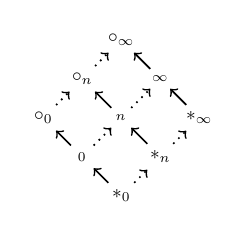
\begin{tikzpicture}
    [->,auto,semithick, every node/.style={scale=0.7}]
    \node(U) {$\kun_0$} ;
    \node(A) [above left of=U] {$\kaff_0$} ;
    \node(L) [above left of=A] {$\klin_0$} ;
    \node(Un) [above right of=U] {$\kun_n$} ;
    \node(An) [above left of=Un] {$\kaff_n$} ;
    \node(Ln) [above left of=An] {$\klin_n$} ;
    \node(Uinf) [above right of=Un] {$\kun_\infty$} ;
    \node(Ainf) [above left of=Uinf] {$\kaff_\infty$} ;
    \node(Linf) [above left of=Ainf] {$\klin_\infty$} ;
    \path
    (U) edge (A)
    (A) edge (L)
    (Un) edge (An)
    (An) edge (Ln)
    (Uinf) edge (Ainf)
    (Ainf) edge (Linf)
    ;
    \path[dotted]
    (U) edge (Un)
    (A) edge (An)
    (L) edge (Ln)
    (Un) edge (Uinf)
    (An) edge (Ainf)
    (Ln) edge (Linf)
    ;
  \end{tikzpicture}
\end{minipage}

%%% Local Variables:
%%% mode: latex
%%% TeX-master: "../main"
%%% End:

  \caption{Lattice inequalities -- $k \lk_\Lat k'$}
  \begin{mathpar}
  \inferrule{l \leq_{\mathcal L} l'}{\entail{}{\Cleq{l}{l'}}}
  \and
  \inferrule{}{\entail{}{\Cleq{k}{\klin_\infty}}}
  \and
  \inferrule{}{\entail{}{\Cleq{\kun_0}{k}}}
  \and
  \inferrule
  {}{ \entail{}{\Cleq{\kvar}{\kvar}} }
  % \and
  % \inferrule
  % {\Cleq{k}{k'} \in C}{ \entail{C}{\Cleq{k}{k'}} }
  % \and
  % \inferrule
  % { \entail{C}{\Cleq{x_1}{x}}\\
  %   \entail{C}{\Cleq{x}{x_2}}
  % }
  % { \entail{C}{\Cleq{x_1}{x_2}} }
  % \and
  % \inferrule
  % { \entail{C}{D} }
  % { \entail{C}{\Cproj{x}{D}} }
  \\
  \inferrule
  { \entail{C}{\Cleq{\tau'_1}{\tau_1}}\\
    \entail{C}{\Cleq{\tau_2}{\tau'_2}}\\
    \entail{C}{\Cleq{k}{k'}}
  }
  { \entail{C}{\Cleq{\tau_1\tarr{k}\tau_2}{\tau'_1\tarr{k'}\tau'_2}} }
  \and
  \inferrule
  { \forall i,\ \entail{C}{\Ceq{\tau_i}{\tau_i}}\\
  }
  { \entail{C}{\Cleq{\tapp{t}{(\tau_i)}}{\tapp{t}{(\tau'_i)}}} }
  % \and
  % \inferrule
  % { \entail{C}{\Cleq{k}{k'}} \\
  %   \entail{C}{\Cleq{k'}{k}} }
  % { \entail{C}{\Ceq{k}{k'}} }
  % \and
  % \inferrule
  % { \entail{C}{\Cleq{k}{k'}} }
  % { \entail{C}{\Ckind{\tau_0\tarr{k}\tau_1}}{k'}}
  % \and
  % \text{Completion to form a cylindric constraint system.}
\end{mathpar}

%%% Local Variables:
%%% mode: latex
%%% TeX-master: "../main"
%%% End:

  \caption{Base entailment rules -- $\entail{C}{D}$ }
  \label{rules:entail}
\end{figure}


We note $\SC$ the set of solved forms
which can be used inside type and kind schemes.
We define $\SC$ as $\A$ quotiented by the relation $\equivC$.
%
We consider the existence of a function $\operatorname{normalize}$ which takes
a constraint in $\A$ and a substitution $\psi$ and returns a constraint
in solved form $C' \in \SC$,
and an updated substitution. We detail the implementation
of the normalization function in \cref{infer:solving}

% $\mathcal S$ is composed only of kind
% inequalities \emph{over variables}. For convenience, if $C\in\mathcal S$, we
% note $C$ as a list of kind inequalities: $\Cleq{\kvar_i}{\kvar_{i'}}^n$.
% \TODO{Extend the properties of solved forms}

\subsection{Kinding}

We note $\inferSK{C}{\E}{\tau}{k}$
when $\tau$ has kind $k$ in environment $\E$ under constraints $C$.
The rules are shown in \cref{rules:sd-kinding}.
Kinds and types follow a small calculus with variables ($\tvar$,\dots),
functions (type constructors $\T{t}$), application ($\tapp{t}{\Multi{\tau}}$)
and primitives such as types for arrows ($\tau\tarr{k}\tau'$) and
borrows ($\borrowty{k}{\tau}$).
Kind checking can thus be done in a fairly straightforward, syntax-directed
fashion by simply following
the syntax of the types. Kind arrows can only appear when looking
up the kind scheme of a type constructor $\T t$. Kind arrows are forbidden
in any other contexts.


\begin{figure}[ht]
  \centering
  \begin{mathpar}
  \inferrule[KVar]
  { \bvar{\tvar}{k} \in \E }
  { \inferSK{C}{\E}{\tvar}{k}
  }
  \and
  \inferrule[KArr]
  {}
  { \inferSK{C}{\E}{\tau_1 \tarr{k} \tau_2}{k} }
  \and
  \inferrule[KApp]
  { \bvar{\T{\tcon}}{
      \forall \Multi[i]\kvar.\ \qual{D}{(\Multi[j]{k'}) \karr k'}}
    \in \E \\
    \inferSK{C}{\E}{\Multi[j]{\tau}}{\Multi[j]{k}} \\
    \unif = \subst{\Multi[i]\kvar}{\Multi[i]k}{} \\
    \entail C {\unif D} \\
    \inferSS{C}{\E}{\Multi[j]k}{\unif{\Multi[j]{k'}}}
  }
  { \inferSK{C}{\E}{\tapp{\tcon}{\Multi[j]{\tau}}}{\unif{k'}} }
  \and
  \inferrule[KBorrow]
  {}{ \inferSK{C}{\E}{\borrowty{k}{\tau}}{k}}
  \and
  \inferrule[KPair]
  { \forall i \quad
    \inferSK{C}{\E}{\tau_i}{k_i} \quad
    \inferSS{C}{\E}{k_i}{k}
  }
  { \inferSK{C}{\E}{\tyPair{\tau_1}{\tau_2}}{k} }
\end{mathpar}


%%% Local Variables:
%%% mode: latex
%%% TeX-master: "../main"
%%% End:

  \caption{Syntax-directed kinding rule --
    $\inferSK{C}{\E}{\tau}{k}$}
  \label{rules:sd-kinding}
\end{figure}

\subsection{Environments}
\label{typ:extra:envs}

\begin{figure}[tp]
  \begin{minipage}{0.38\linewidth}
\begin{mathpar}
  \inferrule[ESplit-Empty]{}{
    \bsplit{\Cempty}\Eempty\Eempty\Eempty
  }

  \inferrule[ESplit-Nonempty]{
    \bsplit{C_1}{\E}{\E_1}{\E_2} \\
    \bsplit{C_2}{b}{b_1}{b_2}
  }{
    \bsplit{C_1\Cand C_2}{\E;b}{\E_1;b_1}{\E_2;b_2}
  }

  \inferrule[ESplit-Check]{
    \bsplit{D}{\E}{\E_1}{\E_2} \\
    \entail{C}{D}
  }{
    \lsplit{C}{\E}{\E_1}{\E_2}
  }
\end{mathpar}
\end{minipage}\vrule~
\begin{minipage}{0.6\linewidth}
    \begin{tabular}
      {@{}>{$}r<{$}@{ $\Lleftarrow$ }
      >{$}c<{$}@{ $=$ }
      >{$}c<{$}@{ $\ltimes$ }
      >{$}c<{$}r}
      
      \Cleq{\schm}{\kun_\infty}
      &\bvar{x}{\schm}&\bvar{x}{\schm}&\bvar{x}{\schm}
      &Both\\[2mm]

      {\Cempty}&
      {\bvar{\borrow[\IBORROW]{x}}{\schm}}&
      {\bvar{\borrow[\IBORROW]{x}}{\schm}}&{\bvar{\borrow[\IBORROW]{x}}{\schm}}
      &Borrow\\[2mm]

      {\Cempty}&{\bvar{x}{\schm}}&{\bvar{x}{\schm}}&{\bnone}
      &Left\\
      {\Cempty}&{\bvar{x}{\schm}}&{\bnone}&{\bvar{x}{\schm}}
      &Right\\[2mm]

      {\Cempty}&{\bvar x \schm}&{\svar x \schm^n}&{\bvar x \schm}
      &Susp\\

      {\Cempty}&
      {\bvar{\borrow x} \schm}&{\svar[\IBORROW] x \schm^n}&{\bvar{\borrow x} \schm}
      &SuspB\\

    \end{tabular}
\end{minipage}

% \begin{mathpar}
%   \inferrule[BSplit-Both]{}{
%     \bsplit {\Cleq{\schm}{\kun_\infty}}
%     {\bvar{x}{\schm}} {\bvar{x}{\schm}} {\bvar{x}{\schm}}
%   }

%   \inferrule[BSplit-Left]{}{
%     \bsplit {\Cempty} {\bvar{x}{\schm}} {\bvar{x}{\schm}} {\bnone}
%   }

%   \inferrule[BSplit-Right]{}{
%     \bsplit {\Cempty} {\bvar{x}{\schm}} {\bnone} {\bvar{x}{\schm}}
%   }

%   \inferrule[BSplit-Imm-Borrow]{}{
%     \bsplit {\Cempty}
%     {\bvar{\borrow[\IBORROW]{x}}{\schm}}
%     {\bvar{\borrow[\IBORROW]{x}}{\schm}}{\bvar{\borrow[\IBORROW]{x}}{\schm}}
%   }

%   \inferrule[BSplit-To-Borrow]{}{
%     \bsplit {\Cempty}{\bvar x \schm}{\svar x \schm^n}{\bvar x \schm}
%   }

%   \inferrule[BSplit-To-Imm]{}{
%     \bsplit {\Cempty}
%     {\bvar{\borrow x} \schm}{\svar[\IBORROW] x \schm^n}{\bvar{\borrow x} \schm}
%   }
% \end{mathpar}
%%% Local Variables:
%%% mode: latex
%%% TeX-master: "../main"
%%% End:

  \caption{Splitting --- environments $\lsplit
    C\E\E\E$; binders $\bsplit Cbbb$}
  \label{fig:sd-splitting}
\end{figure}

\begin{figure}[tp]
  \begin{mathpar}
  \inferrule[EBorrow]{
    \bregion{C_r}{}{\svar{x}{\tau}^n}{b}
  }{
    \bregion{C_r}{x}{\E;\svar{x}{\tau}^n}{\E; b}
  }

  \inferrule[EBorrow-Check]{
    \bregion{D}{x}{\E;\svar{x}{\tau}^n}{\E; b} \\
    \entail{C}{D}
  }{
    \lregion{C}{x}{\E;\svar{x}{\tau}^n}{\E; b}
  }
\end{mathpar}
\hrulefill
\begin{mathpar}
  \inferrule[BSplit-Immut]{}{
    \bregion{(\kun_n\lk k\lk\kun_\infty)}{}
    {\svar[\IBORROW]{x}{\tau}^n}{\bvar{\borrow[\IBORROW]{x}}{\borrowty[\IBORROW] k{\tau}}}
  }
  \and
  \inferrule[BSplit-Mut]{}{
    \bregion{(\kaff_n\lk k\lk\kaff_\infty)}{}
    {\svar[\MBORROW]{x}{\tau}^n}{\bvar{\borrow[\MBORROW]{x}}{\borrowty[\MBORROW] k{\tau}}}
  }
\end{mathpar}
%%% Local Variables:
%%% mode: latex
%%% TeX-master: "../main"
%%% End:

  \caption{Borrowing --- environments $\lsplit
    C\E\E\E$; binders $\bsplit Cbbb$}
  \label{fig:sd-borrowing}
\end{figure}

\subsection{Typing}

\begin{figure*}[tp]
  \begin{mathpar}
  \inferrule{}{ \Cleq{\Eempty}{k} = \Cempty}

  \inferrule{
    \Cleq\E k = C_1 \\ \Cleq B k = C_2
  }{
    \Cleq{\E; B}{k} = C_1 \Cand C_2
  }

  \inferrule{
    \Cleq \tau k = C
  }{ \Cleq{\bvar x \tau}{k} = C}

  \inferrule{
    \Cleq \tau k = C_1 \\
    \BORROW ??? C_2
  }{
    \Cleq{\svar x \tau} k = C_1 \Cand C_2
  }

  \inferrule{}
  { \Cleq{ \tau_2\tarr{k'}\tau_1 } k = \Cleq{k'}k }

  \inferrule{
    \tvar : \kschm
  }
  { \Cleq{ \tvar} k = \Cleq\kschm k }

  \inferrule{
  }{ \Cleq{\tapp{t}{\Multi\tau}} k = ???}

  \inferrule{}{
    \Cleq{\borrow{\tau}} k = ???
  }
\end{mathpar}

%%% Local Variables:
%%% mode: latex
%%% TeX-master: "../main"
%%% End:

  \caption{Rewriting constraints on environments and types}
  \label{fig:contraints-environments-types}
\end{figure*}
\begin{figure*}[tp]
  % \begin{mathpar}
%   \inferrule[Scheme]{
%     \inferSK{C \Cand C_x} \E \tau {k'} \\
%     \entail C {\Cleq{k'}k}
%   }{
%     \entail C {(\forall \kvar_i \forall (\tvar_j:k_j).\
%       \qual{C_x}{\tau}) \le  k}
%   }
% \end{mathpar}
% \hrulefill
\begin{mathpar}
  \ruleSDConst
  \and
  \ruleSDVar
  \and
  \ruleSDLam
  \and
  \ruleSDBorrow
  \and
  \ruleSDReBorrow
  \and
  \ruleSDPair
  \and
  \ruleSDRegion
  \and
  \ruleSDApp
  \and
  \ruleSDLet
  \and
  \ruleSDMatchPair
  \and
  \ruleSDCreate
  \and
  \ruleSDObserve
  \and
  \ruleSDUpdate
  \and
  \ruleSDDestroy
  % \and
  %
  %
  % \inferrule[Elim]
  % { \tvar,(\kvar'_i),(\tvar'_j)\text{ new}\\
  %   \bvar{K}{
  %     \forall \kvar_i \forall (\tvar_j:\kvar_j).\ \qual{C_K}{\tau_1 \tarr{}\tau_2}
  %   } \in \E\\
  %   \inferW{\Sv}{(C,\unif)}{\E}{e}{\tau} \\
  %   \unif' =
  %   \subst{\kvar_i}{\kvar'_i}{} \meet
  %   \subst{\tvar_j}{\tvar'_j}{} \meet \unif \\
  %   D =
  %   C \Cand C_K \Cand \Cleq{\tau_1}{\tvar} \Cand \Cleq{\tau}{\tau_2} \\
  %   (C,\unif) = \normalize{D}{\unif'}\\
  % }
  % { \inferW{\addlin{\Sv}}{(C,\unif|_{\fv{\E}})}{\E}{\elimK{K}{e}}
  %   {\unif\tvar} }
\end{mathpar}

% \begin{align*}
%   \Weaken(x,\Sv)
%   &\equiv \begin{cases}
%     \operatorname{kind}(x)\lk\kun &\text{if } \operatorname{kind}(x)\in\Sv\\
%     \Cempty &\text{otherwise}
%   \end{cases}\\
%   \Cleq{\Sv}{k}
%   &\equiv \bigwedge_{\kvar\in\Sv} \Cleq{\kvar}{k}
% \end{align*}

%%% Local Variables:
%%% mode: latex
%%% TeX-master: "../main"
%%% End:

  \caption{Syntax-directed typing rules}
  \label{fig:syntax-directed-typing}
\end{figure*}

%%% Local Variables:
%%% mode: latex
%%% TeX-master: "../main"
%%% End:

\clearpage
\section{Annotating regions}
\label{regionannot}

So far, all \lang programs have been fully annotated with regions information.
We now show how to infer these regions annotations based on
optionally-annotated programs.
First, we extend the region annotation to $\region{S}{E}$ where $S$ is
a set of variables. This annotation, defined below, is equivalent to nested
region annotations for each individual variable.

\begin{align*}
  \region{x;S}{e} &= \region{x}{\region{S}{e}}& \region{\emptyset}{e} &= e\\
\end{align*}

\Cref{fig:region-annotation} define a rewriting relation $\RannotT{e}{e'}$
which indicates that an optionally annotated term $e$ can be written
in a fully annotated term $e'$.
Through the rule \textsc{Rewrite-Top}, this is defined
in term of an inductively defined relation
$\Rannot{e}{e'}{S}$ where $n$ is the current nesting and $S$ is a set of
variable that are not enclosed in a region yet.
The base cases are constants, variables and borrows.
The general idea is to start from the leafs of the syntax tree, create a
region for each borrow, and enlarge the region as much as possible.
This is implemented by a depth-first walk of the syntax
tree which collects each variable that has a corresponding borrow.
At each step, it rewrites the inner subterms,
consider which borrow must be enclosed by a region now, and
return the others for later enclosing. Binders force immediate
enclosing of the bound variables, as demonstrated in rule \textsc{Rewrite-Lam}.
For nodes with multiple children, we
use a scope merge operator to decide if regions should be placed and where.
This is shown in rule \textsc{Rewrite-Pair}.
The merge operator, written $\getBorrows{B_l}{B_r}{(S_l,S,S_r)}$, takes
the sets $B_l$ and $B_r$ returned by rewriting the subterms
and returns three sets: $S_l$ and $S_r$ indicates the variables
that should be immediately enclosed by a region on the left and right
subterms and $S$ indicates the set of the yet-to-be-enclosed variables.
As an example, the rule \textsc{AnnotRegion-MutLeft} is applied
when there is an immutable borrow and a mutable borrow. In that case, a
region is created to enclose the immutable borrow, while the mutable
borrow is left to be closed later. This is coherent with the rules
for environment splitting and suspended bindings from \cref{sdtyping}.
%
Explicitly annotated regions are handled specially through
rule \textsc{Rewrite-Region}. In that case, we assume that all inner
borrows should be enclosed immediately.

\begin{figure*}[!hbt]
  \centering
  \begin{mathpar}
  \inferrule[AnnotRegion-Empty]{}{
    \getBorrows{\Sempty}{\Sempty}{\Sempty,\Sempty,\Sempty}
  }

  \inferrule[AnnotRegion-Nonempty]{
    \getBorrows{B_1}{B_2}{S_1,S,S_2}\\
    \getBorrows{b_1}{b_2}{S'_1,S',S'_2}
  }{
    \getBorrows{B_1;b_1}{B_2;b_2}
    {S_1\Sunion S'_1,S\Sunion S',S_2\Sunion S'_2}
  }
\end{mathpar}
\hrulefill
\begin{mathpar}
  \inferrule[AnnotRegion-Left]{}{
    \getBorrows
    {\Sone{x}{b}}
    {\Cempty}
    {\Cempty,\Sone{x}{b},\Cempty}
  }
  
  \inferrule[AnnotRegion-Right]{}{
    \getBorrows
    {\Cempty}
    {\Sone{x}{b}}
    {\Cempty,\Sone{x}{b},\Cempty}
  }
  
  \inferrule[AnnotRegion-Immut]{}{
    \getBorrows
    {\Sone{x}{\IBORROW}}
    {\Sone{x}{\IBORROW}}
    {\Cempty,\Sone{x}{\IBORROW},\Cempty}
  }
  
  \inferrule[AnnotRegion-MutLeft]{}{
    \getBorrows
    {\Sone{x}{\IBORROW}}
    {\Sone{x}{\IBORROW}}
    {\Sone{x}{\IBORROW},\Sone{x}{\MBORROW},\Cempty}
  }
  
  \inferrule[AnnotRegion-MutRight]{}{
    \getBorrows
    {\Sone{x}{\MBORROW}}
    {\Sone{x}{\IBORROW}}
    {\Cempty,\Sone{x}{\MBORROW},\Sone{x}{\IBORROW}}
  }
  
  \inferrule[AnnotRegion-Mut]{}{
    \getBorrows
    {\Sone{x}{\MBORROW}}
    {\Sone{x}{\MBORROW}}
    {\Sone{x}{\MBORROW},\Cempty,\Sone{x}{\IBORROW}}
  }
\end{mathpar}
\hrulefill
\begin{mathpar}
  \inferrule{}
  { \Rannot{\borrow{x}}{\borrow{x}}{\Sone{x}{b}} }

  \inferrule
  { \forall i,\ \Rannot{e_i}{e'_i}{B_i} \\
    \getBorrows{B_1}{(B_2\Sdel{x})}{S_1,S,S_2} \\
    S'_2 = S_2\Sunion B_2\Sonly{x}
  }
  { \Rannot
    {\letin{x}{e_1}{e_2}}
    {\letin{x}{\region{S_1}{e'_1}}{\region{S'_2}{e'_2}}}{S} }
  
  \inferrule{e = c\ |\ x}
  { \Rannot{e}{e}{\Sempty} }

  \inferrule
  { \forall i,\ \Rannot{e_i}{e'_i}{B_i} \\
    \getBorrows{B_1}{B_2}{S_1,S,S_2}
  }
  { \Rannot{\app{e_1}{e_2}}{\app{\region{S_1}{e'_1}}{\region{S_2}{e'_2}}}{S} }

  \inferrule
  { \Rannot{e}{e'}{B} \\
    B_x = B\Sonly{x}
  }
  { \Rannot{\lam{x}{e}}{\lam{x}{\region{B_x}{e'}}}{B\Sdel{x}} }

  \inferrule
  { \Rannot{e}{e'}{B} }
  { \Rannot{\regionS{e}}{\region{B}{e'}}{\Sempty} }

  \inferrule
  { \forall i,\ \Rannot{e_i}{e'_i}{B_i} \\
    \getBorrows{B_1}{B_2}{S_1,S,S_2}
  }
  { \Rannot
    {\introPair{e_1}{e_2}}
    {\introPair{\region{S_1}{e'_1}}{\region{S_2}{e'_2}}}
    {S} }

  \inferrule
  { \forall i,\ \Rannot{e_i}{e'_i}{B_i} \\
    \getBorrows{B_1}{(B_2\Sdel{x,y})}{S_1,S,S_2} \\
    S'_2 = S_2\Sunion B_2\Sonly{x,y}
  }
  { \Rannot
    {\matchin{x,y}{e_1}{e_2}}
    {\matchin{x,y}{\region{S_1}{e'_1}}{\region{S'_2}{e'_2}}}{S} }
\end{mathpar}

%%% Local Variables:
%%% mode: latex
%%% TeX-master: "main"
%%% End:

  \caption{Automatic region annotation --- $\RannotT{e}{e'}$}
  \label{fig:region-annotation}
\end{figure*}

\section{Syntax directed typing}
\label{appendix:sdtyping}

\subsection{Constraint language}

\newcommand\A{\mathcal A}
\newcommand\SC{\mathcal S}

Let us note $\A$ our constraint system. The full grammar of constraints is
given in \cref{grammar:constraint}.
$\A$ is defined as the smallest cylindric term constraint system that
satisfies the axiom shown in \cref{rules:entail}.
We follows the traditional HM(X) formulation
with conjunctions, projections and type inequalities.
The new element specific to our approach are kind inequalities.
Entailment is noted $\entail{C}{D}$, where $D$ is a consequence of the
constraints $C$.
We say that $C$ and $D$ are equivalent, noted $C \equivC D$,
when $\entail{C}{D}$ and $\entail{D}{C}$.
\TODO{Give the cylindric properties ?}

\begin{figure}[btp]
  \centering
  \begin{align*}
    C &::= \Cleq{\tau_1}{\tau_2}
        \mid \Cleq{k_1}{k_2}
        \mid C_1 \Cand C_2
        \mid \Cproj{\tvar}{C}
        \mid \Cproj{\kvar}{C}
  \end{align*}
  \caption{The constraint language}
  \label{grammar:constraint}
  \begin{minipage}{0.65\linewidth}
  \begin{mathpar}
    \inferrule[Lat-UA]{}{\kun_n \lk_\Lat \kaff_n}
    \and
    \inferrule[Lat-AL]{}{\kaff_n \lk_\Lat \klin_n}
    \and
    \inferrule[Lat-U-Level]{n \lk n'}{\kun_n \lk_\Lat \kun_{n'}}
    \and 
    \inferrule[Lat-A-Level]{n \lk n'}{\kaff_n \lk_\Lat \kaff_{n'}}
    \and 
    \inferrule[Lat-L-Level]{n \lk n'}{\klin_n \lk_\Lat \klin_{n'}}
  \end{mathpar}
\end{minipage}~
\begin{minipage}{0.2\linewidth}
  \centering
  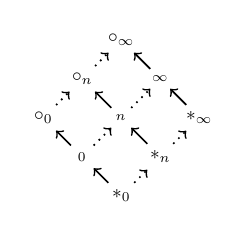
\begin{tikzpicture}
    [->,auto,semithick, every node/.style={scale=0.7}]
    \node(U) {$\kun_0$} ;
    \node(A) [above left of=U] {$\kaff_0$} ;
    \node(L) [above left of=A] {$\klin_0$} ;
    \node(Un) [above right of=U] {$\kun_n$} ;
    \node(An) [above left of=Un] {$\kaff_n$} ;
    \node(Ln) [above left of=An] {$\klin_n$} ;
    \node(Uinf) [above right of=Un] {$\kun_\infty$} ;
    \node(Ainf) [above left of=Uinf] {$\kaff_\infty$} ;
    \node(Linf) [above left of=Ainf] {$\klin_\infty$} ;
    \path
    (U) edge (A)
    (A) edge (L)
    (Un) edge (An)
    (An) edge (Ln)
    (Uinf) edge (Ainf)
    (Ainf) edge (Linf)
    ;
    \path[dotted]
    (U) edge (Un)
    (A) edge (An)
    (L) edge (Ln)
    (Un) edge (Uinf)
    (An) edge (Ainf)
    (Ln) edge (Linf)
    ;
  \end{tikzpicture}
\end{minipage}

%%% Local Variables:
%%% mode: latex
%%% TeX-master: "../main"
%%% End:

  \caption{Lattice inequalities -- $k \lk_\Lat k'$}
  \begin{mathpar}
  \inferrule{l \leq_{\mathcal L} l'}{\entail{}{\Cleq{l}{l'}}}
  \and
  \inferrule{}{\entail{}{\Cleq{k}{\klin_\infty}}}
  \and
  \inferrule{}{\entail{}{\Cleq{\kun_0}{k}}}
  \and
  \inferrule
  {}{ \entail{}{\Cleq{\kvar}{\kvar}} }
  % \and
  % \inferrule
  % {\Cleq{k}{k'} \in C}{ \entail{C}{\Cleq{k}{k'}} }
  % \and
  % \inferrule
  % { \entail{C}{\Cleq{x_1}{x}}\\
  %   \entail{C}{\Cleq{x}{x_2}}
  % }
  % { \entail{C}{\Cleq{x_1}{x_2}} }
  % \and
  % \inferrule
  % { \entail{C}{D} }
  % { \entail{C}{\Cproj{x}{D}} }
  \\
  \inferrule
  { \entail{C}{\Cleq{\tau'_1}{\tau_1}}\\
    \entail{C}{\Cleq{\tau_2}{\tau'_2}}\\
    \entail{C}{\Cleq{k}{k'}}
  }
  { \entail{C}{\Cleq{\tau_1\tarr{k}\tau_2}{\tau'_1\tarr{k'}\tau'_2}} }
  \and
  \inferrule
  { \forall i,\ \entail{C}{\Ceq{\tau_i}{\tau_i}}\\
  }
  { \entail{C}{\Cleq{\tapp{t}{(\tau_i)}}{\tapp{t}{(\tau'_i)}}} }
  % \and
  % \inferrule
  % { \entail{C}{\Cleq{k}{k'}} \\
  %   \entail{C}{\Cleq{k'}{k}} }
  % { \entail{C}{\Ceq{k}{k'}} }
  % \and
  % \inferrule
  % { \entail{C}{\Cleq{k}{k'}} }
  % { \entail{C}{\Ckind{\tau_0\tarr{k}\tau_1}}{k'}}
  % \and
  % \text{Completion to form a cylindric constraint system.}
\end{mathpar}

%%% Local Variables:
%%% mode: latex
%%% TeX-master: "../main"
%%% End:

  \caption{Base entailment rules -- $\entail{C}{D}$ }
  \label{rules:entail}
\end{figure}


We note $\SC$ the set of solved forms
which can be used inside type and kind schemes.
We define $\SC$ as $\A$ quotiented by the relation $\equivC$.
%
We consider the existence of a function $\operatorname{normalize}$ which takes
a constraint in $\A$ and a substitution $\psi$ and returns a constraint
in solved form $C' \in \SC$,
and an updated substitution. We detail the implementation
of the normalization function in \cref{infer:solving}

% $\mathcal S$ is composed only of kind
% inequalities \emph{over variables}. For convenience, if $C\in\mathcal S$, we
% note $C$ as a list of kind inequalities: $\Cleq{\kvar_i}{\kvar_{i'}}^n$.
% \TODO{Extend the properties of solved forms}

\subsection{Kinding}

We note $\inferSK{C}{\E}{\tau}{k}$
when $\tau$ has kind $k$ in environment $\E$ under constraints $C$.
The rules are shown in \cref{rules:sd-kinding}.
Kinds and types follow a small calculus with variables ($\tvar$,\dots),
functions (type constructors $\T{t}$), application ($\tapp{t}{\Multi{\tau}}$)
and primitives such as types for arrows ($\tau\tarr{k}\tau'$) and
borrows ($\borrowty{k}{\tau}$).
Kind checking can thus be done in a fairly straightforward, syntax-directed
fashion by simply following
the syntax of the types. Kind arrows can only appear when looking
up the kind scheme of a type constructor $\T t$. Kind arrows are forbidden
in any other contexts.


\begin{figure}[ht]
  \centering
  \begin{mathpar}
  \inferrule[KVar]
  { \bvar{\tvar}{k} \in \E }
  { \inferSK{C}{\E}{\tvar}{k}
  }
  \and
  \inferrule[KArr]
  {}
  { \inferSK{C}{\E}{\tau_1 \tarr{k} \tau_2}{k} }
  \and
  \inferrule[KApp]
  { \bvar{\T{\tcon}}{
      \forall \Multi[i]\kvar.\ \qual{D}{(\Multi[j]{k'}) \karr k'}}
    \in \E \\
    \inferSK{C}{\E}{\Multi[j]{\tau}}{\Multi[j]{k}} \\
    \unif = \subst{\Multi[i]\kvar}{\Multi[i]k}{} \\
    \entail C {\unif D} \\
    \inferSS{C}{\E}{\Multi[j]k}{\unif{\Multi[j]{k'}}}
  }
  { \inferSK{C}{\E}{\tapp{\tcon}{\Multi[j]{\tau}}}{\unif{k'}} }
  \and
  \inferrule[KBorrow]
  {}{ \inferSK{C}{\E}{\borrowty{k}{\tau}}{k}}
  \and
  \inferrule[KPair]
  { \forall i \quad
    \inferSK{C}{\E}{\tau_i}{k_i} \quad
    \inferSS{C}{\E}{k_i}{k}
  }
  { \inferSK{C}{\E}{\tyPair{\tau_1}{\tau_2}}{k} }
\end{mathpar}


%%% Local Variables:
%%% mode: latex
%%% TeX-master: "../main"
%%% End:

  \caption{Syntax-directed kinding rule --
    $\inferSK{C}{\E}{\tau}{k}$}
  \label{rules:sd-kinding}
\end{figure}

\subsection{Environments}
\label{typ:extra:envs}

\begin{figure}[tp]
  \begin{minipage}{0.38\linewidth}
\begin{mathpar}
  \inferrule[ESplit-Empty]{}{
    \bsplit{\Cempty}\Eempty\Eempty\Eempty
  }

  \inferrule[ESplit-Nonempty]{
    \bsplit{C_1}{\E}{\E_1}{\E_2} \\
    \bsplit{C_2}{b}{b_1}{b_2}
  }{
    \bsplit{C_1\Cand C_2}{\E;b}{\E_1;b_1}{\E_2;b_2}
  }

  \inferrule[ESplit-Check]{
    \bsplit{D}{\E}{\E_1}{\E_2} \\
    \entail{C}{D}
  }{
    \lsplit{C}{\E}{\E_1}{\E_2}
  }
\end{mathpar}
\end{minipage}\vrule~
\begin{minipage}{0.6\linewidth}
    \begin{tabular}
      {@{}>{$}r<{$}@{ $\Lleftarrow$ }
      >{$}c<{$}@{ $=$ }
      >{$}c<{$}@{ $\ltimes$ }
      >{$}c<{$}r}
      
      \Cleq{\schm}{\kun_\infty}
      &\bvar{x}{\schm}&\bvar{x}{\schm}&\bvar{x}{\schm}
      &Both\\[2mm]

      {\Cempty}&
      {\bvar{\borrow[\IBORROW]{x}}{\schm}}&
      {\bvar{\borrow[\IBORROW]{x}}{\schm}}&{\bvar{\borrow[\IBORROW]{x}}{\schm}}
      &Borrow\\[2mm]

      {\Cempty}&{\bvar{x}{\schm}}&{\bvar{x}{\schm}}&{\bnone}
      &Left\\
      {\Cempty}&{\bvar{x}{\schm}}&{\bnone}&{\bvar{x}{\schm}}
      &Right\\[2mm]

      {\Cempty}&{\bvar x \schm}&{\svar x \schm^n}&{\bvar x \schm}
      &Susp\\

      {\Cempty}&
      {\bvar{\borrow x} \schm}&{\svar[\IBORROW] x \schm^n}&{\bvar{\borrow x} \schm}
      &SuspB\\

    \end{tabular}
\end{minipage}

% \begin{mathpar}
%   \inferrule[BSplit-Both]{}{
%     \bsplit {\Cleq{\schm}{\kun_\infty}}
%     {\bvar{x}{\schm}} {\bvar{x}{\schm}} {\bvar{x}{\schm}}
%   }

%   \inferrule[BSplit-Left]{}{
%     \bsplit {\Cempty} {\bvar{x}{\schm}} {\bvar{x}{\schm}} {\bnone}
%   }

%   \inferrule[BSplit-Right]{}{
%     \bsplit {\Cempty} {\bvar{x}{\schm}} {\bnone} {\bvar{x}{\schm}}
%   }

%   \inferrule[BSplit-Imm-Borrow]{}{
%     \bsplit {\Cempty}
%     {\bvar{\borrow[\IBORROW]{x}}{\schm}}
%     {\bvar{\borrow[\IBORROW]{x}}{\schm}}{\bvar{\borrow[\IBORROW]{x}}{\schm}}
%   }

%   \inferrule[BSplit-To-Borrow]{}{
%     \bsplit {\Cempty}{\bvar x \schm}{\svar x \schm^n}{\bvar x \schm}
%   }

%   \inferrule[BSplit-To-Imm]{}{
%     \bsplit {\Cempty}
%     {\bvar{\borrow x} \schm}{\svar[\IBORROW] x \schm^n}{\bvar{\borrow x} \schm}
%   }
% \end{mathpar}
%%% Local Variables:
%%% mode: latex
%%% TeX-master: "../main"
%%% End:

  \caption{Splitting --- environments $\lsplit
    C\E\E\E$; binders $\bsplit Cbbb$}
  \label{fig:sd-splitting}
\end{figure}

\begin{figure}[tp]
  \begin{mathpar}
  \inferrule[EBorrow]{
    \bregion{C_r}{}{\svar{x}{\tau}^n}{b}
  }{
    \bregion{C_r}{x}{\E;\svar{x}{\tau}^n}{\E; b}
  }

  \inferrule[EBorrow-Check]{
    \bregion{D}{x}{\E;\svar{x}{\tau}^n}{\E; b} \\
    \entail{C}{D}
  }{
    \lregion{C}{x}{\E;\svar{x}{\tau}^n}{\E; b}
  }
\end{mathpar}
\hrulefill
\begin{mathpar}
  \inferrule[BSplit-Immut]{}{
    \bregion{(\kun_n\lk k\lk\kun_\infty)}{}
    {\svar[\IBORROW]{x}{\tau}^n}{\bvar{\borrow[\IBORROW]{x}}{\borrowty[\IBORROW] k{\tau}}}
  }
  \and
  \inferrule[BSplit-Mut]{}{
    \bregion{(\kaff_n\lk k\lk\kaff_\infty)}{}
    {\svar[\MBORROW]{x}{\tau}^n}{\bvar{\borrow[\MBORROW]{x}}{\borrowty[\MBORROW] k{\tau}}}
  }
\end{mathpar}
%%% Local Variables:
%%% mode: latex
%%% TeX-master: "../main"
%%% End:

  \caption{Borrowing --- environments $\lsplit
    C\E\E\E$; binders $\bsplit Cbbb$}
  \label{fig:sd-borrowing}
\end{figure}

\subsection{Typing}

\begin{figure*}[tp]
  \begin{mathpar}
  \inferrule{}{ \Cleq{\Eempty}{k} = \Cempty}

  \inferrule{
    \Cleq\E k = C_1 \\ \Cleq B k = C_2
  }{
    \Cleq{\E; B}{k} = C_1 \Cand C_2
  }

  \inferrule{
    \Cleq \tau k = C
  }{ \Cleq{\bvar x \tau}{k} = C}

  \inferrule{
    \Cleq \tau k = C_1 \\
    \BORROW ??? C_2
  }{
    \Cleq{\svar x \tau} k = C_1 \Cand C_2
  }

  \inferrule{}
  { \Cleq{ \tau_2\tarr{k'}\tau_1 } k = \Cleq{k'}k }

  \inferrule{
    \tvar : \kschm
  }
  { \Cleq{ \tvar} k = \Cleq\kschm k }

  \inferrule{
  }{ \Cleq{\tapp{t}{\Multi\tau}} k = ???}

  \inferrule{}{
    \Cleq{\borrow{\tau}} k = ???
  }
\end{mathpar}

%%% Local Variables:
%%% mode: latex
%%% TeX-master: "../main"
%%% End:

  \caption{Rewriting constraints on environments and types}
  \label{fig:contraints-environments-types}
\end{figure*}
\begin{figure*}[tp]
  % \begin{mathpar}
%   \inferrule[Scheme]{
%     \inferSK{C \Cand C_x} \E \tau {k'} \\
%     \entail C {\Cleq{k'}k}
%   }{
%     \entail C {(\forall \kvar_i \forall (\tvar_j:k_j).\
%       \qual{C_x}{\tau}) \le  k}
%   }
% \end{mathpar}
% \hrulefill
\begin{mathpar}
  \ruleSDConst
  \and
  \ruleSDVar
  \and
  \ruleSDLam
  \and
  \ruleSDBorrow
  \and
  \ruleSDReBorrow
  \and
  \ruleSDPair
  \and
  \ruleSDRegion
  \and
  \ruleSDApp
  \and
  \ruleSDLet
  \and
  \ruleSDMatchPair
  \and
  \ruleSDCreate
  \and
  \ruleSDObserve
  \and
  \ruleSDUpdate
  \and
  \ruleSDDestroy
  % \and
  %
  %
  % \inferrule[Elim]
  % { \tvar,(\kvar'_i),(\tvar'_j)\text{ new}\\
  %   \bvar{K}{
  %     \forall \kvar_i \forall (\tvar_j:\kvar_j).\ \qual{C_K}{\tau_1 \tarr{}\tau_2}
  %   } \in \E\\
  %   \inferW{\Sv}{(C,\unif)}{\E}{e}{\tau} \\
  %   \unif' =
  %   \subst{\kvar_i}{\kvar'_i}{} \meet
  %   \subst{\tvar_j}{\tvar'_j}{} \meet \unif \\
  %   D =
  %   C \Cand C_K \Cand \Cleq{\tau_1}{\tvar} \Cand \Cleq{\tau}{\tau_2} \\
  %   (C,\unif) = \normalize{D}{\unif'}\\
  % }
  % { \inferW{\addlin{\Sv}}{(C,\unif|_{\fv{\E}})}{\E}{\elimK{K}{e}}
  %   {\unif\tvar} }
\end{mathpar}

% \begin{align*}
%   \Weaken(x,\Sv)
%   &\equiv \begin{cases}
%     \operatorname{kind}(x)\lk\kun &\text{if } \operatorname{kind}(x)\in\Sv\\
%     \Cempty &\text{otherwise}
%   \end{cases}\\
%   \Cleq{\Sv}{k}
%   &\equiv \bigwedge_{\kvar\in\Sv} \Cleq{\kvar}{k}
% \end{align*}

%%% Local Variables:
%%% mode: latex
%%% TeX-master: "../main"
%%% End:

  \caption{Syntax-directed typing rules}
  \label{fig:syntax-directed-typing}
\end{figure*}

%%% Local Variables:
%%% mode: latex
%%% TeX-master: "../main"
%%% End:

\clearpage
\section{Semantics definitions}
\label{sec:semant-defin}

% \begin{figure*}[ht]
  % \begin{mathpar}
  \inferrule[Lam]
  { j \fresh }
  { \ered{\closure{j}{x}{e}}{\emptyset}{\lam{x}{e}}{\closure{j}{x}{e}} }
  \and
  \inferrule[App]
  { \ered{I}{E}{f}{\closure{j}{x}{e_f}} \\
    \ered{I'}{E'}{e}{v} \\
    \ered{I''}{E''}{\subst{x}{v}{e_f}}{v_f}
  }
  { \ered{I,I',I''}{E,E',E'',\closure{j}{x}{e_f}}{\app{f}{e}}{v_f} }
  \and
  \inferrule[Let]
  { \ered{I}{E}{e}{v} \\
    \ered{I'}{E'}{\subst{x}{v}{e'}}{v'}
  }
  { \ered{I,I'}{E,E'}{\letin{x}{e}{e'}}{v'} }
\end{mathpar}
%%% Local Variables:
%%% mode: latex
%%% TeX-master: "main"
%%% End:

  \begin{minipage}[t]{0.48\linewidth}
  \begin{align*}
    \htag{Addresses}
    \alpha &::= \ell \tag{Locations}\\
           &\mid \borrow{\alpha} \tag{Borrowed Locations}
    \\
    \htag{Results}
    r &::= \alpha \mid c
  \end{align*}
  \end{minipage}
  \hfill
  \begin{minipage}[t]{0.48\linewidth}
\begin{align*}
    \htag{Storables}
    W &::= (\rho, \closure{k}{x}{e}) \tag{Closures} \\
           &\mid (r, r) \tag{Pairs} \\
    & \mid [r] \tag{Resources}
  \end{align*}
  \end{minipage}
    \begin{mathpar}
    \inferrule{}{ \Sigma, \rho \vdash c \Downarrow \Sigma, c}

    \inferrule{}{\Sigma, \rho \vdash x \Downarrow \Sigma, \rho(x)}

    \inferrule{
      \ell\notin\Dom\Sigma \\
      \Sigma' = \Sigma[\ell \mapsto (\rho, \closure{}{x}{e})]
    }{
      \Sigma, \rho \vdash \lam xe \Downarrow \Sigma', \ell
    }
    
    \inferrule{
      \Sigma, \rho \vdash e \Downarrow \Sigma', \ell \\
      \Sigma' (\ell) = (\rho'',\closure{}{x}{e''}) \\
      \Sigma', \rho \vdash e' \Downarrow \Sigma'', r' \\
      \Sigma'', \rho''[x\mapsto r'] \vdash e'' \Downarrow \Sigma''', r
    }{\Sigma, \rho \vdash \app{e}{e'} \Downarrow \Sigma''', r}

    \inferrule{
      \Sigma, \rho \vdash e \Downarrow \Sigma', r \\
      \Sigma', \rho[x \mapsto r] \vdash e' \Downarrow \Sigma'', r'
    }{
      \Sigma, \rho \vdash \letin{x}{e}{e'} \Downarrow \Sigma'', r'
    }

    \inferrule{
      \Sigma, \rho \vdash e \Downarrow \Sigma', r \\
      \Sigma', \rho \vdash e' \Downarrow \Sigma'', r' \\
      \ell\notin\Dom{\Sigma''} \\
      \Sigma''' = \Sigma''[\ell \mapsto (r, r')]
    }{
      \Sigma, \rho \vdash \introPair{e}{e'} \Downarrow \Sigma''', \ell
    }

    \inferrule{
      \Sigma, \rho \vdash e \Downarrow \Sigma', \ell \\
      \Sigma' (\ell) = (r, r') \\
      \Sigma', \rho[x,y \mapsto r, r'] \vdash e' \Downarrow \Sigma'', r''
    }{
      \Sigma, \rho \vdash \matchin{x,y}{e}{e'} \Downarrow  \Sigma'', r''
    }

    \inferrule{
      \rho (x) = \alpha \\
      \Sigma (\alpha) = W \\
      (\Sigma\setminus\alpha)[\borrow{\alpha} \mapsto W], \rho \vdash e
      \Downarrow \Sigma', r \\
      \Sigma'' = (\Sigma' \setminus\borrow{\alpha})[\alpha \mapsto W]
    }{
      \Sigma, \rho \vdash \region{x}{e} \Downarrow \Sigma', r
    }

    \inferrule{\rho (x) = \alpha}{
      \Sigma, \rho \vdash \borrow{x} \Downarrow \Sigma, \borrow\alpha
    }
    \\
    \inferrule{
      \Sigma, \rho \vdash e \Downarrow \Sigma', r\\
      \ell\notin \Dom\Sigma' }{
      \Sigma,\rho \vdash \create e \Downarrow \Sigma'[\ell \mapsto \rss{r}], \ell
    }

    \inferrule{
      \Sigma, \rho \vdash e \Downarrow \Sigma', \ell \\
      \Sigma' (\ell) = \rss{r}
    }{
      \Sigma, \rho \vdash \destroy e \Downarrow \Sigma'\setminus\ell, ()
    }

    \inferrule{
      \Sigma, \rho \vdash e \Downarrow \Sigma', \borrow[i]\alpha \\
      \Sigma' (\borrow[i]\alpha) = \rss{r}
    }{
      \Sigma, \rho \vdash \observe e \Downarrow \Sigma', r
    }

    \inferrule{
      \Sigma, \rho \vdash e \Downarrow \Sigma', \borrow[m]\alpha \\
      \Sigma', \rho \vdash e' \Downarrow \Sigma'', r' \\
      \Sigma'' (\borrow[m]\alpha) = \rss{r} \\
      \Sigma''' = \Sigma''[\borrow[m]\alpha \mapsto r']
    }{
      \Sigma, \rho \vdash \update e {e'} \Downarrow \Sigma''', ()
    }

  \end{mathpar}
  \caption{Reduction rules -- $\Sigma, \rho, \vdash e \Downarrow
    \Sigma', r$ }
  \label{fig:reduction}
\end{figure*}


%%% Local Variables:
%%% mode: latex
%%% TeX-master: "main"
%%% End:


% Two figures present the operational semantics in traditional style as
% an evaluation judgment $\Store, \Perm, \VEnv \vdash e \Downarrow
% \Store', \Perm', r$.
% \Cref{fig:reduction} contains the lambda calculus reductions  and
% \cref{fig:reduction-resources} shows the resource-related reductions.

\begin{figure}
  \begin{minipage}[t]{0.52\linewidth}
    \lstinputlisting[style=rule,linerange=eval\ header-(**)]
    {syntax/semanticsannotated.ml}
  \lstsemrule{const}
  \medskip
  \lstsemrule{var}
  \medskip
  \lstsemrule{varinst}
  \medskip
  \lstsemrule{polylam}
  \medskip
  \lstsemrule{sapp}
  \medskip
  \lstsemrule{slet}
  \end{minipage}
  \begin{minipage}[t]{0.47\linewidth}
   \lstsemrule{spair}
  \medskip
   \lstsemrule{smatch}
  \medskip
   \lstsemrule{matchborrow}
  \end{minipage}
  \caption{Big-step interpretation}
  \label{fig:full-big-step-interpretation}
\end{figure}

\begin{figure}[tp]
  \begin{minipage}[t]{0.49\linewidth}
  \lstsemrule{sregion}
  \medskip
  \lstsemrule{sborrow}
  \end{minipage}
  \begin{minipage}[t]{0.49\linewidth}
  \lstsemrule{screate}
  \medskip
  \lstsemrule{sdestroy}
  \medskip
  \lstsemrule{sobserve}
  \medskip
  \lstsemrule{supdate}
  \end{minipage}
  \caption{Big-step interpretation (resources)}
  \label{fig:full-big-step-interpretation-resources}
\end{figure}

%%% Local Variables:
%%% mode: latex
%%% TeX-master: "main"
%%% End:


\cref{fig:full-big-step-interpretation} presents  the full big-step
interpretation. \cref{fig:full-big-step-interpretation-resources}
contains the cases for resources.

%%% Local Variables:
%%% mode: latex
%%% TeX-master: "main"
%%% End:

\section{Proofs for Metatheory}
\label{sec:metatheory:proofs}

\begin{itemize}
\item Borrow compatibility
  $\Multi\IBORROW\Multi\MBORROW \Bcompatible \BORROW$,
  \begin{mathpar}
  \inferrule{}{
    \IBORROW\Multi\IBORROW\Multi\MBORROW \Bcompatible \IBORROW
  }

  \inferrule{}{
    \MBORROW\Multi\MBORROW \Bcompatible \MBORROW
  }
  \end{mathpar}
\item Store typing $ \vdash \Store : \SE$,
  \begin{mathpar}
    \inferrule{
      (\forall \Loc \in \Dom\Store)~~
      \SE \vdash \Store (\Loc) : \SE (\Loc)
    }{ \vdash \Store : \SE }
  \end{mathpar}
\item Relating storables to type schemes $\SE \vdash w : \schm$
  \begin{mathpar}
  \inferrule{
    (\exists \E)~ \SE \vdash \VEnv : \E
    \\
    \inferS{C}{\E, (x:\tau_2)}{e}{\tau_1}
    \\
    \Multi\tvar = \fv{\tau_1,\tau_2} \setminus \fv{\E}
  }{
    \SE \vdash (\VEnv, \ilam {\Multi\kvar}{\Multi\tvar}Ckx{e})
    : \forall\Multi\kvar\forall\Multi{\bvar{\tvar}{k}}.(\qual{C}{\tau_2\tarr{k}\tau_1})
  }
  \end{mathpar}
\item Relating storables to types $ \SE \vdash w : \tau$
  \begin{mathpar}
    \inferrule{
      (\exists \E, C)~ \SE \vdash \VEnv : \E
      \\
      \inferS{C}{\E\bvar x{\tau_2}}{e}{\tau_1}
      \\
      \addlin{\entail{C}{\Cleq{\E}{k}}}
    }{
      \SE \vdash (\VEnv, \lam[k]xe) : \tau_2\tarr{k}\tau_1
    }

    \inferrule{
      \SE \vdash r_1 : \tau_1 \\
      \SE \vdash r_2 : \tau_2
    }{
      \SE \vdash \introPair[k]{r_1}{r_2} : \tyPair[k]{\tau_1}{\tau_2}
    }

    \inferrule{
      \SE \vdash r : \IType{\tcon}{\Multi\tau}
    }{
      \SE \vdash {[r]} : \tapp{\tcon}{\Multi\tau}
    }

    \inferrule{}{
      \SE \vdash \StFreed : \tau
    }
  \end{mathpar}
%\item Relating  results to types $ \SE \vdash r : \tau$,
\item Relating results to type schemes $\SE \vdash r : \schm$
  \begin{mathpar}
  \inferrule{}{ \SE \vdash c : \CType{c} }

  \inferrule{}{ \SE \vdash \ell : \SE (\ell) }

  \inferrule{
    \Multi\IBORROW\Multi\MBORROW \Bcompatible \BORROW \\
    \SE \vdash \Loc  : \tau
  }{  \SE \vdash
    \Multi\IBORROW\Multi\MBORROW\Loc : \borrow{\tau}}
  \end{mathpar}
\item Relating environments to contexts. Here we consider an
  environment $\VEnv = (\Active\VEnv, \MutableBorrows\VEnv,
  \ImmutableBorrows\VEnv, \Suspended\VEnv)$ as a quadruple
  consisting of the active entries in $\Active\VEnv$ and the
  entries for exclusive borrows in $\MutableBorrows\VEnv$ and for
  shared borrows in $\ImmutableBorrows\VEnv$, and suspended entries
  in $\Suspended\VEnv$. The
  suspended entries cannot be used directly, but they can be activated
  by borrowing.

  $\SE \vdash \Active\VEnv, \MutableBorrows\VEnv,
  \ImmutableBorrows\VEnv, \Suspended\VEnv : \E$
\end{itemize}
\begin{mathpar}
  \inferrule{}{\SE \vdash \Sempty, \Sempty, \Sempty, \Sempty : \Eempty}

  \inferrule{
    \SE \vdash \Active\VEnv, \MutableBorrows\VEnv,
    \ImmutableBorrows\VEnv, \Suspended\VEnv : \E
    \\ \SE \vdash r : \schm}
  {\SE \vdash \Active\VEnv[ x\mapsto r], \MutableBorrows\VEnv ,
    \ImmutableBorrows\VEnv, \Suspended\VEnv : \E\bvar x\schm }

  \inferrule{\SE \vdash \Active\VEnv, \MutableBorrows\VEnv,
    \ImmutableBorrows\VEnv, \Suspended\VEnv : \E \\
    \SE \vdash r : \schm}
  { \SE \vdash \Active\VEnv, \MutableBorrows\VEnv,
    \ImmutableBorrows\VEnv, \Suspended\VEnv[ x\mapsto r] : \E\svar x\schm^n }

  \inferrule{\SE \vdash \Active\VEnv, \MutableBorrows\VEnv,
    \ImmutableBorrows\VEnv, \Suspended\VEnv : \E \\ \SE \vdash
    \IBORROW\Addr : \schm}
  {\SE \vdash \Active\VEnv, \MutableBorrows\VEnv,
    \ImmutableBorrows\VEnv[ x\mapsto \IBORROW\Addr], \Suspended\VEnv : \E\bvar{\borrow[\IBORROW] x}{\borrowty[\IBORROW] k{ \schm}} }

  \inferrule{\SE \vdash \Active\VEnv, \MutableBorrows\VEnv,
    \ImmutableBorrows\VEnv, \Suspended\VEnv : \E \\ \SE \vdash
    \MBORROW\Addr : \schm}
  {\SE \vdash \Active\VEnv, \MutableBorrows\VEnv[ x\mapsto \MBORROW\Addr],
    \ImmutableBorrows\VEnv, \Suspended\VEnv
    : \E\bvar{\borrow[\MBORROW] x}{\borrowty[\MBORROW] k{ \schm}} }
\end{mathpar}
\paragraph{Extending environments and stores}
\begin{mathpar}
  \inferrule{}{\SE \le \SE}

  \inferrule{\SE \le \SE' \\ \ell \notin \Dom\Store}{\SE \le \SE' (\ell : \schm)}
\\
  \inferrule{}{\Store\le\Store}

  \inferrule{\Store \le \Store' \\ \ell \notin \Dom\Store
  }{\Store \le \Store'[ \ell \mapsto w] }
\end{mathpar}

\begin{lemma}[Store Weakening]\label{lemma:store-weakening}
  $\SE \vdash \VEnv : \E$ and $\SE \le \SE'$ implies $\SE' \vdash
  \VEnv : \E$.
\end{lemma}

We write $\Rawloc\cdot$ for the function that extracts a multiset of
\emph{raw locations} from a result or from the range of the variable
environment. 

\begin{align*}
  \Rawloc{\Multi\IBORROW\Multi\MBORROW\Loc} &= \{\Loc\} \\
  \Rawloc{c} &= \{ \} \\
  \Rawloc\Eempty &= \{\} \\
  \Rawloc{\VEnv( x \mapsto r)} &= \Rawloc\VEnv \cup \Rawloc r
\end{align*}

We write $\Reach\Store\VEnv$ for the multiset of all \emph{addresses}
reachable from $\Rawloc\VEnv$ 
assuming that $\Rawloc\VEnv \subseteq \Dom\Store$\footnote{In
  mixed comparisons between a multiset and a set, we tacitly convert
  a multiset $M$ to its supporting set $\{ x \mid \MultiNumber x M \ne 0\}$.}.
The function $\Reach\Store\cdot$ is defined in
two steps. First a helper function
for results, storables, and environments.

\begin{align*}
  \RS\Store\Eempty &= \Eempty \\
  \RS\Store{\VEnv (x \mapsto r)} &= \RS\Store\VEnv \cup
                                      \RS\Store r \\
  \RS\Store\Addr &= \{ \Addr \}  \\
  \RS\Store c &= \{ \} \\
  \RS\Store{\StPClosure \VEnv {\Multi\kvar} C k x e} &=
                                       \RS\Store\VEnv
  \\
  \RS\Store{\StClosure \VEnv k x e} &=
                                                   \RS\Store\VEnv
  \\
  \RS\Store{\StPair k {r_1} {r_2}} &=
                                                   \RS\Store{r_1}
                                                   \cup \RS\Store{r_2}
  \\
  \RS\Store{\StRes r} &=
                                   \RS\Store r
  \\
  \RS\Store{\StFreed} &= \{ \}
\end{align*}

This multiset is closed transitively by store lookup. We define 
$\Reach\Store\VEnv$ as the smallest multiset $\REACH$ that fulfills
the following inequations. We assume a nonstandard
model of multisets such that an element $\Loc$ may occur infinitely often as in
$\MultiNumber\Loc\REACH = \infty$. 
\begin{align*}
  \REACH &\supseteq \RS\Store\VEnv \\
  \REACH &\supseteq \RS\Store w & \text{if }
                                     \Multi\IBORROW\Multi\MBORROW\Loc
                                     \in \REACH \wedge w = \Store (\Loc)
\end{align*}

We write $\Affine\SE\Loc$ to express that $\Loc$ points to a resource
that requires at least affine treatment. Borrow types do not appear in
store types as the store only knows about the actual resources.

Define  $\Affine\SE\Loc$ if one of the following cases holds:
\begin{itemize}
\item $\SE (\Loc) =
  \forall\Multi\kvar\forall\Multi{\bvar{\tvar}{k}}.(\qual{C}{\tau_2\tarr{k}\tau_1})$
  and $C \wedge (k \lk \kun_\infty)$ is contradictory;
\item $\SE (\Loc) = \tau_2\tarr{k}{\tau_1}$ and $\Cleq{\kaff}{k}$;
\item $\SE (\Loc) = \tyPair[k]{\tau_1}{\tau_2}$ and $\Cleq \kaff
  k$;
\item $\SE (\Loc) = \tapp{\tcon}{\Multi\tau}$.
% \item if $\SE (\Loc) = \borrow[\MBORROW]\tau$, then $\Loc$ is affine
%   \dots (THAT SHOULDN'T REALLY  BE A STORE TYPE)
% \item if $\SE (\Loc) = \borrow[\IBORROW]\tau$, then $\Loc$ is not affine
%   \dots (THAT SHOULDN'T REALLY  BE A STORE TYPE)
\end{itemize}

We write $\Linear\SE\Loc$ to express that $\Loc$ points to a linear
resource.

Define  $\Linear\SE\Loc$ if one of the following cases holds:
\begin{itemize}
\item $\SE (\Loc) =
  \forall\Multi\kvar\forall\Multi{\bvar{\tvar}{k}}.(\qual{C}{\tau_2\tarr{k}\tau_1})$
  and $C \wedge (k \lk \kaff_\infty)$ is contradictory; 
\item $\SE (\Loc) = \tau_2\tarr{k}{\tau_1}$ and $\Cleq{\klin}{k}$;
\item $\SE (\Loc) = \tyPair[k]{\tau_1}{\tau_2}$ and $\Cleq \klin
  k$;
\item $\SE (\Loc) = \tapp{\tcon}{\Multi\tau}$.
\end{itemize}

\clearpage{}
\begin{theorem}
  Suppose that
  \begin{itemize}
  \item $\inferS{C}{\E}{e}{\tau}$
  \item $\SE \vdash \VEnv : \E$
  \item $\vdash \Store : \SE$
  \item $\Rawloc\Perm \subseteq \Dom\Store$
  \item $\Reach\Store{\Active\VEnv, \MutableBorrows\VEnv,
      \ImmutableBorrows\VEnv} \subseteq \Perm$
  \item $\Rawloc{\Active\VEnv}$,
    $\Rawloc{\MutableBorrows\VEnv}$,
    $\Rawloc{\ImmutableBorrows\VEnv}$, and
    $\Rawloc{\Suspended\VEnv}$ are all disjoint
  % \item  $\VEnv'$ with $\Rawloc{\VEnv'}
  %   \subseteq \Dom\Store$ and $\Dom\VEnv \cap \Dom{\VEnv'}=\emptyset$
  \item Incoming Resources: 
    \begin{itemize}
    \item $\forall \Loc\in \Rawloc{\Reach\Store\VEnv}$,  $\Store (\Loc) \ne
      \StFreed$.
      % suspended bindings must not point to freed resources
    \item $\forall \Loc \in \REACH =\Rawloc{\Reach\Store{\Active\VEnv,\MutableBorrows\VEnv}}$,
      if $\Affine\SE\Loc$ then  $\MultiNumber\Loc\REACH= 1$.
    \end{itemize}
  \item  $i\in\Nat$ and $\Store, \Perm, \VEnv \vdash {e}
    \Downarrow^i R$ and $R\ne \TimeOut$.
  \end{itemize}
  Then,
  $\exists$ $\Store'$, $\Perm'$, $r'$, $\SE'$ such that
  \begin{itemize}
  \item
    $R = \Ok{\Store', \Perm', r'}$
  \item $\SE \le \SE'$, $\Store \le \Store'$,
    $\vdash \Store' : \SE'$
  \item $\SE' \vdash r' : \tau$
  \item $\Rawloc{\Perm'} \subseteq \Dom{\Store'}$
  \item $\Reach{\Store'}{r'} \subseteq \Perm'$
  \item Frame: \\
    For all $\Loc \in \Dom{\Store} \setminus
    \Rawloc{\Reach{\Store'}{\VEnv}}$ it must be that
    \begin{itemize}
    \item $\Store' (\Loc) = \Store (\Loc)$ and
    \item  for any $\Addr$ based on $\Loc$,
      $\Addr \in \Perm \Leftrightarrow \Addr\in\Perm'$.
    \end{itemize}
    %% must be \Store because \Perm has no idea of \Perm'
  \item Immutable borrows: \\
    For all $\Addr \in
    \Reach{\Store'}{\ImmutableBorrows\VEnv}$ with
    $\Rawloc\Addr = \{\Loc\}$, it must be that
    $\Loc\in\Dom\Store$,
    $\Store' (\Loc) = \Store (\Loc) \ne \StFreed$
    and $\Addr\in\Perm'$.
  \item Mutable borrows:\\
    For all $\Addr \in  \Reach{\Store'}{\MutableBorrows\VEnv}$
    with $\Rawloc\Addr = \{\Loc\}$, if
    $\Loc\in\Dom\Store$, then 
    $\Store' (\Loc) \ne \StFreed$
    and $\Addr\in{\Perm'}$ implies $\Addr\in
    \Rawloc\Perm$.
    \\\textbf{PJT: this is a really weak statement! anything else that can be said?}
  \item Resources:
    Let $\REACH' =\Reach{\Store'}{\Active\VEnv}$.
    For all $\Loc$ such that $n= \MultiNumber\Loc\REACH >0$ and $n' =
    \MultiNumber\Loc{\REACH'}$,
    \begin{itemize}
    \item if $\Affine{\SE}\Loc$ then $n=1$ and $n'\le 1$,
    \item if $\Linear{\SE}\Loc$ then $n=1$ and $n' = 0$,
    \item if $n'=0$, then $\Loc\notin\Perm'$.
    \end{itemize}
  \item ReadOnly: For all $\Loc \in \Reach
    {\Store'}{\Active\VEnv}$, if $\neg\Writeable{\SE}\Loc$ then
    $\Store' (\ell) = \Store (\ell)$ and $\Loc\in \Perm'$.
  \item No thin air permission: \\
    For all $\Loc\in \Rawloc{\Perm'}$, $\Loc
    \in \Rawloc\Perm \cup  \Dom{\Store'} \setminus \Dom{\Store}$.
  \end{itemize}
\end{theorem}


\begin{theorem}[OLD]
  Suppose that
  \begin{itemize}
  \item $\inferS{C}{\E}{e}{\tau}$
  \item $\SE \vdash \VEnv : \E$
  \item $\vdash \Store : \SE$
  \item $\Rawloc\Perm \subseteq \Dom\Store$
  \item $\Reach\Store{\Active\VEnv, \MutableBorrows\VEnv, \ImmutableBorrows\VEnv} \subseteq \Perm$
  % \item  $\VEnv'$ with $\Rawloc{\VEnv'}
  %   \subseteq \Dom\Store$ and $\Dom\VEnv \cap \Dom{\VEnv'}=\emptyset$
  \item Incoming Resources: Let $\REACH = \Reach\Store\VEnv$.
    \begin{itemize}
    \item
      For all $\Loc$ such that $\MultiNumber\Loc{\Reach{\Store}{\Active\VEnv}} >0$,
      if $\Affine{\SE}\Loc$ then $\MultiNumber\Loc\REACH= 1$
    \item For all $\Loc$ such that $
      \MultiNumber\Loc{\Reach{\Store}{\MutableBorrows\VEnv}} >0$, it
      must be that $\MultiNumber\Loc\REACH=1$.
    \item For all $\Loc$ such that $
      \MultiNumber\Loc{\Reach{\Store}{\Suspended\VEnv}} >0$, it
      must be that $\MultiNumber\Loc\REACH=1$.
    \end{itemize}
  \item  $i\in\Nat$ and $\Store, \Perm, \VEnv \vdash {e}
    \Downarrow^i R$ and $R\ne \TimeOut$.
  \end{itemize}
  Then,
  $\exists$ $\Store'$, $\Perm'$, $r'$, $\SE'$ such that
  \begin{itemize}
  \item
    $R = \Ok{\Store', \Perm', r'}$
  \item $\SE \le \SE'$, $\Store \le \Store'$,
    $\vdash \Store' : \SE'$
  \item $\Rawloc{\Perm'} \subseteq \Dom{\Store'}$
  \item $\SE' \vdash r' : \tau$
  \item $\Reach{\Store'}{r'} \subseteq \Perm'$
  \item Outside: For all $\Loc \in \Dom{\Store} \setminus
    \Reach{\Store'}{\VEnv}$ it must be that
    $\Store' (\Loc) = \Store (\Loc)$
    and $\Loc\in\Perm \Leftrightarrow \Loc\in\Perm'$.
    %% must be \Store because \Perm has no idea of \Perm'
  \item Immutables: For all $\Loc \in
    \Reach{\Store'}{\ImmutableBorrows\VEnv}$ it must be that
    $\Loc\in\Dom\Store$,
    $\Store' (\Loc) = \Store (\Loc)$
    and $\Loc\in\Perm \Leftrightarrow \Loc\in\Perm'$.
  \item Resources:
    Let $\REACH' =\Reach{\Store'}{\Active\VEnv}$.
    For all $\Loc$ such that $n= \MultiNumber\Loc\REACH >0$ and $n' =
    \MultiNumber\Loc{\REACH'}$,
    \begin{itemize}
    \item if $\Affine{\SE}\Loc$ then $n=1$ and $n'\le 1$,
    \item if $\Linear{\SE}\Loc$ then $n=1$ and $n' = 0$,
    \item if $n'=0$, then $\Loc\notin\Perm'$.
    \end{itemize}
  \item ReadOnly: For all $\Loc \in \Reach
    {\Store'}{\Active\VEnv}$, if $\neg\Writeable{\SE}\Loc$ then
    $\Store' (\ell) = \Store (\ell)$ and $\Loc\in \Perm'$.
  \item No thin air permission: For all $\Loc\in \Perm'$, $\Loc
    \in \Perm \cup  \Dom{\Store'} \setminus \Dom{\Store}$.
  \end{itemize}
\end{theorem}

%\clearpage
\lstMakeShortInline[style=rule]@
\begin{proof}
  By induction on the evaluation of
  @eval \Store \Perm \VEnv i e@.

  The base case is trivial as
  @eval \Store \Perm \VEnv 0 e = \TimeOut@.

  Let now $i>0$ and consider the different cases for expressions.

  \textbf{case $e$ of}
  \lstsemrule{sapp}

  By assumption\\ $\ruleSDApp$.

  As \lstinline{sp}  is evidence for the split in the typing rule,
  we find that
  \begin{align}
    \label{eq:1}
    \SE \vdash \VEnv_1 : \E_1 && \SE \vdash \VEnv_2 : \E_2
  \end{align}

  Hence, we can establish the assumptions for the recursive call
  @eval delta pi gamma_1 i' e_1@.
  \begin{itemize}
  \item  $\inferS{C}{\E_1}{e_1}{\tau_2\tarr{k}\tau_1}$ by inversion of typing
  \item $\SE \vdash \VEnv_1 : \E_1$ by \eqref{eq:1}
  \item $\vdash \Store : \SE$ by assumption
  \item $\Rawloc\Perm \subseteq \Dom\Store$ by assumption
  \item $
    \Reach\Store{\Active{\VEnv_1}, \MutableBorrows{\VEnv_1},
      \ImmutableBorrows{\VEnv_1}}
    \subseteq
    \Reach\Store{\Active\VEnv, \MutableBorrows\VEnv, \ImmutableBorrows\VEnv}
    \subseteq \Perm$
  \item Incoming Resources: For $\REACH_1 = \Reach\Store{\VEnv_1}$.
    \begin{itemize}
    \item
      For all $\Loc$ such that $\MultiNumber\Loc{\Reach{\Store}{\Active{\VEnv_1}}} >0$,
      if $\Affine{\SE}\Loc$ then $\MultiNumber\Loc{\REACH_1}= 1$
    \item For all $\Loc$ such that $
      \MultiNumber\Loc{\Reach{\Store}{\MutableBorrows{\VEnv_1}}} >0$, it
      must be that $\MultiNumber\Loc{\REACH_1}=1$.
    \end{itemize}
  \item $i'<i$ and   @eval \Store \Perm gamma_1 i' e_1@ terminates
    with $R_1 \ne \TimeOut$.
  \end{itemize}
  Hence, we can apply the inductive hypothesis and obtain:
  \begin{gather}
    \label{eq:2}
    R_1 = \Ok{\Store_1, \Perm_1, r_1}
    \\
    \SE \le \SE_1 \qquad
    \Store \le \Store_1 \qquad
    \vdash \Store_1 :    \SE_1
    \\
    \Rawloc{\Perm_1} \subseteq \Dom{\Store_1}
    \\\label{eq:3}
    \SE_1 \vdash r_1 : \tau_2\tarr{k}\tau_1
    \\\label{eq:10}
    \Reach{\Store_1}{r_1} \subseteq \Perm_1
  \end{gather}
  \begin{itemize}
  \item Outside: For all $\Loc \in \Dom{\Store} \setminus
    \Reach{\Store_1}{\VEnv_1}$ it must be that
    $\Store_1 (\Loc) = \Store (\Loc)$
    and $\Loc\in\Perm \Leftrightarrow \Loc\in\Perm_1$
  \item Immutables: For all $\Loc \in
    \Reach{\Store_1}{\ImmutableBorrows{\VEnv_1}}$ it must be that
    $\Loc\in\Dom\Store$,
    $\Store_1 (\Loc) = \Store (\Loc)$
    and $\Loc\in\Perm \Leftrightarrow \Loc\in\Perm_1$
  \item Resources:
    Let $\REACH_1 =\Reach{\Store_1}{\Active{\VEnv_1}}$.
    For all $\Loc$ such that $n= \MultiNumber\Loc{\REACH_1} >0$,
    \begin{itemize}
    \item if $\Affine{\SE_1}\Loc$ then $n\le 1$; if $n=0$, then $\Loc\notin\Perm_1$.
    \item if $\Linear{\SE_1}\Loc$ then $n=0$ and $\Loc\notin\Perm_1$.
    \end{itemize}
  \item Immutables: For all $\Loc \in \Reach
    {\Store_1}{\Active{\VEnv_1}}$, if $\neg\Writeable{\SE_1}\loc$ then
    $\Store_1 (\ell) = \Store (\ell)$ and $\Loc\in \Perm_1$.
  \item No thin air permission: For all $\Loc\in \Perm_1$, $\Loc
    \in \Perm \cup  \Dom{\Store_1} \setminus \Dom{\Store}$.
  \end{itemize}

  By inversion of \eqref{eq:3}, it must be that $r_1$ is a location
  $\Loc_1$ typed by $\SE_1 (\Loc_1) = \tau_2\tarr{k}\tau_1$.
  Hence, $w= \Store_1 (\Loc_1)$ with $\SE_1 \vdash w :
  \tau_2\tarr{k}\tau_1$, so that $w$ is a closure of the form
  $(\VEnv', k', x', e')$.

  By inversion of the store typing $\SE_1 \vdash   (\VEnv', k', x',
  e') : \tau_2\tarr{k}\tau_1$, we obtain some $\E'$ and $C'$ such that
  \begin{gather}
    \label{eq:4}
    \SE_1 \vdash \VEnv' : \E'
    \\\label{eq:5}
    \inferS{C'}{\E'\bvar{x'}{\tau_2}}{e'}{\tau_1}
    \\
    {\entail{C'}{\Cleq{\E'}{k'}}}
  \end{gather}

  Next, we establish the assumptions for the recursive call
  @eval delta_1 pi_1' gamma_2 i' e_2@
  \begin{itemize}
  \item  $\inferS{C}{\E_2}{e_2}{\tau_2}$ by inversion of typing
  \item $\SE_1 \vdash \VEnv_2 : \E_2$ by \eqref{eq:1} and Weakening
    (Lemma~\ref{lemma:store-weakening}).
  \item $\vdash \Store_1 : \SE_1$ by IH on $e_1$
  \item $\Rawloc{\Perm_1'} \subseteq \Dom{\Store_1}$ by assumption
    and no-thin-air permission for $e_1$
  \item Show that for $\Active{\Theta_2} =
    \Reach{\Store_1}{\Active{\VEnv_2}}$, $\MutableBorrows{\Theta_2} =
    \Reach{\Store_1}{ \MutableBorrows{\VEnv_2}}$, and
    $\ImmutableBorrows{\Theta_2} = \Reach{\Store_1}{
      \ImmutableBorrows{\VEnv_2}}$ it holds that $\Active{\Theta_2}  \subseteq
    \Perm_1'$, $\MutableBorrows{\Theta_2} \subseteq \Perm_1'$, and
    $\ImmutableBorrows{\Theta_2} \subseteq \Perm_1'$.

    As these sets are disjoint, we can argue separately.
    Let $n = \MultiNumber\Loc{\Active{\Theta_2}}>0$.
    If $\Affine{\SE_1}\Loc$, then $\Loc \in \Dom{\Store} \setminus
    \Reach{\Store_1}{\VEnv_1}$. Hence, $\Loc\in\Perm_1$ iff
    $\Loc\in\Perm$. Moreover, $\Loc\ne\Loc_1$. Hence,
    $\Loc\in\Perm_1'$.

    If  $n = \MultiNumber\Loc{\MutableBorrows{\Theta_2}}>0$,
    then $\Loc$ is affine as it is a exclusive borrow and
    $\Loc\in\Perm_1'$ by analogous argument.

    If  $n = \MultiNumber\Loc{\ImmutableBorrows{\Theta_2}}>0$,
    then its permission is never withdrawn an $\Loc\in\Perm_1'$.
  \item Incoming resources considering $\REACH_2$.
    \begin{itemize}
    \item
      For all $\Loc$ such that $\MultiNumber\Loc{\Reach{\Store_1}{\Active{\VEnv_2}}} >0$,
      if $\Affine{\SE_2}\Loc$ then $\MultiNumber\Loc{\REACH_2}= 1$.
    \item For all $\Loc$ such that $
      \MultiNumber\Loc{\Reach{\Store_1}{\MutableBorrows{\VEnv_2}}} >0$, it
      must be that $\MultiNumber\Loc{\REACH_2}=1$.
    \end{itemize}
    In both cases the rationale is that this statement was true for
    the incoming environment $\VEnv$ (by assumption) and splitting did
    not pass affine resources to $\VEnv_1$.
  \item $i'<i$ and  @eval delta_1 pi_1' gamma_2 i' e_2@ terminates
    with $R_2 \ne \TimeOut$.
  \end{itemize}
  Hence, we can apply the inductive hypothesis and obtain
  $\Store_2$, $\Perm_2$, $r_2$, $\SE_2$ such that
  \begin{gather}
    \label{eq:6}
    R_2 = \Ok{\Store_2, \Perm_2, r_2}
    \\\label{eq:7}
    \SE_1 \le \SE_2 \qquad
    \Store_1 \le \Store_2 \qquad
    \vdash \Store_2 :  \SE_2
    \\\label{eq:9}
    \Rawloc{\Perm_2} \subseteq \Dom{\Store_2}
    \\\label{eq:8}
    \SE_2 \vdash r_2 : \tau_2
    \\\label{eq:11}
    \Reach{\Store_2}{r_2} \subseteq \Perm_2
  \end{gather}
  \begin{itemize}
  \item Outside: For all $\Loc \in \Dom{\Store_1} \setminus
    \Reach{\Store_2}{\VEnv_2}$ it must be that
    $\Store_2(\Loc) = \Store_1 (\Loc)$
    and $\Loc\in\Perm_1' \Leftrightarrow \Loc\in\Perm_2$
  \item Immutables: For all $\Loc \in
    \Reach{\Store_2}{\ImmutableBorrows{\VEnv_2}}$ it must be that
    $\Loc\in\Dom{\Store_1}$,
    $\Store_2 (\Loc) = \Store_1 (\Loc)$
    and $\Loc\in{\Perm_1'} \Leftrightarrow \Loc\in\Perm_2$
  \item Resources:
    Let $\REACH_2' =\Reach{\Store_2}{\Active{\VEnv_2}}$.
    For all $\Loc$ such that $n= \MultiNumber\Loc{\REACH_2} >0$ and $n' =
    \MultiNumber\Loc{\REACH_2'}$,
    \begin{itemize}
    \item if $\Affine{\SE_2}\Loc$ then $n=1$ and $n'\le 1$,
    \item if $\Linear{\SE_2}\Loc$ then $n=1$ and $n' = 0$,
    \item if $n'=0$, then $\Loc\notin\Perm_2$.
    \end{itemize}
  \item Immutables: For all $\Loc \in \Reach
    {\Store_2}{\Active{\VEnv_2}}$, if $\neg\Writeable{\SE_2}\Loc$ then
    $\Store_2 (\ell) = \Store_1 (\ell)$ and $\Loc\in \Perm_2$.
  \item No thin air permission: For all $\Loc\in \Perm_2$, $\Loc
    \in \Perm_1' \cup  \Dom{\Store_2} \setminus \Dom{\Store_1}$.
  \end{itemize}

  Finally, we establish the assumptions for the recursive call
  @eval delta_2 pi_2 gamma'(x'-:>r_2) i' e'@.
  To this end, let $\VEnv_3 = \VEnv' (x'\mapsto r_2)$.
  \begin{itemize}
  \item $\inferS{C'}{\E'\bvar{x'}{\tau_2}}{e'}{\tau_1}$

    which holds by \eqref{eq:5}.
  \item $\SE_2 \vdash \VEnv' (x' \mapsto r_2) : \E'\bvar{x'}{\tau_2} $

    By \eqref{eq:4}, $\SE_1\le\SE_2$ by \eqref{eq:7}, and weakening
    Lemma~\ref{lemma:store-weakening}, we have
    $\SE_2 \vdash \VEnv' : \E'$.
    It remains to show $\SE_2 \vdash r_2 : \tau_2$, which is
    \eqref{eq:8}.
  \item  $\vdash \Store_2 : \SE_2$\\
    holds by \eqref{eq:7}.
  \item  $\Rawloc{\Perm_2} \subseteq \Dom{\Store_2}$\\
    by \eqref{eq:9}.
  \item $\Reach{\Store_2}{\Active{\VEnv_3}, \MutableBorrows{\VEnv_3}, \ImmutableBorrows{\VEnv_3}} \subseteq \Perm_2$\\
    This fact follows from (\ref{eq:10}) becase $\VEnv'$ is contained
    in the closure for $r_1$ and $\Store_1 \le \Store_2$. Moreover,
    either the closure is unreachable from $\VEnv_2$ or it is
    immutable, so that the permissions are retained to $\Perm_2$.
    For $r_2$ bound to $x'$, we obtain this from (\ref{eq:11}).
  \item Incoming Resources: Let $\REACH_3 = \Reach{\Store_2}{\VEnv_3}$.
    \begin{itemize}
    \item
      For all $\Loc$ such that $\MultiNumber\Loc{\Reach{\Store_2}{\Active{\VEnv_3}}} >0$,
      if $\Affine{\SE_2}\Loc$ then $\MultiNumber\Loc{\REACH_3}= 1$
    \item For all $\Loc$ such that $
      \MultiNumber\Loc{\Reach{\Store_2}{\MutableBorrows{\VEnv_3}}} >0$, it
      must be that $\MultiNumber\Loc{\REACH_3}=1$.
    \end{itemize}
  \item $i'<i$ and  @eval delta_2 pi_2 gamma' i' e'@ terminates
    with $R_3 \ne \TimeOut$.
  % \item  $i\in\Nat$ and $\Store_2, \Perm_2, \VEnv' (x'\mapsto r_2) \vdash {e'}
  %   \Downarrow^i R_3$ and $R_3\ne \TimeOut$.
  \end{itemize}
  Hence, we can apply the inductive hypothesis and obtain
  $\Store_3$, $\Perm_3$, $r_3$, $\SE_3$ such that
  \begin{gather}
    R_3 = \Ok{\Store_3, \Perm_3, r_3}
    \\\label{eq:12}
    \SE_2 \le \SE_3 \qquad
    \Store_2 \le \Store_3 \qquad
    \vdash \Store_3 :  \SE_3
    \\\label{eq:13}
    \Rawloc{\Perm_3} \subseteq \Dom{\Store_3}
    \\\label{eq:14}
    \SE_3 \vdash r_3 : \tau_1
    \\\label{eq:15}
    \Reach{\Store_3}{r_3} \subseteq \Perm_3
  \end{gather}
  \begin{itemize}
  \item Outside: For all $\Loc \in \Dom{\Store_2} \setminus
    \Reach{\Store_3}{\VEnv_3}$ it must be that
    $\Store_3(\Loc) = \Store_2 (\Loc)$
    and $\Loc\in\Perm_2 \Leftrightarrow \Loc\in\Perm_3$
  \item Immutables: For all $\Loc \in
    \Reach{\Store_3}{\ImmutableBorrows{\VEnv_3}}$ it must be that
    $\Loc\in\Dom{\Store_2}$,
    $\Store_3 (\Loc) = \Store_2 (\Loc)$
    and $\Loc\in{\Perm_2} \Leftrightarrow \Loc\in\Perm_3$
  \item Resources:
    Let $\REACH_3' =\Reach{\Store_3}{\Active{\VEnv_3}}$.
    For all $\Loc$ such that $n= \MultiNumber\Loc{\REACH_3} >0$ and $n' =
    \MultiNumber\Loc{\REACH_3'}$,
    \begin{itemize}
    \item if $\Affine{\SE_2}\Loc$ then $n=1$ and $n'\le 1$,
    \item if $\Linear{\SE_2}\Loc$ then $n=1$ and $n' = 0$,
    \item if $n'=0$, then $\Loc\notin\Perm_3$.
    \end{itemize}
  \item Immutables: For all $\Loc \in \Reach
    {\Store_3}{\Active{\VEnv_2}}$, if $\neg\Writeable{\SE_2}\Loc$ then
    $\Store_3 (\ell) = \Store_2 (\ell)$ and $\Loc\in \Perm_3$.
  \item No thin air permission: For all $\Loc\in \Perm_3$, $\Loc
    \in \Perm_2 \cup  \Dom{\Store_3} \setminus \Dom{\Store_2}$.
  \end{itemize}
  From this we can finally conclude the inductive step.

  Let $\Store' = \Store_3$, $\Perm' = \Perm_3$, $r' = r_3$, and $\SE'
  = \SE_3$. Clearly $R' = R_3$ hence
  \begin{itemize}
  \item $R' = \Ok{\Store', \Perm', r'}$
  \item by transitivity, $\Store \le \Store'$ and $\SE \le \SE'$
  \item by (\ref{eq:12}), $\vdash \Store' : \SE'$
  \item by (\ref{eq:13}), $\Rawloc{\Perm'} \subseteq \Dom{\Store'}$
  \item by (\ref{eq:14}), $\SE' \vdash r' : \tau_1$
  \item by (\ref{eq:15}), $\Reach{\Store'}{r'} \subseteq \Perm'$
  \item Outside: Let $\Loc \in \Dom{\Store} \setminus
    \Reach{\Store'}{\VEnv}$ and show that that
    $\Store' (\Loc) = \Store (\Loc)$
    and $\Loc\in\Perm \Leftrightarrow \Loc\in\Perm'$.

    Inspecting the ``Outside'' cases for the subterms, we find that
    all of them only modify (permissions of) objects reachable from
    $\VEnv$ or newly allocated ones. Hence, the claim follows.
  \item Immutables: Let $\Loc \in
    \Reach{\Store'}{\ImmutableBorrows\VEnv}$ and show that
    $\Loc\in\Dom\Store$,
    $\Store' (\Loc) = \Store (\Loc)$
    and $\Loc\in\Perm \Leftrightarrow \Loc\in\Perm'$.

    By definition of splitting, $\ImmutableBorrows{\VEnv_1} =
    \ImmutableBorrows{\VEnv_2} = \ImmutableBorrows\VEnv$. Moreover,
    $\VEnv_3$ refers to objects reachable from $\VEnv_1$ and $\VEnv_2$
    or that are new. By the inductive hypothesis on each
    subevaluation, contents and permissions of the immutable objects
    remain the same.
  \item Resources:
    Let $\REACH' =\Reach{\Store'}{\Active\VEnv}$.
    For all $\Loc$ such that $n= \MultiNumber\Loc\REACH >0$ and $n' =
    \MultiNumber\Loc{\REACH'}$,
    \begin{itemize}
    \item if $\Affine{\SE}\Loc$ then $n=1$ and $n'\le 1$,
    \item if $\Linear{\SE}\Loc$ then $n=1$ and $n' = 0$,
    \item if $n'=0$, then $\Loc\notin\Perm'$.
    \end{itemize}
    Follows from the inductive hypotheses on the subevaluations.
  \item Immutables: For all $\Loc \in \Reach
    {\Store'}{\Active\VEnv}$, if $\neg\Writeable{\SE}\Loc$ then
    $\Store' (\ell) = \Store (\ell)$ and $\Loc\in \Perm'$.

    Follows from Immutable and Outside conditions of the subevaluations.
  \item No thin air permission: For all $\Loc\in \Perm'$, $\Loc
    \in \Perm \cup  \Dom{\Store'} \setminus \Dom{\Store}$.

    Immediate.
  \end{itemize}

%  \clearpage{}
  \textbf{case $e$ of}
  \lstsemrule{sregion}

  By assumption $\ruleSDRegion$.

  We need to establish the assumptions for the recursive call
  @eval delta pi' gamma i' e_1@.
  \begin{itemize}
  \item $\inferS{C}{\E'}{e}{\tau}$ by inversion of typing.
  \item To establish $\SE \vdash \VEnv' : \E'$, we find that
    $\lregion{C}{x}{\E}{\E'}$ only changes the $x$ entry of $\E$ to
    ${\bvar{\borrow[\BORROW]{x}}{\borrowty[\BORROW] k{\tau_x}}}$ in
    $\E'$ where $C \vdash_e {(\BORROW_n\lk k\lk\BORROW_\infty)}$. This
    change moves the entry for $x$ from $\Suspended\VEnv$ to either
    $\MutableBorrows\VEnv$ or $\ImmutableBorrows\VEnv$. The same
    happens in the semantics by mapping updating $\VEnv$ to $\VEnv'$.
  \item $\vdash \Store : \SE$ by assumption.
  \item $\Rawloc{\Perm'} \subseteq \Dom\Store$: we only change
    $\rho$ to $\rho'$, but their raw location is the same.
  \item $\Reach\Store{\Active{\VEnv'}, \MutableBorrows{\VEnv'},
      \ImmutableBorrows{\VEnv'}} \subseteq \Perm'$ because we
    ``activate'' the borrow for $x$ by putting $\rho'$ into $\Perm'$:
    with the assumption $\Reach\Store{\Active\VEnv, \MutableBorrows\VEnv,
      \ImmutableBorrows\VEnv} \subseteq \Perm$, we covers the remaining addresses.
  \item Incoming Resources: For $\REACH = \Reach\Store\VEnv$ we know that
    \begin{enumerate}
    \item\label{item:1}
      For all $\Loc$ such that $\MultiNumber\Loc{\Reach{\Store}{\Active\VEnv}} >0$,
      if $\Affine{\SE}\Loc$ then $\MultiNumber\Loc\REACH= 1$
    \item\label{item:2} For all $\Loc$ such that $
      \MultiNumber\Loc{\Reach{\Store}{\MutableBorrows\VEnv}} >0$, it
      must be that $\MultiNumber\Loc\REACH=1$.
    \item\label{item:3} For all $\Loc$ such that $
      \MultiNumber\Loc{\Reach{\Store}{\Suspended\VEnv}} >0$, it
      must be that $\MultiNumber\Loc\REACH=1$.
    \end{enumerate}
    For $\REACH' = \Reach\Store{\VEnv'}$ we know that
    Item~\ref{item:1} and Item~\ref{item:3} do not change. Item~\ref{item:2} is not
    affected if $\BORROW=\IBORROW$. If $\BORROW=\MBORROW$, then we
    can deduce $\MultiNumber\Loc\REACH=1$ for the
    underlying location of $\rho'$ from Item~\ref{item:3}.
  \item  $i'<i\in\Nat$ and @eval delta pi' gamma' i' e@ terminates
    with $R\ne \TimeOut$.
  \end{itemize}
  Induction yields that
  \begin{itemize}
  \item
    $R_1 = \Ok{\Store_1, \Perm_1, r_1}$
  \item $\SE \le \SE_1$, $\Store \le \Store_1$,
    $\vdash \Store_1 : \SE_1$
  \item $\Rawloc{\Perm_1} \subseteq \Dom{\Store_1}$
  \item $\SE_1 \vdash r_1 : \tau$
  \item $\Reach{\Store_1}{r_1} \subseteq \Perm_1$
  \item Outside: For all $\Loc \in \Dom{\Store} \setminus
    \Reach{\Store_1}{\VEnv'}$ it must be that
    $\Store_1 (\Loc) = \Store (\Loc)$
    and $\Loc\in\Perm' \Leftrightarrow \Loc\in\Perm_1$.
  \item Immutables: For all $\Loc \in
    \Reach{\Store_1}{\ImmutableBorrows{\VEnv'}}$ it must be that
    $\Loc\in\Dom\Store$,
    $\Store_1 (\Loc) = \Store (\Loc)$
    and $\Loc\in\Perm' \Leftrightarrow \Loc\in\Perm_1$.
  \item Resources:
    Let $\REACH_1 =\Reach{\Store_1}{\Active{\VEnv'}}$.
    For all $\Loc$ such that $n= \MultiNumber\Loc{\REACH_1} >0$ and $n' =
    \MultiNumber\Loc{\REACH_1}$,
    \begin{itemize}
    \item if $\Affine{\SE}\Loc$ then $n=1$ and $n'\le 1$,
    \item if $\Linear{\SE}\Loc$ then $n=1$ and $n' = 0$,
    \item if $n'=0$, then $\Loc\notin\Perm_1$.
    \end{itemize}
  \item Immutables: For all $\Loc \in \Reach
    {\Store_1}{\Active{\VEnv'}}$, if $\neg\Writeable{\SE}\Loc$ then
    $\Store_1 (\ell) = \Store (\ell)$ and $\Loc\in \Perm_1$.
  \item No thin air permission: For all $\Loc\in \Perm_1$, $\Loc
    \in \Perm' \cup  \Dom{\Store_1} \setminus \Dom{\Store}$.
  \end{itemize}
  From these outcomes, we prove the inductive step.
  Let $\Store' = \Store_1$, $\Perm_1' = \Perm_1-\rho'$, $r' = r_1$ and
  \begin{itemize}
  \item $R' = \Ok{\Store', \Perm_1', r'}$
  \item  $\SE \le \SE'$, $\Store \le \Store'$,
    $\vdash \Store' : \SE'$  by the subevaluation.
  \item $\Rawloc{\Perm_1'} = \Rawloc{\Perm_1-\rho'} \subseteq \Dom{\Store'}$
  \item $\SE' \vdash r' : \tau$
    %%% ok the next bit is fishy, but morally correct
  \item The constraint $\entail C {\Cleq{\tau}{\klin_{n-1}}}$
    along with the previous assumption on the kind $k$ of the type of $x$,
    $C \vdash_e {(\BORROW_n\lk k\lk\BORROW_\infty)}$, yields a
    contradiction, which shows that $\rho'$ cannot be reachable from $r'$.

    Hence, we conclude  $\Reach{\Store'}{r'} \subseteq \Perm_1- \rho'
    = \Perm_1'$.
  \item Outside: For all $\Loc \in \Dom{\Store} \setminus
    \Reach{\Store'}{\VEnv}$ it must be that
    $\Store' (\Loc) = \Store (\Loc)$
    and $\Loc\in\Perm \Leftrightarrow \Loc\in\Perm_1'$. Immediate from
    the subevaluation as $\VEnv$ and $\VEnv'$ reach the same set of locations.
  \item Immutables: For all $\Loc \in
    \Reach{\Store'}{\ImmutableBorrows{\VEnv}}$ it must be that
    $\Loc\in\Dom\Store$,
    $\Store' (\Loc) = \Store (\Loc)$
    and $\Loc\in\Perm \Leftrightarrow \Loc\in\Perm_1'$.
    This set can only be affected if $\rho'$ is an shared
    borrow. But in this case, $\rho'$ is not reachable from
    $\ImmutableBorrows\VEnv$ so that the conclusion holds.
  \item Resources are not affected by this evaluation rule:
    Let $\REACH' =\Reach{\Store'}{\Active{\VEnv}}$.
    For all $\Loc$ such that $n= \MultiNumber\Loc{\REACH} >0$ and $n' =
    \MultiNumber\Loc{\REACH'}$,
    \begin{itemize}
    \item if $\Affine{\SE}\Loc$ then $n=1$ and $n'\le 1$,
    \item if $\Linear{\SE}\Loc$ then $n=1$ and $n' = 0$,
    \item if $n'=0$, then $\Loc\notin\Perm_1$.
    \end{itemize}
  \item Immutables: For all $\Loc \in \Reach
    {\Store'}{\Active{\VEnv}}$, if $\neg\Writeable{\SE}\Loc$ then
    $\Store' (\ell) = \Store (\ell)$ and $\Loc\in \Perm_1'$.
  \item No thin air permission: For all $\Loc\in \Perm_1'$, $\Loc
    \in \Perm \cup  \Dom{\Store'} \setminus \Dom{\Store}$.
  \end{itemize}
%  \clearpage{}
  \textbf{case $e$ of}
  \lstsemrule{sborrow}

  By assumption
  \begin{enumerate}
  \item $\ruleSDBorrow$.
  \item\label{item:4} $\SE \vdash \VEnv : \E$
  \item\label{item:7} $\vdash \Store : \SE$
  \item\label{item:6} $\Rawloc\Perm \subseteq \Dom\Store$
  \item\label{item:5} $\Reach\Store{\Active\VEnv, \MutableBorrows\VEnv, \ImmutableBorrows\VEnv} \subseteq \Perm$
  % \item  $\VEnv'$ with $\Rawloc{\VEnv'}
  %   \subseteq \Dom\Store$ and $\Dom\VEnv \cap \Dom{\VEnv'}=\emptyset$
  \item Incoming Resources: Let $\REACH = \Reach\Store\VEnv$.
    \begin{itemize}
    \item
      For all $\Loc$ such that $\MultiNumber\Loc{\Reach{\Store}{\Active\VEnv}} >0$,
      if $\Affine{\SE}\Loc$ then $\MultiNumber\Loc\REACH= 1$
    \item For all $\Loc$ such that $
      \MultiNumber\Loc{\Reach{\Store}{\MutableBorrows\VEnv}} >0$, it
      must be that $\MultiNumber\Loc\REACH=1$.
    \item For all $\Loc$ such that $
      \MultiNumber\Loc{\Reach{\Store}{\Suspended\VEnv}} >0$, it
      must be that $\MultiNumber\Loc\REACH=1$.
    \end{itemize}
  \item As $i>0$ @eval delta pi gamma i (Borrow (b,x))@ yields some $R\ne \TimeOut$.
  \end{enumerate}
  First, $\VEnv (x)$ yields an address $\rho$ by
  assumption~\ref{item:4}.

  Second, $\rho$ is a borrow address ending with $\BORROW$ also
  by~\ref{item:4}.

  By assumption~\ref{item:5}, $\rho \in \Perm$ as $\rho$ is either in
  $\MutableBorrows\VEnv$ or $\ImmutableBorrows\VEnv$.

  Hence,
  \begin{itemize}
  \item $R=\Ok{\Store, \Perm, \rho}$.
  \item $\SE \le \SE$, $\Store \le \Store$ trivially
  \item $\vdash \Store : \SE$ by assumption~\ref{item:7}.
  \item $\Rawloc{\Perm} \subseteq \Dom{\Store}$ by
    assumption~\ref{item:6}.
  \item $\SE \vdash \rho : \borrowty{k}{\tau}$ by inversion of typing.
  \item $\Reach{\Store}{\rho} \subseteq \Perm$ by assumption~\ref{item:5}.
  \item Outside holds trivially: For all $\Loc \in \Dom{\Store} \setminus
    \Reach{\Store}{\VEnv}$ it must be that
    $\Store (\Loc) = \Store (\Loc)$
    and $\Loc\in\Perm \Leftrightarrow \Loc\in\Perm$.
  \item Immutables holds trivially: For all $\Loc \in
    \Reach{\Store}{\ImmutableBorrows\VEnv}$ it must be that
    $\Loc\in\Dom\Store$,
    $\Store (\Loc) = \Store (\Loc)$
    and $\Loc\in\Perm \Leftrightarrow \Loc\in\Perm$.
  \item Resources:
    Let $\REACH =\Reach{\Store}{\Active\VEnv}$.
    For all $\Loc$ such that $n= \MultiNumber\Loc\REACH >0$ and $n' =
    \MultiNumber\Loc{\REACH}$,
    \begin{itemize}
    \item if $\Affine{\SE}\Loc$ then $n=1$ and $n'\le 1$,
    \item if $\Linear{\SE}\Loc$ then $n=1$ and $n' = 0$,
    \item if $n'=0$, then $\Loc\notin\Perm$.
    \end{itemize}

    This statement is void because $\REACH=\emptyset$ due to the
    constraint on $\E$ in the typing.
  \item Immutables: For all $\Loc \in \Reach
    {\Store}{\Active\VEnv}$, if $\neg\Writeable{\SE}\Loc$ then
    $\Store (\ell) = \Store (\ell)$ and $\Loc\in \Perm$.

    Void for the same reason as before.
  \item No thin air permission holds trivially: For all $\Loc\in \Perm$, $\Loc
    \in \Perm \cup  \Dom{\Store} \setminus \Dom{\Store} = \Perm$.
  \end{itemize}


\end{proof}

%%% Local Variables:
%%% mode: latex
%%% TeX-master: "main"
%%% End:


\end{document}

%%% Local Variables:
%%% mode: latex
%%% TeX-master: t
%%% End:
